\documentclass{document/thesisclass}
%% -------------------------
%% |    Thesis Settings    |
%% -------------------------
% english or ngerman (new german für neue deutsche Rechtschreibung statt german)
\SelectLanguage{english}
% details on this thesis
\newcommand{\thesisauthor}{Fabian Leven}
\newcommand{\thesistopic}{Analysis of Selected Models for Inelastic Electron-Scattering in the KATRIN Gaseous Tritium Source}
\newcommand{\thesisentopic}{}
\newcommand{\thesislongtopic}{}
\newcommand{\thesisinstitute}{Institute of Experimental Particle Physics (ETP)}
\newcommand{\thesisreviewerone}{Prof. Dr. G. Drexlin}
\newcommand{\thesisrevieweroneinstitute}{Institute of Experimental Particle Physics, KIT}
\newcommand{\thesisreviewertwo}{Dr. K. Valerius}
\newcommand{\thesisreviewertwoinstitute}{Institute for Nuclear Physics, KIT}
\newcommand{\thesisadvisorone}{M. Sc. M. Machatschek}
\newcommand{\thesisadvisoroneinstitute}{\thesisrevieweroneinstitute}

\newcommand{\thesisadvisortwo}{}
\newcommand{\thesistimestart}{July 15th, 2018} % on titlepage
\newcommand{\thesistimeend}{July 14th, 2019} % on titlepage
\newcommand{\thesistimehandin}{14.07.2019} % on second page 'preamble'
\newcommand{\thesispagehead}{\thesisentopic} % page heading
%% -----------------------
%% |    Abbreviations    |
%% -----------------------
\newcommand{\op}[1]{\operatorname{#1}}                 % to write operators that
                                                       % are not predefined;
                                                       % it's just an abbrev.
                                                       % for the long command

\newcommand{\arr}[2]{\begin{array}{#1}#2\end{array}}   % to create arrays. very 
                                                       % useful in math env

\renewcommand{\d}{\ensuremath{\mathop{}\!\mathrm{d}}}               % as the differential 
                                                       % operator, e.g. 
                                                       % \frac{\d x}{\d t}

\newcommand{\NN}{\mathbb{N}}                           % or change it to
\newcommand{\RR}{\mathbb{R}}                           % \mathbbm and include
\newcommand{\CC}{\mathbb{C}}                           % pkg bbm if you prefer

\newcommand{\pdb}[2]{\frac{\partial #1}{\partial #2}}  % partial derivative


%% -----------------------------------
%% |    Commands and Environments    |
%% -----------------------------------
\newcommand{\margtodo}                                 % used by \todo command
{\marginpar{\textbf{\textcolor{kitcolor}{ToDo}}}{}}
\newcommand{\todo}[1]
{{\textbf{\textcolor{kitcolor}{[\margtodo{}#1]}}}{}}   % for todo-notes inside 
                                                       % the document
\newenvironment{deprecated}                            % for something that you
{\begin{color}{gray}}{\end{color}}                     % want to use no more

\newcommand{\xcaption}[3]{\caption[#1]{\textbf{#2} #3}}% nice caption cmd for
                                                       % short and long descrip.

\newcommand{\xfigure}[5]{\begin{figure}[#1]            % a quick command for
\centering                                             % including graphics 
\includegraphics[scale=#2]{./fig/#3}                   % with all necessary vars
\xcaption{#4}{#5}
\label{fig:#3}
\end{figure}}

\newcommand{\xfigurerot}[5]{\begin{figure}[#1]        % same as above, only
\centering                                            % image is rotated
\includegraphics[angle=270,scale=#2]{./fig/#3}
\xcaption{#4}{#5}
\label{fig:#3}
\end{figure}}

\newcommand{\xtable}[4]{\begin{table}[#1]             % same for tables
\centering
\xcaption{#3}{#4}
\rowcolors{3}{gray!10}{white}
\include{./tab/#2}
\label{tab:#2}
\end{table}}

\newcommand{\kryptonEightyThree}{\ce{^{83m}Kr}}
%\newcommand{\eqref}[1]{\mbox(eq. \ref{eq:#1})}}
%% ------------------------------------
%% |    Quantum Mechanics and Math    |
%% ------------------------------------
\newcommand{\ket}[1]{\left|#1\right\rangle}           % \ket{X}  ->  |X>
\newcommand{\bra}[1]{\left\langle#1\right|}           % \bra{X}  ->  <X|
\newcommand{\braket}[2]                               % \braket{X}{Y}  ->  <X|Y>
{\left\langle#1 \middle| #2\right\rangle}
\newcommand{\bratenket}[3]                            % \bratenket{X}{Y}{Z}  ->
{\left\langle#1 \middle|\middle| #2 \middle|\middle|  % <X|Y|Z>
#3\right\rangle}
\newcommand{\anglemean}[1]                            % \anglemean{X}  ->  <X>
{\left\langle #1 \right\rangle}                       % \norm{X}  ->  || X ||
\newcommand{\norm}[1]{\left\lVert#1\right\rVert}

\newcommand{\updownarrows}                            % \ket\updownarrows  ->
{\text{\rotatebox[origin=c]{90}{$\rightleftarrows$}}} % |↑↓> (cmt is utf8!)
\newcommand{\downuparrows}                            % \ket\updownarrows  ->
{\text{\rotatebox[origin=c]{270}{$\rightleftarrows$}}}% |↓↑>
\newcommand{\neswarrows}                              % \ket\neswarrows  ->
{\text{\rotatebox[origin=c]{45}{$\rightleftarrows$}}} % |↗↙>
\newcommand{\swnearrows}                              % \ket\swnearrows  ->
{\text{\rotatebox[origin=c]{225}{$\rightleftarrows$}}}% |↙↗>

\newcommand{\cre}{c^\dagger}                          % annihalation operator
\newcommand{\anh}{c^{\vphantom{\dagger}}}             % creation operator
\newcommand{\numb}{n^{\vphantom{\dagger}}}            % number operator

\newcommand{\fullstop}{\text{\,.}}                    % fullstop or comma in
\newcommand{\comma}{\text{\,,}}                       % math mode for use
                                                      % after equations
                                                      
\newcommand{\vect}[1]{\boldsymbol{\mathbf{#1}}}      % bold face
\newcommand{\unitvect}[1]{\hat{\vect{#1}}}          % bold face with hat

\newcommand{\ii}{\mathrm{i}}

\DeclarePairedDelimiter\abs{\lvert}{\rvert}

\newcommand{\Conv}{%
  \mathop{\scalebox{1.5}{\raisebox{-0.2ex}{$\otimes$}}
  }
}

\newcommand{\conv}{\ensuremath{\otimes}}

\newcommand{\transp}[1]{{#1}^{\mathsf{T}}}
\newcommand{\euler}{\mathrm{e}}
\newcommand{\mean}[1]{\left\langle{#1}\right\rangle}
\pdfsuppresswarningpagegroup=1
\newcommandx{\inputpdftex}[2][1=\linewidth]{	    
    \begin{center}
        \def\svgwidth{#1}
        \graphicspath{{#2/}}
        \input{#2/img.pdf_tex}
    \end{center}
}
\newcommand{\neutrino}{\upnu}
\newcommand{\eneutrino}{\neutrino_\mathrm{e}}
\newcommand{\muneutrino}{\neutrino_\upmu}
\newcommand{\taueutrino}{\neutrino_\uptau}


\newcommand{\aeneutrino}{\bar{\upnu}_{\mathrm{e}}}
\newcommand\brabar{\scalebox{.4}{(}\raisebox{-1.5pt}{--}\scalebox{.4}{)}} 
\newcommand{\maybeaneutrino}{\stackrel{\brabar}{\upnu}}
\input{include/commands/my-abbreviations.tex}




%% ---------------------
%% |    PDF - Setup    |
%% ---------------------
% This information will appear embed into the PDF file as meta data, but will 
% not be printed anywhere
\hypersetup
{
    pdfauthor={\thesisauthor},
    pdftitle={\thesistopic},
    pdfsubject={\thesistopic},
    pdfkeywords={kit,physik,\thesisauthor}
}
%% --------------------------------------
%% |    Settings for Word Separation    |
%% --------------------------------------
% Help for separation:
% In German package the following hints are additionally available:
% "- = Additional separation
% "| = Suppress ligation and possible separation (e.g. Schaf"|fell)
% "~ = Hyphenation without separation (e.g. bergauf und "~ab)
% "= = Hyphenation with separation before and after
% "" = Separation without a hyphenation (e.g. und/""oder)

% Describe separation hints here:
\hyphenation
{
    über-nom-me-nen an-ge-ge-be-nen
    %Pro-to-koll-in-stan-zen
    %Ma-na-ge-ment  Netz-werk-ele-men-ten
    %Netz-werk Netz-werk-re-ser-vie-rung
    %Netz-werk-adap-ter Fein-ju-stier-ung
    %Da-ten-strom-spe-zi-fi-ka-tion Pa-ket-rumpf
    %Kon-troll-in-stanz
}

\begin{document}	
    \FrontMatter

    % coordinates for background border
\newcommand{\diameter}{20}
\newcommand{\xone}{-15}
\newcommand{\xtwo}{160}
\newcommand{\yone}{15}
\newcommand{\ytwo}{-253}




\begin{titlepage}
    % background border
    \begin{tikzpicture}[overlay]
    \draw[color=gray]
            (\xone mm, \yone mm)
      -- (\xtwo mm, \yone mm)
    arc (90:0:\diameter pt)
      -- (\xtwo mm + \diameter pt , \ytwo mm)
        -- (\xone mm + \diameter pt , \ytwo mm)
    arc (270:180:\diameter pt)
        -- (\xone mm, \yone mm);
    \end{tikzpicture}



    % KIT image and sign for faculty of physics
    \begin{textblock}{10}[0,0](4.5,2.5)
        
\includegraphics[width=.25\textwidth]{document/kitlogo.pdf}
    \end{textblock}
    \changefont{phv}{m}{n}    % helvetica
    %\begin{textblock}{10}[0,0](5.5,2.2)
    %    \begin{flushright}
    %        \Large FAKULTÄT FÜR PHYSIK\\\thesisinstitute
    %    \end{flushright}
    %\end{textblock}



    % horizontal line
    %\begin{textblock}{10}[0,0](4.2,3.1)
    %    \begin{tikzpicture}[overlay]
    %    \draw[color=gray]
    %            (\xone mm + 5 mm, -12 mm)
    %      -- (\xtwo mm + \diameter pt - 5 mm, -12 mm);
    %    \end{tikzpicture}
    %\end{textblock}



    % begin of text part
    \changefont{phv}{m}{n}    % helvetica
    \centering



    % thesis topic (en and ge)
    \vspace*{3cm}
    \Huge\thesistopic\\
    %\huge(\thesisentopic)\\



    % author name and institute
    \vspace*{2cm}
    \Large Master's thesis of\\
    \vspace*{1cm} 
    \huge\thesisauthor\\
    \vspace*{1cm}
    \Large at the \thesisinstitute \\ of the Department of Physics \\ at the Karlsruhe Institute of Technology



    % possible frontimage - thanks to JabberWok
    % for publishing the img under GNU Document License
    \vspace*{1.5cm}



    % examiners (Referenten)
    \vspace*{1.5cm}
    \Large
    \begin{center}
        \begin{tabular}[ht]{l c l}
        \iflanguage{english}{Reviewer}{Referent}: 
            & \hfill & \thesisreviewerone\\
            & \hfill & \thesisrevieweroneinstitute\\
        \iflanguage{english}{Second Reviewer}{Korreferent}: 
            & \hfill & \thesisreviewertwo\\
            & \hfill & \thesisreviewertwoinstitute\\
        % uncomment if you want to provide info on your advisors
        \iflanguage{english}{Advisor}{Betreuender Mitarbeiter}: 
            & \hfill & \thesisadvisorone\\
            & \hfill & \thesisadvisoroneinstitute\\
        %\iflanguage{english}{Second Advisor}{Zweiter betreuender Mitarbeiter}: 
        %    & \hfill & \thesisadvisortwo\\
        \end{tabular}
    \end{center}



    % working time
    \vspace{1cm}
    \begin{center}
        \large{ \thesistimestart \hspace*{0.25cm} -- %
                                   \hspace*{0.25cm} \thesistimeend}
    \end{center}



    % lowest text blocks concerning the KIT
    \begin{textblock}{10}[0,0](0.35,16.8)
        \tiny{KIT – Die Forschungsuniversität in der Helmholtz-Gemeinschaft}
    \end{textblock}
    \begin{textblock}{10}[0,0](11,16.75)
        \large{\textbf{www.kit.edu}}
    \end{textblock}
\end{titlepage}

    \chapter*{Erklärung der Selbstständigkeit}
Ich versichere, dass ich diese Arbeit selbstständig verfasst habe und keine %
anderen als die angegebenen Quellen und Hilfsmittel benutzt habe, die %
wörtlich oder inhaltlich übernommenen Stellen als solche kenntlich gemacht und %
die Satzung des KIT zur Sicherung guter wissenschaftlicher Praxis in der %
gültigen Fassung vom 24.05.2018 beachtet habe.\\

\vspace{1cm}

\renewcommand{\arraystretch}{0} % for spacing in the tabular environment

\begin{flushright}
	\begin{tabular}{rr}
		Karlsruhe, den \thesistimehandin, & \hspace*{5cm}\\[0mm]
		\cline{2-2}\\[2mm]    % the last line has height 2mm due
		& \thesisauthor       % to \arraystretch=0
	\end{tabular}
\end{flushright}

\vfill

\begin{flushright}
	Als Prüfungsexemplar genehmigt von\\
	\vspace{1cm}
	\begin{tabular}{rr}
		Karlsruhe, den \thesistimehandin, & \hspace*{5cm}\\[0mm]
		\cline{2-2}\\[2mm]    % the last line has height 2mm due
		& \thesisreviewerone  % to \arraystretch=0
	\end{tabular}
\end{flushright}

\renewcommand{\arraystretch}{1}

\cleardoublepage

    \chapter{Introduction}
To our current knowledge, neutrinos are at the same time the most elusive and most abundant massive particles in the Universe. Their detection is challenging and pushes experiments to the edge of technical frontiers. Yet, their understanding might shed light on long-standing open questions of modern physics: What is dark matter? Do Majorana particles exist? Why does matter predominate over antimatter? What happened in the earliest stages of our Universe just after the Big Bang? And in all these regards, the yet unknown mass of neutrinos is a key physics parameter.

The KArlsruhe TRItium Neutrino (KATRIN) experiment aims to measure the effective mass of the electron antineutrino with an unprecedented sensitivity of \mbox{\SI{200}{meV} (\SI{90}{\percent} C.L.)} based on tritium-$\upbeta$ decay. 

In order to provide this outstanding sensitivity KATRIN features i.\,a.~a gaseous tritium source. Its special characteristics must be well controlled and understood. This thesis focused on two selected models concerning electron-scattering in said gaseous source: 
\begin{dingautolist}{172}
	\item\label{itm:introductionEDepCrossSec} The dependence of the cross section for inelastic electron-scattering off hydrogen isotoplogues on the energy of the incident electrons was investigated. Former works primarily used an energy-independent cross section when simulating KATRIN neutrino mass measurements. An energy-dependent scattering model was established and applied within a simulated neutrino mass inference.
	\item\label{itm:introductionKatrinEloss} A dedicated subgroup of the KATRIN collaboration established a preliminary model of the probability density for the energy an electron loses when scattering in the KATRIN gaseous tritium source. The model is based on data taken at the KATRIN experiment in October 2018. This thesis focuses on the statistical treatment of the uncertainties of this model within neutrino mass inference.
\end{dingautolist}

\paragraph{Outline}
This thesis is structured as follows:

Chapter \ref{sec:neutrinoPhysics} is a brief introduction to neutrino physics with special emphasis on the neutrino mass.

Chapter \ref{sec:katrinExpSetup} focuses on the setup of the KATRIN experiment.

Chapter \ref{sec:intSpecModel} introduces a mathematical model of a KATRIN neutrino mass measurement that can be used in parameter inference.

Chapter \ref{sec:statMethods} integrates the mathematical model into a statistical framework for neutrino mass inference.

Chapter \ref{sec:eDepScatCrossSec} investigates a refinement of the mathematical model by incorporating the energy-dependence of the cross section for inelastic electron scattering in the KATRIN gaseous tritium source as per item~\ref{itm:introductionEDepCrossSec}.

Chapter \ref{sec:katrinEloss} focuses on the propagation of uncertainties from a preliminary model for the energy loss of electrons scattering inelastically off deuterium molecules as per item~\ref{itm:introductionKatrinEloss}.

And chapter \ref{sec:conclusion} summarizes the results.
    \tableofcontents
    \listoffigures
    \listoftables
    \cleardoublepage

    \MainMatter
    
    \def\currentRootFolder{chapter/neutrinoPhysics}
\def\currentFigureFolder{\currentRootFolder/fig}
\newacronym{standardmodel}{SM}{Standard Model of Particle Physics}
\newacronym{lep}{LEP}{Large Electron Positron Collider}
\newacronym{ssm}{SSM}{standard solar model}
\chapter{Neutrino Physics}
\label{sec:neutrinoPhysics}
This chapter is an introduction to neutrino physics. The primary aim is to give an experimentally-rooted definition of a neutrino. Therefore, in section~\ref{sec:neutrinoPhysicsHistory}, selected experimental milestones are outlined that led to today's description of a neutrino within the established \gls{standardmodel}. In section~\ref{sec:neutrinoPhysicsStandardModel}, it follows an outline of the \gls{standardmodel} and how it relates to the neutrino. Special attention is paid to the neutrino mass: First, in section~\ref{sec:neutrinoPhysicsMassMechanisms}, an extension of the \gls{standardmodel} that allows for neutrino masses is summarized. Second, in section~\ref{sec:neutrinoPhysicsOscillations}, the phenomenon of neutrino flavor oscillations is introduced. Corresponding experiments proved that neutrinos have mass. Third, in section~\ref{sec:neutrinoPhysicsAbsoluteNuMassMeasurement}, experiments for an absolute neutrino mass measurement are presented because as such they relate particularly to the KATRIN experiment.

\section{Neutrinos until the 1960s}
\label{sec:neutrinoPhysicsHistory}
Albeit the neutrino as a hypothetical new particle was not postulated until 1930, its rich scientific history might be seen as already heralded during the preceding 35 years. 

In 1895, Becquerel reported results on experiments with phosphorescent substances, especially uranium salts, on photographic plates \cite{Becquerel:1}. These experiments mark the discovery of radioactivity and triggered manifold subsequent investigations. 

In 1899, Rutherford published a classification of radioactive decays into $\upalpha$ and $\upbeta$ types according to their penetration strength \cite{Rutherford:1}. 

In 1900, Becquerel determined the mass-charge ratio of $\upbeta$-decay particles~\cite{Becquerel:2} and identified them as the electron previously described by Thomson~\cite{Thomson:1}. 

In 1914, Chadwick measured a continuous electron energy spectrum in the $\upbeta$ decay of lead-214 and bismuth-214~\cite{Chadwick:1}. 

In 1927, Ellis and Wooster conducted a calorimetric measurement of the $\upbeta$-decay energy of radium and demonstrated that the continuity of the $\upbeta$ spectrum was intrinsic to the decay as opposed to be caused by secondary effects~\cite{Ellis:1}. 

In 1930, a $\upbeta$ decay was thought of as a two-body decay $\ce{^zA} \rightarrow \ce{^{z+1}B} + \ce{e^-}$. Assuming conservation of energy and momentum, in a two-body-decay, the momenta of the daughter particle \ce{B} and the electron \ce{e} are solely determined by their masses and the ``energy content'', as Bohr put it, of the parent particle \ce{A}~\cite{Bohr:1}. According to Bohr, there was no reason to believe that different nuclei of the same element \ce{A} should have a different energy content in a $\upbeta$ decay. Hence, the continuous nature of the $\upbeta$ spectrum could not be explained. As a possible solution, Pauli suggested the $\upbeta$ decay to be a three-body decay and postulated an electrically neutral particle that carries part of the decay energy~\cite{Pauli1930}. 

In 1934, Fermi developed a quantitative theory of $\upbeta$ decay that could describe the preceding experimental results~\cite{Fermi1934}. It comprises a four-fermion contact interaction, respectively a three-body-decay model. It was the first description of the so-called ``weak interaction''. Furthermore, Fermi coined the term ``neutrino'' for the particle postulated by Pauli. Fermi's theory inspired the idea to use the ``inverse $\upbeta$ decay'' or ``neutrino capture'' to detect neutrinos, which in today's nomenclature is written as
\begin{equation*}
    \aeneutrino + \ce{p^+} \rightarrow \ce{n} + \ce{e^+} \fullstop
\end{equation*}

In 1956, Cowan and Reines published results of a corresponding experiment. It was conducted using the high neutrino flux of the nuclear reactor of the Savannah River Plant. The neutrinos originating in the reactor passed a tank of water and cadmium chloride triggering the above process. The emerging neutron was captured by the cadmium which emitted a photon in a \SIrange{3}{11}{MeV} range
\begin{equation*}
	n+\,^{113}\mathrm{Cd}\rightarrow \,^{114}\mathrm{Cd}+\gamma
	\fullstop
\end{equation*}
The emerging positron annihilated with an electron which produced two photons of \SI{0.5}{MeV} each. A coincidence measurement of the corresponding photons enabled discriminating signal and background events. Based on their results, Cowan and Reines reported the discovery of the free neutrino~\cite{Cowan103}. 

In the same year, 1956, Lee and Yang published an article on parity conservation. Parity conservation implies that a mirrored physical process behaves the same as its non-mirrored counterpart. Here, mirroring means a change of sign of the position vector in the applied physical laws. Lee and Yang pointed out that parity conservation might be violated in weak interactions and suggested several probing methods~\cite{Lee1956}. 

In 1957, Wu et al.~conducted an experiment that employed one of the corresponding probing methods, based on $\upbeta$ decay. The parity operation, respectively ``the mirroring'', corresponded a change of the magnetic field orientation in the experiment. The results showed that parity is violated in weak interactions~\cite{Wu1957}. 

In 1958, Goldhaber et al.~measured the helicity $H$ of the neutrino. Helicity is defined as $ H = \unitvect{\sigma} \cdot \unitvect{p}$, where $\unitvect{\sigma}$ is the spin unit vector and $\unitvect{p}$ is the momentum unit vector (here: of the neutrino). The experiment found $H = -1$ which corresponds to maximum parity violation. In other words, only left-handed neutrinos and right-handed antineutrinos participate in weak interactions~\cite{Goldhaber1958}.

In 1962, Danby et al.~reported on a second type of neutrinos. A beam of pions generated at the Alternating Gradient Synchrotron in Brookhaven decayed according to $\uppi^{\pm} \rightarrow \upmu^{\pm} + \maybeaneutrino$. The emerging neutrinos penetrated a 13.5-meter iron shield wall and their interactions were detected in a 10-t aluminum spark chamber. The observed interactions were path-like as opposed to shower-like, which implied the production of muons as opposed to electrons. This was marked as the discovery of the muon neutrino~\cite{Danby1962}.

The attempts to uniformly describe the manifold discoveries in the field of particle physics in a combined theory converged over the course of the second half of the 20th century into what is known today as the \glsentrylong{standardmodel}.
    
\section{Neutrinos in the Standard Model of Particle Physics}
\label{sec:neutrinoPhysicsStandardModel}
This section introduces the basic concepts of the \glsentryfull{standardmodel} in a condensed manner. It describes general particle properties in section~\ref{sec:neutrinoPhysicsStandardModelParticleProperties} and relates them to neutrinos in section~\ref{sec:neutrinoPhysicsStandardModelNeutrinos}.

The \gls{standardmodel} is a gauge quantum field theory exhibiting the gauge symmetry $\text{SU}(3)\times\text{SU}(2)\times\text{U}(1)$. As such, it can be formulated using the principle of least action and a Lagrangian density $\mathcal{L}$ depending on fields and their derivatives~\cite{zee2003quantum}. Albeit it can not account for all known subatomic phenomena, within its known boundaries, the \gls{standardmodel} is a well-tested and established theory, which is evident by e.\,g.~the extensive review of particle properties of the Particle Data Group~\cite{ReviewOfParticlePhysics}.

\subsection{General Particle Properties}
\label{sec:neutrinoPhysicsStandardModelParticleProperties}
The gap between fields and particles can be bridged as follows: If ``[i]n region 1 in spacetime there exists a source that sends out a `disturbance in the field', which is later absorbed by a sink in region 2 in spacetime[,] experimentalists choose to call this a particle''~\cite{zee2003quantum}. Intrinsic particle properties can be derived from the relation of their associated fields to the Lagrangian density. For example, a particle's mass is encoded by the Yukawa coupling of its field to the higgs doublet through the higgs mechanism and spontaneous symmetry breaking~\cite{Higgs:1964pj}. A further intrinsic property is a particle's spin, that takes half-integer values in units of $\hbar$ for fermions or integer values for bosons. A particle's flavor is its eigenstate with respect to the weak interaction, which is described by the $\text{SU}(2)\times\text{U}(1)$ subgroup (Glashow-Weinberg-Salam model~\cite{Glashow:1961,Weinberg1967,Salam:1968}). According to Noether's theorem, each symmetry conserves an associated charge~\cite{Noether1918}. In the case of the $\text{SU}(2)\times\text{U}(1)$ symmetry, the associated charges are called isospin $\vect{T}=\transp{(T_1, T_2, T_3)}$ and hypercharge $Y$. A derivative of these charges is the electric charge $Q=T_3+\frac{1}{2}Y$~\cite{Wouter2019}. In that sense, each particle has an associated antiparticle that carries the opposite electric charge. As mentioned in the historical overview (section~\ref{sec:neutrinoPhysicsHistory}), a theory consistent with experiment must violate parity. Such theories are called chiral~\cite{zee2003quantum}. The \gls{standardmodel} is a chiral theory and thus its fermion fields can be decomposed in left- and right handed components~\cite{Wouter2019}. 

Figure~\ref{fig:standardmodel} depicts the particles of the \gls{standardmodel} along with their selected properties mass and electric charge. It also shows a further categorization among the fermions into quarks and leptons.
\FloatBarrier
\begin{figure}[t]
	\begin{center}
		\def\svgwidth{\linewidth}
		\inputpdftex{\currentFigureFolder/standardmodel}
	\end{center}
	\xcaption{The Standard Model of Particle Physics}{The Standard Model of Particle Physics.}{The diagram illustrates possible categorizations of particles within the \gls{standardmodel}. The fermions are framed with continuous and the bosons with dotted lines. Among the fermions the quark sector is marked by a thick frame and the lepton sector by a thin one. The first three columns show the fermions; and the fourth and the fifth the bosons. While the bosons in the fourth column carry a spin of 1, the higgs boson, that is depicted in the fifth column and marked with a thicker frame, carries a spin of 0. Also, the particle mass in natural units is shown and the electric charge in units of the absolute electron charge. All quantities along with uncertainties can be found in the Review of Particle Physics~\cite{ReviewOfParticlePhysics}. (Illustration adapted from \cite{SeitzM2019}.)}
	\label{fig:standardmodel}
\end{figure}

\subsection{Neutrino Properties}
\label{sec:neutrinoPhysicsStandardModelNeutrinos}
With reference to the particle properties listed in the previous section~\ref{sec:neutrinoPhysicsStandardModelParticleProperties}, a neutrino can be described as follows: A neutrino carries a spin of $1/2 \hbar$. Thus, it is a fermion. It is categorized as a lepton. It has an electric charge of 0. And there are only left-handed neutrinos and right-handed antineutrinos~\cite{Wouter2019}. 

The mass of a neutrino will be discussed separately within the following chapters. 

Neutrinos come in three flavors, typically denoted as $\eneutrino$, $\muneutrino$ and $\taueutrino$. Some additional remarks about the neutrino flavors can be made: First, the historical overview (section~\ref{sec:neutrinoPhysicsHistory}) mentions the discovery of the electron and muon flavor, but it was not until 2001 that the tau neutrino was discovered by the DONUT collaboration~\cite{Kodama2000}. Second, a precision measurement of the width of the \ce{Z^0}-boson resonance $\Gamma_\mathrm{Z}=\SI[separate-uncertainty=true]{2.68\pm0.15}{GeV}$ at the \gls{lep} in the 1990s yielded a number of active light neutrino flavors consistent with three. In this context, ``light'' refers to a neutrino mass smaller than half the mass $M_\mathrm{Z}=\SI{91.174\pm0.070}{GeV}$ of the \ce{Z^0}-boson~\cite{NumberOfNeutrinos}. (It should be noted that this refers to active neutrino flavors. Sterile neutrinos as an extension of the \gls{standardmodel} are not ruled out~\cite{Otten:2008zz}.)

\section{Mechanisms that Generate Neutrino Masses}
\label{sec:neutrinoPhysicsMassMechanisms}
The subsequent section~\ref{sec:neutrinoPhysicsOscillations} lists experiments which proof that neutrinos have mass. However, in the \gls{standardmodel}, as described in section~\ref{sec:neutrinoPhysicsStandardModel}, the neutrino masses are assumed to be zero. Nevertheless, an extension of the \gls{standardmodel} is possible. The corresponding mass terms are introduced in section~\ref{sec:neutrinoPhysicsMassMechanismsTerms}. Moreover, the neutrino-mass formalism entails neutrino flavor mixing as described in section~\ref{sec:neutrinoPhysicsMassMechanismsMixing}.

\subsection{Neutrino Mass Terms}
\label{sec:neutrinoPhysicsMassMechanismsTerms}
For a theory to account for neutrino masses, its Lagrangian density must exhibit corresponding mass terms. According to~\cite{zuber2011neutrino}, the formalism can be summarized: The form of a mass term is given by the Dirac equation, which is produced by applying the principle of least action to a suitable Lagrangian density $\mathcal{L}$. The mass terms have to be quadratic in the fermion fields $\psi$ and must leave the Lagrangian density hermitian. Furthermore, a field $\psi$ must have a left- and right-handed component in order for the mass terms not to vanish. Two possible term forms are named after Dirac and Majorana. Whether one or a mixture of both forms corresponds to the neutrino's reality is an open question.

\paragraph{Dirac Masses}
A Dirac mass term with mass $m_D$ split in its chiral components (Weyl spinors) $\psi_{L,R}$ has the form~\cite{zuber2011neutrino}
\begin{equation}
\mathcal{L}_D =  -m_D \bar\psi\psi = -m_D \left(\bar\psi_L\psi_R + \bar\psi_R\psi_L \right) \fullstop
\end{equation}
Applying this to neutrinos requires both a left- and a right-handed Dirac neutrino. Right-handed neutrinos have not yet been observed. If they exist, they do not interact weakly and hence are called sterile.

\paragraph{Majorana Masses}
For Majorana mass terms the CP-conjugate $\psi^C$ of a fermion spinor $\psi$ is used. It should be noted, that if $\psi$ is left-handed, $\psi^C$ is right-handed and vice versa. Then, a Majorana field $\phi$ can be defined and a corresponding mass term $\mathcal{L}_M$ with a mass $m_M$ can be constructed~\cite{zuber2011neutrino}:
\begin{equation}
\phi = \psi + \psi^C \qquad \mathcal{L}_M = -\frac{1}{2}m_M \bar\phi \phi \fullstop
\end{equation}
As $\phi^C=\phi$, the described Majorana particle is its own antiparticle, which, due to charge conservation, is only possible for neutral particles, such as a neutrino.

\subsection{Neutrino Mixing}
\label{sec:neutrinoPhysicsMassMechanismsMixing}
If neutrinos have mass, their mass eigenstates $\ket{\upnu_i}$ ($i \in \left\{1, 2, 3\right\}$) of the free Hamiltonian need not be identical to their flavor eigenstates $\ket{\upnu_\alpha}$ ($\alpha \in \left\{e,\upmu,\uptau\right\}$) of the weak interaction~\cite{zuber2011neutrino}. In case they differ, there must be a basis-change matrix. Such a matrix was introduced by Maki, Nakagawa and Sakata in order to explain the so-called neutrino oscillations (see section~\ref{sec:neutrinoPhysicsOscillations}) predicted by Pontecorvo~\cite{Pontecorvo1957, Maki1962}. Therefore, the matrix $U$ for a basis change is called Pontecorvo-Maki-Nakagawa-Sakata matrix (PMNS matrix)
\begin{equation}
\ket{\upnu_\alpha} = \sum_{i} U_{\alpha i} \ket{\upnu_i}
\fullstop
\end{equation}
As a complex unitary matrix, $U$ can be expressed by six parameters. A possible choice are three angles $\theta_{12}, \theta_{23}, \theta_{13} \in [0,2\pi)$, a phase $\delta \in [0,2\pi)$ and two Majorana phases $\alpha, \beta \in [0,2\pi)$:
\begin{align}
\label{eq:PMNSmatrix}
U =  
&\begin{pmatrix} 
1 & 0 & 0 \\ 
0 & \cos\theta_{23} & \sin\theta_{23} \\ 
0 & -\sin\theta_{23} & \cos\theta_{23} 
\end{pmatrix}
\begin{pmatrix} 
\cos\theta_{13} & 0 & \sin\theta_{13}e^{-\ii\delta} \\ 
0 & 1 & 0 \\ 
-\sin\theta_{13}e^{\ii\delta} & 0 & \cos\theta_{13} 
\end{pmatrix} \\ \notag
&\begin{pmatrix} 
\cos\theta_{12} & \sin\theta_{12} & 0 \\ 
-\sin\theta_{12} & \cos\theta_{12} & 0 \\ 
0 & 0 & 1 
\end{pmatrix}
\begin{pmatrix} 
1 & 0 & 0 \\ 
0 & e^{\ii\alpha} & 0 \\ 
0 & 0 & e^{\ii\beta} 
\end{pmatrix}
\fullstop
\end{align}
These parameters are called neutrino mixing parameters. It should be noted, that $\delta$ is also called ``$CP$-violating'' phase. Here, $P$ stands for parity conjugation as it was explained in section~\ref{sec:neutrinoPhysicsHistory}; and $C$ for electric charge conjugation that follows the same idea with a sign change of the electric charge instead of the position vector. Why $\delta \neq 0$ implies $CP$-violation is shown in section~\ref{sec:neutrinoPhysicsOscillationsFormalism}.


One of the consequences of neutrino mixing, namely neutrino oscillations, is explained in the following section \ref{sec:neutrinoPhysicsOscillations}.

\section{Neutrino Oscillations}
\label{sec:neutrinoPhysicsOscillations}
The term ``neutrino oscillations'' refers to the neutrino's change of flavor after passing a certain propagation distance. In other words, neutrinos might be detected in another flavor than the one they originated in.
Section~\ref{sec:neutrinoPhysicsOscillationsFormalism} introduces a demonstrative formalism that aims at showing the link between oscillations and the masses of neutrinos. Neutrino oscillations also depend on the neutrino mixing parameters introduced in section~\ref{sec:neutrinoPhysicsMassMechanismsMixing}. The accessibility of these mixing parameters and neutrino masses via neutrino oscillation experiments will be evaluated in section~\ref{sec:neutrinoPhysicsOscillationsMixingParams}. Neutrino oscillation experiments are manifold. As an exemplary case study the so-called ``solar neutrino problem'' is discussed in section~\ref{sec:neutrinoPhysicsOscillationsSolarExperiments}. Finally, the experimental results on neutrino oscillations will be summarized in section~\ref{sec:neutrinoPhysicsOscillationsMixingParams}. 

\subsection{Relation to Neutrino Masses}
\label{sec:neutrinoPhysicsOscillationsFormalism}
According to \cite{zuber2011neutrino}, a formula demonstrating neutrino oscillations can be derived: Using the PMNS matrix $U$ from equation \eqref{eq:PMNSmatrix}, the evolution of a neutrino's flavor eigenstate on a one-dimensional path starting at position $x=0$ at time $t=0$ with momentum $p_i$ and energy $E_i$ of its mass eigenstates $\ket{\upnu_i}$ is
\begin{equation}
    \ket{\upnu_\alpha(x,t)} = \sum_{i} U_{\alpha i} e^{-\ii (E_i t-p_ix)} \ket{\upnu_i} \fullstop
\end{equation}
This leads to the transition amplitudes
\begin{subequations}
    \label{eq:nuOsciTransAmp}
    \begin{equation}
    A(\alpha \rightarrow \beta)(t) 
    = \braket{\upnu_{\beta}}{\upnu_{\alpha} (x)} 
    = \sum_i U^*_{\beta i} U_{\alpha i} \euler^{-\ii (E_i t-p_ix)t}
    \end{equation}
    \begin{equation}
    A(\bar\alpha \rightarrow \bar\beta)(t) 
    = \braket{\bar{\upnu}_{\beta}}{\bar{\upnu}_{\alpha} (x)} 
    = \sum_i U_{\beta i} U^*_{\alpha i} \euler^{-\ii (E_i t-p_ix)t}
    \fullstop
    \end{equation}
\end{subequations}
It should be noted that if $U \neq U^*$ (eq.~\ref{eq:nuOsciTransAmp}) implies $CP$-violation. In reference to section~\ref{sec:neutrinoPhysicsMassMechanismsTerms}, it holds~$U \neq U^*\Leftrightarrow\delta \neq 0$, justifying that $\delta$ is called $CP$-violating phase.

The following assumptions allow for a simple and demonstrative form of the transition probability:
\begin{itemize}
    \renewcommand{\labelitemi}{$\bullet$}
    \renewcommand{\labelitemii}{$\circ$}
    \item The neutrinos are relativistic: 
    \begin{itemize}
        \item Their momentum equals approximately their energy which is by far larger than their mass $p_i \approx E_i \gg m_i$. This also implies that the energy can be expanded in the mass-momentum-ratio $m_i/p_i$.
        \item They travel the distance $x=L=\mathrm{c}t$ at the speed of light $\mathrm{c}$.
    \end{itemize}
    \item All neutrino generations have approximately the same momentum $E \approx p \approx p_i$.
    \item The $CP$-violating phase vanishes: $\delta=0$. (This assumption is not necessary, but simplifies the expression for the transition probability. See \cite{zuber2011neutrino} for $\delta \neq 0$.)
\end{itemize}
Then, the transition probability from one flavor $\alpha$ to another $\beta$ in dependence of the neutrino masses and mixing parameters is
\begin{equation}
    \begin{split}
    P(\alpha \rightarrow \beta)(L) 
    &= \abs{\braket{\upnu_\beta}{\upnu_\alpha(L)}}^2 \\
    &= 
    \delta_{\alpha\beta}-
    4\sum_{i}\sum_{j>i} U_{\alpha i} U_{\alpha j} U_{\beta i} U_{\beta j} 
    \sin^2\left( \frac{(m_i^2-m_j^2)}{4} \frac{L}{E} \right)
    \fullstop
    \end{split}
    \label{eq:nuOsci}
\end{equation}

Equation~\eqref{eq:nuOsci} shows oscillatory behavior if two conditions are fulfilled. First, the mass eigenvalue of at least two mass eigenstates must differ. Second, the product of the PMNS matrix elements in the corresponding summand must not be zero. In other words, neutrino oscillations require at least one neutrino type to have mass and to undergo flavor mixing. Furthermore, neutrino oscillation experiments are sensitive to the difference of squared masses 
\begin{equation}
    \label{eq:massSquaredDiff}
    \Delta m^2_{ij} =  \abs{m^2_i - m^2_j}
    \comma
\end{equation}
which only yields two independent observables for three masses. Thus, these experiments cannot be used to determine the absolute mass scale of neutrinos.

\subsection{Experimental Considerations}
\label{sec:neutrinoPhysicsOscillationsExpConsiderations}
According to equation \eqref{eq:nuOsci}, the ratio $L/E$ determines the sensitivity of an experiment to the oscillation parameters given by the PMNS matrix $U$ (mixing parameters) and $\Delta m^2_{ij}$ (mass ordering). $L$ can be tuned by placing the detector in a suitable distance from a Earth-based neutrino source. $E$ can either be tuned by using e.\,g.~particle accelerators as source or it varies naturally, for instance if the source exhibits an energy spectrum like the Sun. 

Furthermore, two detection channels can be distinguished. If, on one hand, an experiment is only sensitive to the neutrino flavor which is emitted by the neutrino source, it can detect a weakening of the neutrino flux. This is referred to as disappearance channel. If, on the other hand, an experiment is sensitive to a different neutrino flavor than the one which the neutrino source emits, this is referred to as appearance channel~\cite{zuber2011neutrino}.

There are four major classes of neutrino sources that can be used to measure the mixing parameters and the mass ordering. They are listed in table~\ref{tab:neutrinoPhysicsOscillationsExpConsiderationsParamsSources}. For each class, multiple experiments exist~\cite{zuber2011neutrino}. Not all experiments will be discussed here. Instead, the following section~\ref{sec:neutrinoPhysicsOscillationsSolarExperiments} discusses the so-called ``solar neutrino problem'' as an exemplary case study on solar neutrino experiments.
\FloatBarrier
\begin{table}
\begin{center}
\xcaption{Neutrino source classes for neutrino oscillation experiments}{Neutrino source classes for neutrino oscillation experiments.}{Different neutrino source classes are listed and which neutrino flavors they emit~\cite{zuber2011neutrino}. Furthermore, the oscillation parameters they are mainly sensitive to are tabulated along with an example experiment.}
    \begin{tabular}{llll}
    \toprule
         source class & flavors & sensitive to & example experiment \\
         \hline
         nuclear power plants \vphantom{{\huge A}}& $\bar{\upnu}_e$ & $\sin\theta_{13}$ & 
         Double Chooz~\cite{Abe2016}\\
         accelerators \vphantom{{\huge A}}& $\upnu_e$, $\upnu_\mu$, $\bar{\upnu}_e$, $\bar{\upnu}_\mu$ & \makecell{
         	$\sin\theta_{12}$, $\sin\theta_{23}$, \\ $\Delta m^2_{12}$, $\Delta m^2_{23}$} & 
         MiniBooNE~\cite{AGUILARAREVALO200928}\\
         atmosphere \vphantom{{\huge A}}& $\upnu_e$, $\upnu_\mu$, $\bar{\upnu}_e$, $\bar{\upnu}_\mu$ & $\sin\theta_{23}$, $\Delta m^2_{23}$ &
         Super-KamiokaNDE~\cite{Fukuda:1998mi}\\
         the Sun \vphantom{{\huge A}}& $\upnu_{e}$ & $\sin\theta_{12}$, $\Delta m^2_{21}$ & 
         SNO ~\cite{Aharmim2013}\\
    \bottomrule
    \end{tabular}
\label{tab:neutrinoPhysicsOscillationsExpConsiderationsParamsSources}
\end{center}
\end{table}

\subsection{Experimental Case Study: The Solar Neutrino Problem}
\label{sec:neutrinoPhysicsOscillationsSolarExperiments}
The term ``Solar Neutrino Problem'' refers to the mismatch of the total neutrino flux arriving on Earth as predicted by the \gls{ssm} and measured by, first, the Homestake and, later, other experiments. In this section, the problem is briefly described and its resolution developed.


At the end of the 1930s, Bethe, von Weizsäcker and Critchfield showed that there are two main fusion cycles in the Sun, the so-called CNO and pp cycle. The latter is the primary source of solar neutrinos \cite{Weiz1938, Bethe38, Bethe39}. Its multi-step reaction can be summarized as~\cite{zuber2011neutrino}
\begin{equation}
	\ce{4p} 
	\rightarrow 
	\ce{^4He^{2+}} +
	\ce{2e^+} +
	\ce{2\eneutrino} +
	\SI{26.73}{MeV}
	\fullstop
\end{equation}
Its initial reaction and the one with the broadest neutrino energy spectrum (from below 0.1 to $\sim\SI{11}{MeV}$ \cite{ReviewOfParticlePhysics}) are
\begin{equation}
\ce{p} + \ce{p} \rightarrow \ce{^2D} + \ce{e^+} + \upnu_e
\qquad
\ce{^8B} \rightarrow \ce{^8Be^*} + \ce{e^+} + \upnu_e \fullstop
\label{eq:ppCycle}
\end{equation}
It should be noted, that only electron neutrinos are produced in the Sun. Starting from the 1970s, the solar electron neutrino flux was measured; the first time by the Homestake experiment using the inverse beta decay of~\ce{^{37}Cl}. It could detect electron neutrinos with an energy threshold of~\SI{813}{keV}. The measured flux was one third of the prediction by the \gls{ssm} \cite{Cleveland1998, Bahcall2001}. This is marked as the beginning of the solar neutrino problem. The experiments GALLEX/GNO and SAGE confirmed the results, where the latter could detect electron neutrinos with an energy threshold of \SI{233}{keV}~\cite{Kirsten1998, Altmann2005, Abdurashitov2009}. The low energy threshold is of importance because the neutrinos emitted by the initial reaction of the pp cycle (eq.~\ref{eq:ppCycle}) exhibit the highest flux, but at the same time an energy spectrum that ends at approximately~\SI{400}{keV}~\cite{Bahcall1996}. 

Starting from 1999, the SNO experiment measured the neutrino flux of all flavors. It used \SI{1000}{t} of heavy water \ce{D2O} to detect electron neutrinos via charged currents as well as all flavors via neutral currents and elastic neutrino-electron scattering. In order to fully explain the flux data, the so-called Mikheyev-Smirnov-Wolfenstein effect (MSW effect) had to be respected~\cite{Wolfenstein1977, Mikheev1986}: Electron neutrinos can undergo charged current interactions with surrounding electrons in a coherent forward scattering process, which alters the flavor transition amplitude. This effect is only significant in areas of high electron densities, such as the Sun. Taking these matter-mediated oscillations into account, the measured flux of all flavors of the \ce{^8B} neutrinos (eq.~\ref{eq:ppCycle}) was in accordance with the electron neutrino flux predicted by the \gls{ssm}~ \cite{Aharmim2013}. Thus, the solar neutrino problem was resolved after more than three decades.

\subsection{Summary of Experimental Results}
\label{sec:neutrinoPhysicsOscillationsMixingParams}
This section summarizes the results obtained from neutrino oscillation experiments. The neutrino oscillation parameters consist of the squared neutrino mass differences (eq.~\ref{eq:massSquaredDiff}) and the mixing parameters of the PMNS matrix (eq.~\ref{eq:PMNSmatrix}). It should be noted first, that the MSW resonance of solar neutrinos requires $m_1 < m_2$, which still allows for two possible mass orderings~\cite{zuber2011neutrino}:
\begin{enumerate}
    \item normal ordering $m_1 < m_2 < m_3$ and
    \item inverted ordering $m_3 < m_1 < m_2$.
\end{enumerate}
For these two cases, a combination of recent experimental results for the neutrino oscillation parameters is given in table~\ref{tab:neutrinoPhysicsOscillationsMixingParams} and illustrated in figure~\ref{fig:neutrinoPhysicsOscillationsMixingParams}. All in all, neutrino oscillations are experimentally verified and provide unequivocal proof that neutrinos have mass.
\FloatBarrier
\begin{figure}[t]
	\inputpdftex[0.6\linewidth]{\currentFigureFolder/mass-hierarchy}
	\xcaption{Neutrino mixing parameters and mass ordering}{Neutrino mixing parameters and mass ordering.}{The chart shows how the mass eigenstates $\upnu_i$ are composed of the flavor eigenstates $\upnu_\alpha$ in the normal and inverted mass ordering. The composition depends on the phase $\delta$. The mixing is shown for the two extreme cases $\delta = \SI{0}{\degree}$ (baseline) and $\delta = \SI{180}{\degree}$ (topline). (Adapted from \cite{SeitzM2019}. Numerical values can be found in \cite{Esteban2019} and table~\ref{tab:neutrinoPhysicsOscillationsMixingParams})}
	\label{fig:neutrinoPhysicsOscillationsMixingParams}
\end{figure}

\begin{table}
\begin{center}
	\xcaption{Overview of neutrino oscillation parameters}{Overview of neutrino oscillation parameters.}{The table lists the observables and their best fit values along with the $1\sigma$-uncertainty range for normal and inverted ordering. (From \cite{Esteban2019}.)}
	\begin{tabular}{lll}
		\toprule
		observable & normal ordering & inverted ordering \\
		\hline
		$\sin\theta_{13}$ \vphantom{{\huge A}}&
		$0.310\substack{+0.013 \\ -0.012}$  &
		$0.310\substack{+0.013 \\ -0.012}$  \\
		$\sin\theta_{23}$ \vphantom{{\huge A}}&
		$0.580\substack{+0.017 \\ -0.021}$  &
		$0.584\substack{+0.016 \\ -0.020}$  \\  
		$\sin\theta_{13}$ \vphantom{{\huge A}}&
		$0.02241\substack{+0.00065 \\ -0.00065}$  &
		$0.02264\substack{+0.00066 \\ -0.00066}$  \\  
		$\delta / \SI{}{\degree}$ \vphantom{{\huge A}}&
		$215\substack{+40 \\ -29}$  &
		$248\substack{+27 \\ -29}$  \\
		$\frac{\Delta m^2_{21}}{\SI{e-5}{eV^2} \vphantom{\sum_1^1}}$ \vphantom{{\huge A}}&
		$7.39\substack{+0.21 \\ -0.20}$ &
		$7.39\substack{+0.21 \\ -0.20}$ \\
		$\frac{\Delta m^2_{31}}{\SI{e-3}{eV^2} \vphantom{\sum_1^1}}$ \vphantom{{\huge A}}&
		$+2.525\substack{+0.033 \\ -0.032}$&
		\\  
		$\frac{\Delta m^2_{32}}{\SI{e-3}{eV^2} \vphantom{\sum_1^1}}$ \vphantom{{\huge A}}&
		&
		$-2.512\substack{+0.034 \\ -0.032}$ \\    
		\bottomrule
	\end{tabular}
	\label{tab:neutrinoPhysicsOscillationsMixingParams}
\end{center}
\end{table}

\section{Absolute Neutrino Mass Measurements}
\label{sec:neutrinoPhysicsAbsoluteNuMassMeasurement}
The absolute masses of neutrinos remain unknown and, as shown in section~\ref{sec:neutrinoPhysicsOscillationsFormalism}, neutrino oscillations are only sensitive to squared mass differences. This section presents methods to probe the absolute neutrino mass. The corresponding measurements fall into one of three categories \cite{Otten:2008zz}:
\begin{itemize}
    \renewcommand{\labelitemi}{$\bullet$}
    \item observational cosmology (section~\ref{sec:neutrinoPhysicsAbsoluteNuMassMeasurementCosmo}),
    \item search for neutrinoless double $\upbeta$ decay (section~\ref{sec:neutrinoPhysicsAbsoluteNuMassMeasurementDoubleBeta}) or
    \item kinematic measurements of weak decays such as $\upbeta$ decay and electron capture (section~\ref{sec:neutrinoPhysicsAbsoluteNuMassMeasurementKinematics}).
\end{itemize}

\subsection{Observational Cosmology}
\label{sec:neutrinoPhysicsAbsoluteNuMassMeasurementCosmo}
In the early Universe, neutral particles such as light neutrinos could escape from areas of high mass density to areas of low mass density. As they carry away mass, the larger the neutrino mass, the stronger is the suppression of density fluctuations on small scales. Corresponding data are obtained, for example, by the Sloan Digital Sky Survey (SDSS). This survey records the sky's optical and infrared spectrum via telescope in order to map the large scale distribution of galaxies and galaxy clusters~\cite{Doroshkevich2004}. Furthermore, the temperature anisotropies in the cosmic microwave background (CMB) encode information on the Universe's structure. The latest and most precise data are recorded by the Planck satellite~\cite{Aghanim:2018}. Under the assumption that all mass states contribute with the same number density, cosmological observations are to first order only sensitive to the sum of all neutrino masses $\sum_{i} m_i$. A combination of the above data sets yields \cite{Yeche:2017upn}
\begin{equation*}
    \sum_i m_i < \SI{0.14}{eV} \quad (\SI{95}{\percent} \text{ C.L.}) \fullstop
\end{equation*}
\FloatBarrier

\subsection[Search for Neutrinoless Double-\texorpdfstring{$\upbeta$}{beta} Decay]{Search for Neutrinoless Double-\texorpdfstring{$\boldsymbol{\upbeta}$}{beta} Decay}
\label{sec:neutrinoPhysicsAbsoluteNuMassMeasurementDoubleBeta}
Double-$\upbeta$ decay ($2\upnu\upbeta\upbeta$) is described as a nucleus of element $\mathrm{X}(Z,A)$ with $Z$ protons and $A-Z$ neutrons that decays to a daughter isotope $\mathrm{Y}(Z+2,A)$ via two simultaneous $\upbeta$ decays 
\begin{equation}
    \mathrm{X}(Z,A) \rightarrow \mathrm{Y}(Z+2,A) + 2\mathrm{e}^- + 2\bar{\upnu}_\mathrm{e} \fullstop
\end{equation}
If the neutrino is its own antiparticle, respectively of Majorana type, the neutrino emitted in the first decay can be absorbed in the second decay resulting in a neutrinoless double decay ($0\upnu\upbeta\upbeta$). This would require the neutrino to have mass. Such a decay would manifest itself in a peak in the $\upbeta$ spectrum two neutrino masses above the endpoint of the continuum~\cite{zuber2011neutrino}. It should be noted, that this would violate lepton number conservation. The half-life of such a decay encodes the Majorana mass of the electron neutrino as a coherent sum of all neutrino masses using the PMNS matrix $U$~(eq.~\ref{eq:PMNSmatrix})
\begin{equation}
    \label{eq:majoranaMass}
    m_{\upbeta\upbeta}^2 = \abs{\sum_i U_{ei}^2 m_i}^2 \fullstop
\end{equation}
As $U$ contains two unknown Majorana phases, partial cancellation might occur. Hence, it is difficult to compare $m_{\upbeta\upbeta}$ to masses obtained by other methods. The two most stringent upper limits on $m_{\upbeta\upbeta}$ are listed in table~\ref{tab:neutrinoPhysicsAbsoluteNuMassMeasurementDoubleBetaResults}.

\begin{table}
	\xcaption{Constrains on the neutrino mass by double-$\upbeta$ decay experiments}{Constrains on the neutrino mass by double-$\boldsymbol{\upbeta}$ decay experiments.}{The two most stringent limits on $m_{\upbeta\upbeta}$ (eq.~\ref{eq:majoranaMass}) are given as ranges.}
\begin{center}
	\begin{tabular}{llr}
		\toprule
		experiment & isotope & upper limit (\SI{90}{\percent} C.L.) on $m_{\upbeta\upbeta}$ (eV)\\
		\hline
		GERDA \cite{Agostini2018} & 
		\ce{^{76}Ge} \vphantom{\huge A} & 0.12–0.26 \\
		KamLAND-Zen \cite{Gando2016} & \ce{^{136}Xe} & 0.05–0.16 \\
		\bottomrule
	\end{tabular}
	\label{tab:neutrinoPhysicsAbsoluteNuMassMeasurementDoubleBetaResults}
\end{center}
\end{table}

\begin{figure}[t]
	\centering
	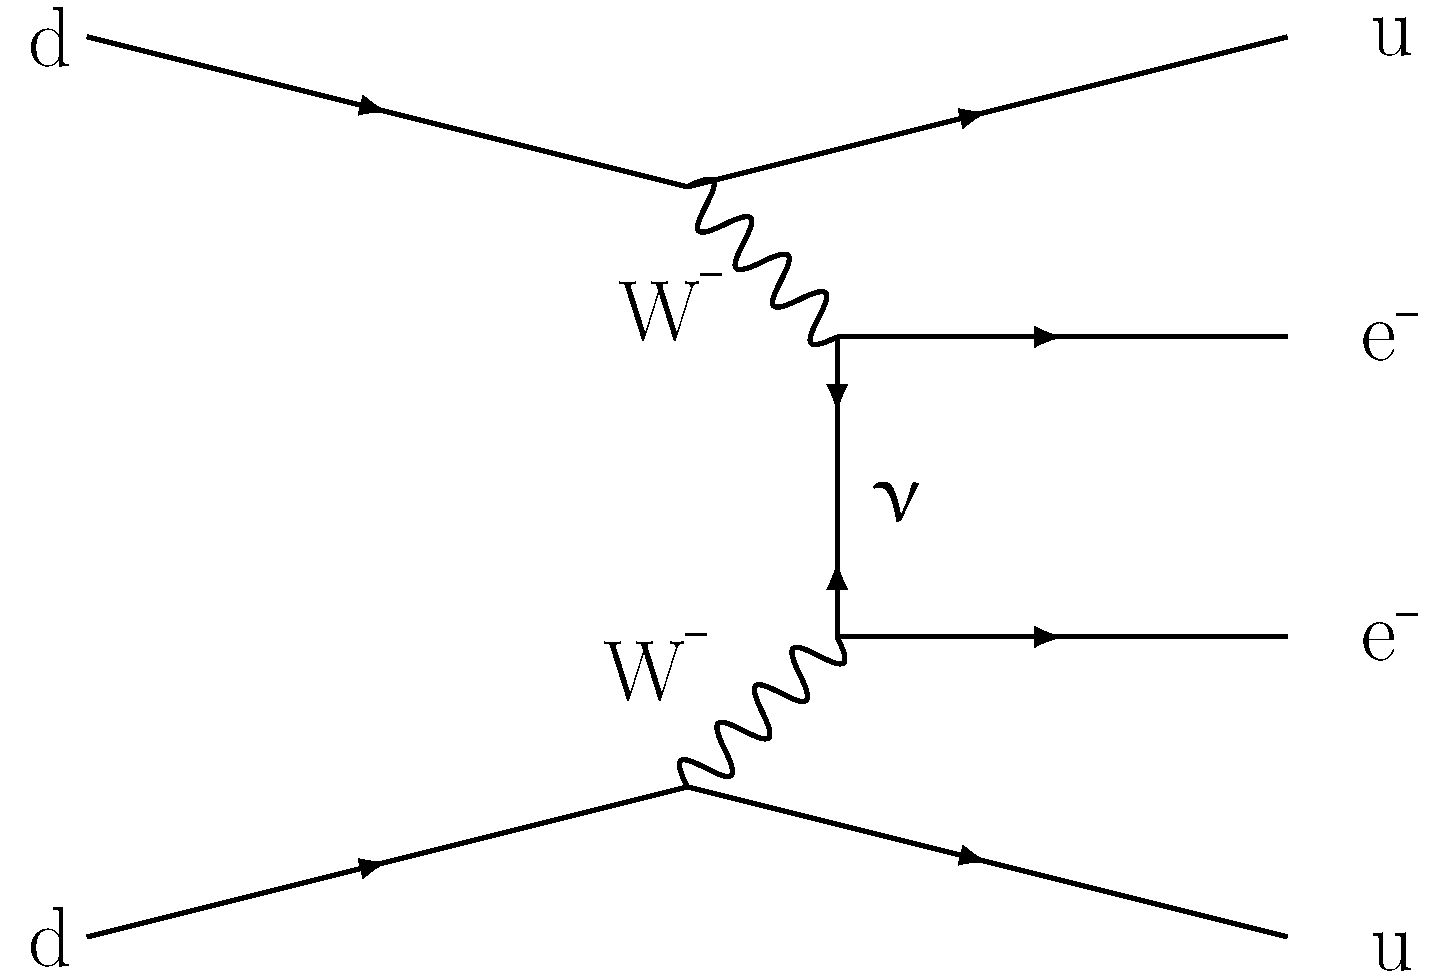
\includegraphics[width=0.4\textwidth]{\currentFigureFolder/double-beta-decay/feynman-double-beta-decay.pdf}
	\xcaption{Feynman graph of neutrinoless double-beta decay}{Feynman graph of neutrinoless double-$\boldsymbol{\upbeta}$ decay.}{The graph depicts the simultaneous transformation of two neutrons into two protons where the down quarks transform into up quarks, whilst two electrons and two neutrinos are produced. The two emitted neutrinos annihilate in a Majorana transition.}
	\label{fig:neutrinoPhysicsAbsoluteNuMassMeasurementDoubleBeta}
\end{figure}

\subsection{Kinematic Measurements of Weak Decays}
\label{sec:neutrinoPhysicsAbsoluteNuMassMeasurementKinematics}
Several laboratory experiments as well as the
supernova event 1987A have provided upper limits of absolute neutrino masses from the analysis of kinematics of weak interactions involving neutrinos or neutrino time-of-flight considerations. Such experiments can not resolve the mass splitting between the squared mass eigenvalues. Therefore, the corresponding observable is an effective mass, respectively a weighted sum of the $N$ neutrino eigenmasses, where the weights are the elements of the PMNS matrix~(eq.~\ref{eq:PMNSmatrix})~\cite{Otten:2008zz}
\begin{equation}
\label{eq:nuMassSquared}
    m^2_{\upnu_{\alpha}} = \sum_{i}^{N}\abs{U_{\alpha i}}^2 m_i^2 \fullstop
\end{equation}
In the scope of this thesis, the measurement of the mass of the electron antineutrino via $\upbeta^-$-decay kinematics is of special interest. Hence, this subject is examined more closely within this section. For completeness, aside from the upper limit on the effective mass of the electron antineutrino, table~\ref{tab:neutrinoPhysicsAbsoluteNuMassMeasurementKinLimits} also lists upper limits for other neutrino flavors obtained by kinematic measurements.
\begin{table}
	\centering
	\xcaption{Constraints on the neutrino mass by kinematic measurements}{Constraints on the neutrino mass by kinematic measurements.}{The table lists upper limits on the absolute neutrino masses for different neutrino flavors.}
	\label{tab:neutrinoPhysicsAbsoluteNuMassMeasurementKinLimits}
		\begin{tabular}{llrr}
		\toprule
		flavor & measurement basis & upper limit & reference \\
		\hline
		$\upnu_\mathrm{e}$ &
		neutrinos from Supernova 1987A &
		\makecell[r]{\SI{5.7}{eV} (\SI{95}{\percent} C.I.)} &
		\cite{Loredo2002} \\
		$\upnu_\upmu$ &
		muon decay &
		\SI{17}{keV} (\SI{90}{\percent} C.L.) &
		\cite{Assamagan1996} \\
		$\upnu_\uptau$ &
		tau decay &
		\SI{18.2}{MeV} (\SI{95}{\percent} C.L.) &
		\cite{Barate:1997zg} \\
		$\aeneutrino$ &
		tritium-$\upbeta$ decay &
		\SI{2}{eV} (\SI{95}{\percent} C.L.) &
		\makecell[r]{\cite{Kraus2005}, \cite{Aseev:2011dq}, \\ \cite{ReviewOfParticlePhysics}} \\
		\bottomrule
	\end{tabular}
\end{table}


\paragraph{Neutrino Masses from $\boldsymbol{\upbeta}$-decay Kinematics} 
In $\upbeta^-$ decay
\begin{equation}
    \ce{X}(Z,A) \rightarrow \ce{Y}(Z+1,A) + \ce{e^-} + \aeneutrino
\end{equation}
part of the released surplus energy generates the neutrino's mass. This leaves a signature in the $\upbeta$ spectrum (see section~\ref{sec:intSpecModelDiffSpec} for a quantitative description). In a neutrino mass experiment four criteria are important for a suitable $\upbeta$ emitter~\cite{Otten:2008zz}:
\begin{itemize}
	\item The $\upbeta$ emitter should have an energy spectrum with a relatively low endpoint because in the uncertainty on the neutrino mass enter the input uncertainties of the neutrino energy and	momentum scaled up with the endpoint energy.
	\item The $\upbeta$ emitter must have a sufficiently high activity to provide statistically relevant count rates for quantities of the $\upbeta$ emitter that can be handled in the laboratory.
	\item The $\upbeta$ decay should be super-allowed in order for the nuclear matrix element of the decay process to be energy independent.
	\item The $\upbeta$-emitter molecule should be as simple as possible to allow for a theoretical treatment of its decay kinematics such as the energy state of the daughter molecule after the decay.
\end{itemize}
Tritium is an ideal candidate with respect to these criteria~\cite{Otten:2008zz}. The corresponding measurement principle will be explained more closely in the following chapters about the KATRIN experiment. However, KATRIN has several predecessor experiments. The most recent two experiments based on tritium-$\upbeta$ decay in Mainz and Troitsk obtained a combined upper limit on the electron antineutrino mass of~\cite{Kraus2005, Aseev:2011dq, ReviewOfParticlePhysics}
\begin{equation*}
    m_{\aeneutrino} < \SI{2}{eV} \quad (\SI{95}{\percent} \text{ C.L.}) \fullstop 
\end{equation*}
It should be noted, that KATRIN aims for a sensitivity that is better by one order of magnitude.
\FloatBarrier
    \def\currentRootFolder{chapter/katrinExperiment}
\def\currentFigureFolder{\currentRootFolder/fig}
\newcommand{\elecIndex}{\mathrm{e}}

\newcommand{\Bsource}{B^j_\mathrm{S}}
\newcommand{\BsourceAvg}{B_\mathrm{S}}
\newcommand{\zSource}{z_\mathrm{S}}
\newcommand{\thetaSource}{\theta_\mathrm{S}}
\newcommand{\thetaSourceAvg}{\theta_\mathrm{S}}
\newcommand{\Esource}{E_\mathrm{S}}
\newcommand{\Usource}{U^j_\mathrm{S}}
\newcommand{\gammaSource}{\gamma_\mathrm{S}}


\newcommand{\Bps}{B_\mathrm{PS2}}
\newcommand{\Bana}{B_\mathrm{A}}
\newcommand{\Bpinch}{B_\mathrm{P}}
\newcommand{\Bmax}{B_\mathrm{max}}
\newcommand{\Bmin}{B_\mathrm{min}}

\newcommand{\thetaMax}{\theta_\mathrm{max}}
\newcommand{\Esur}{E_\mathrm{sur}}
\newcommand{\detEff}{\epsilon_\mathrm{det}}
\newcommand{\macefilterwidth}{\Delta \mathcal{E}^j(\thetaS^j)}

\newcommand{\EtransPure}{E^j_\mathrm{tr}}
\newcommand{\Etrans}{\EtransPure(qU,\Esource,\thetaSource)}
\newcommand{\thetaTransPure}{\theta^j_\mathrm{tr}}
\newcommand{\thetaTrans}{\thetaTransPure(\Esource,qU)}

\newcommand{\As}{A_\mathrm{S}}
\newcommand{\Rbg}{R_\mathrm{bg}}


\newacronym{sts}{STS}{source and transport section}
\newacronym{sds}{SDS}{spectrometer and detector section}
\newacronym{wgts}{WGTS}{windowless gaseous tritium source}
\newacronym{rs}{RS}{rear section}
\newacronym{dps}{DPS}{differential pumping section}
\newacronym{cps}{CPS}{cryogenic pumping section}
\newacronym{tlk}{TLK}{Tritium Laboratory Karlsruhe}
\newacronym{lara}{LARA}{laser Raman system}
\newacronym{bixs}{BIXS}{beta-induced X-ray spectroscopy}
\newacronym{fbm}{FBM}{forward beam monitor}
\newacronym{ckrs}{CKrS}{condensed \ce{^{83m}Kr} source}
\newacronym{mace}{MAC-E}{magnetic adiabatic collimation with electrostatic filtering}
\newacronym{emcs}{EMCS}{Earth magnetic field compensation system}
\newacronym{lfcs}{LFCS}{low-field correction system}
\newacronym{vmms}{VMMS}{vertical magnetic measuring system}
\newacronym{rmms}{RMMS}{radial magnetic measuring system}
\newacronym{fpd}{FPD}{focal plane detector}
\newacronym{pulcinella}{PULCINELLA}{precision ultra-low current integrating normalization electrometer for low-level analysis}
\chapter{The KATRIN Experiment}
\label{sec:katrinExpSetup}
The KArlsruhe TRItium Neutrino (KATRIN) experiment performs a kinematic measurement of the tritium-$\upbeta$~spectrum in order to determine the effective mass of the electron antineutrino (from here forth labeled~$m_\upnu$ and called neutrino mass) as defined by equation~\eqref{eq:nuMassSquared}. In case no neutrino mass signal is observed, KATRIN aims to set an upper limit of
\begin{equation*}
m_\upnu < \SI{200}{meV} \quad (\SI{90}{\percent} \text{ C.L.})
\comma
\end{equation*}
which is one order of magnitude more constraining than the one set by its predecessor experiments.
KATRIN recorded the first $\upbeta$~spectrum in a commissioning run in May 2018 and started neutrino mass measurements in March 2019.

This chapter provides an overview of the KATRIN apparatus. However, given KATRIN's complexity, it can by no means be exhaustive and for a comprehensive treatment the reader is referred to the KATRIN Design Report~\cite{Angrik:2005ep} supplemented by an up-to-date hardware overview that is in the making at the time of writing this thesis\footnote{K. Altenmüller et al. (KATRIN collaboration), in prep.}.
\section{Overview}
\label{sec:katrinExpSetupOverview}
\begin{figure}[t]
	\inputpdftex{\currentFigureFolder/beamline}
	\xcaption{KATRIN beamline}{The KATRIN beamline.}{Shown are the main hardware components:\\
		a) rear section (see section \ref{sec:katrinExpSetupRearSection})\\
		b) \glsentryfull{wgts} (see section \ref{sec:katrinExpSetupWGTS})\\
		c) \glsentryfull{dps} (see section \ref{sec:katrinExpSetupDiffPumpingSection})\\
		d) \glsentryfull{cps} (see section \ref{sec:katrinExpSetupCryoPumpingSection})\\
		e) pre spectrometer (see section \ref{sec:katrinExpSetupSpectrometer})\\
		f) main spectrometer (see section \ref{sec:katrinExpSetupSpectrometer})\\
		g) detector (see section \ref{sec:katrinExpSetupDetector})
	}
	\label{fig:katrinExpSetupBeamline}
\end{figure}
The KATRIN experiment comprises a 70-m-long beam line depicted in figure \ref{fig:katrinExpSetupBeamline}. It can be divided into two sections: 
\begin{enumerate}
	\item Within the \textbf{\gls{sts}} the tritium decays and the $\upbeta$ electrons are magnetically guided along the beam line. Furthermore, the gas flow from the tritium source to the exit of the \gls{sts} is reduced by 14 orders of magnitude.
	\item In the \textbf{\gls{sds}} the $\upbeta$ electrons are filtered according to their kinetic energy and finally counted at the detector.
\end{enumerate}
The $\upbeta$ electrons must be guided from their point of origin to the detector. Therefore, a magnetic filed is created by superconducting coils surrounding the beam line in the \gls{sts} as well as coils around the spectrometer tank in the \gls{sds}. The field lines are parallel to the beam line and intersperse it over the range of the whole experiment. The volume that is mapped onto the detector by this mechanism is called the flux tube. Within the flux tube, charged particles perform cyclotron motions around the field lines and are adiabatically guided from the \gls{sts} to the detector. Adiabaticity is guaranteed by avoiding strongly varying field strengths on short distances. 

As $\upbeta$ electrons must not loose energy before their detection, the \gls{sds} is windowlessly connected to the \gls{sts}. However, the spectrometer must be kept practically free of any tritium flow for safety reasons and to keep the strict background requirements. Therefore, pumping systems reduce the gas inlet pressure of $\sim\SI{3e-3}{mbar}$ to the tritium partial pressure of $\sim\SI{1e-11}{mbar}$ of the spectrometer.

The following sections step through the various components along the KATRIN beam line describing their functionality and purpose.

\section{Windowless Gaseous Tritium Source}
\label{sec:katrinExpSetupWGTS}
\begin{figure}
    \centering    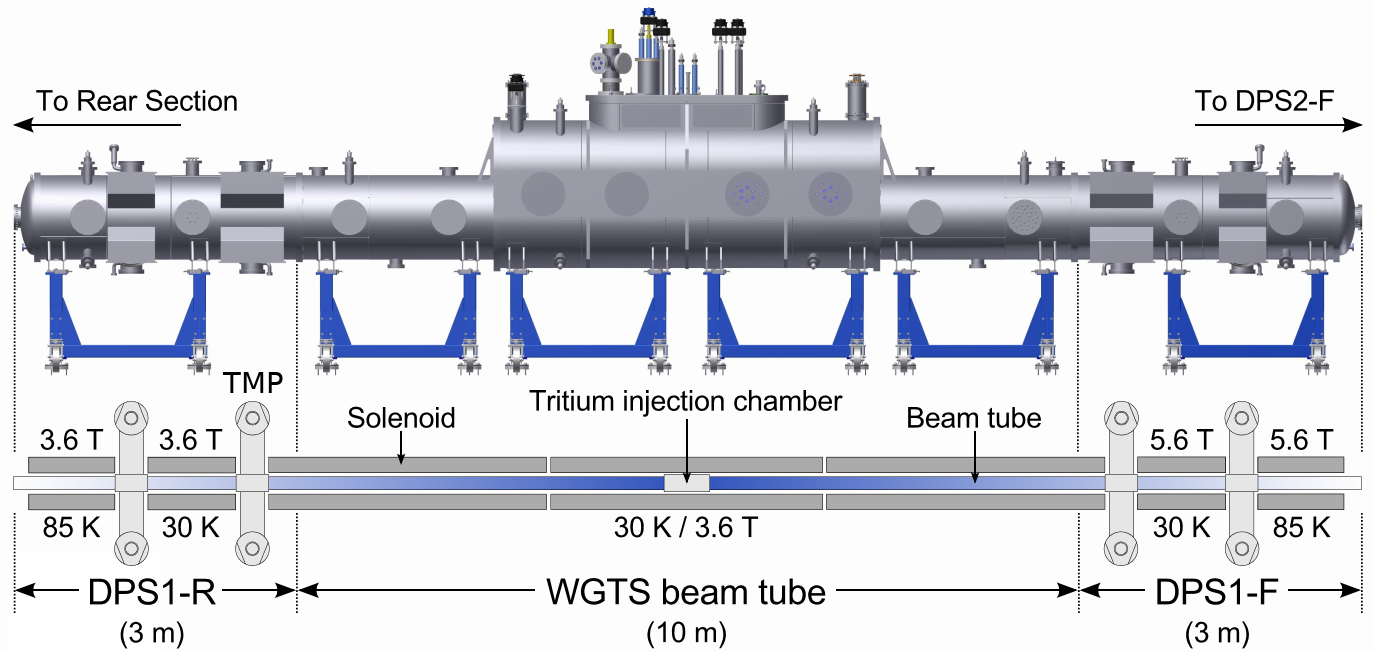
\includegraphics[width=\textwidth]{\currentFigureFolder/wgtsWithTMPLabel.png}
    \xcaption{KATRIN \glsentryfull{wgts}}{The \glsentryfull{wgts}.}{The hull and a sketch of the beam tube are shown. Indicated are the 8 turbo molecular pumps (TMP), the 7 magnets, the design temperatures for tritium operation, the maximum magnetic field strengths and a gradient within the beam tube depicting the decreasing gas density from the center to the sides. (Adapted from \cite{Harms2015}.)}
    \label{fig:katrinExpSetupWGTS}
\end{figure}%
The \gls{wgts} is a 16-m-long, 1.5-m-wide and 4-m-high cryostat. It is depicted in figure \ref{fig:katrinExpSetupWGTS} and a detailed description can e.\,g.~be found in \cite{Grohman2008}. In the following the major features of the \gls{wgts} are reviewed:

{\par\textbf{Tritium purity:} 
The molecular tritium (\ce{T2}) is injected in the middle of the 10-m beam tube of \SI{90}{mm} diameter, where it decays. The design gas column density is 
\begin{equation}
    \label{eq:columnDensity}
    \rho d = \SI{5e17}{molecules/{cm}^2}
\end{equation}
with an isotropic tritium purity of
\begin{equation}
    \epsilon_\text{T} = \SI{95}{\percent}
    \fullstop
\end{equation}
At the front and rear of the \gls{wgts}, the gas is extracted from the beam tube by turbo molecular pumps in designated differential pumping sections called DPS-1-R (rear) and DPS-1-F (front). The extracted gas is re-injected in the center of the beam tube. The respective pipe system is called the inner loop~\cite{PRIESTER201542}. The tritium purity $\epsilon_\text{T}$ must be kept stable on a \SI{0.1}{\percent} level~\cite{Angrik:2005ep}. Therefore, a permeator is installed that separates impurities (like e.\,g.~helium) and ejects them into the exhaust loop of the \gls{tlk}. Furthermore, the isotopic composition of the gas
is monitored by a designated \gls{lara}~\cite{Schloesser2013}.}

{\par\textbf{Injection pressure:}
The design injection pressure of the tritium gas is $1.8\text{\,mbar}\mathcal{l}/\text{s}$. It must be kept stable at the $\SI{0.1}{\percent}$ level. This is achieved via a pressure- and temperature-controlled buffer vessel within the inner loop~\cite{PRIESTER201542}.}

{\par\textbf{Magnetic field:}
In order to adiabatically guide the $\upbeta$ electrons to the spectrometer section the \gls{wgts} is submerged in a magnetic field parallel to its beam tube of up to \SI{5.6}{T}. It is created by 7 superconducting coils, that surround the beam tube. These magnets are kept at a temperature of \SI{4.2}{K} by liquid helium~\cite{Arenz2018}.}

{\par\textbf{Temperature:}
On the one hand, thermal motion smears the energy spectrum of the $\upbeta$ electrons (Doppler effect). On the other hand, at low temperatures the gas molecules cluster. $T=\SI{30}{K}$ is chosen as a compromise and established by a two-phase neon cooling system. For calibration purposes, it is also possible to operate the \gls{wgts} with krypton-83m instead of tritium. This requires a beam tube temperature of $T=100K$ in order for the krypton not to freeze. In this operational mode the neon has to be exchanged for argon~\cite{Angrik:2005ep}.}

\section{Rear Section}
\label{sec:katrinExpSetupRearSection}
\begin{figure}[t]
    \inputpdftex{\currentFigureFolder/rear-section}
   	\xcaption{KATRIN rear section}{The rear section}{terminates the KATRIN beam line and houses several monitoring and calibration devices that are described in the main text. (Adapted from \cite{SeitzM2019}.)}
 \label{fig:rearSection}
\end{figure}

The rear section terminates the beam line in the upstream direction and houses monitoring, calibration and control devices. It is depicted in figure \ref{fig:rearSection} and a detailed description can e.\,g.~be found in \cite{Babutzka2014}. In the following the major features of the rear section are reviewed:

{\par\textbf{Electron gun:}
The rear section houses an electron gun in order to measure the response function of the experiment (see section \ref{sec:response}) via a electron source with a well-defined energy resolution of $\sim \SI{0.2}{eV}$ and angular resolution of $\sim \SI{4}{\degree}$. The electrons are guided towards and through the rear wall by a designated electromagnetic guidance system. Furthermore, their flight path can be adjusted by dipole magnets mounted in the \gls{wgts} which enables a scanning of the full flux tube~\cite{Babutzka2014}.}

{\par \textbf{Rear wall and plasma control:}
The so-called rear wall is a gold-coated stainless-steel disc with a diameter of 6 inches that terminates the beam tube. It has a hole in the center to let electrons from the electron gun pass through. Its main purpose is the control of plasma effects: Space charges, respectively a plasma, forms within the \gls{wgts} due to the tritium decay. Therefore, $\upbeta$ electrons may start at different potentials which adds uncertainty to the measured $\upbeta$ spectrum. Simulations show that the plasma can be influenced by the rear wall potential which can be controlled via a voltage supply in the range of $\pm \SI{10}{V}$. Moreover, a UV light illumination of the rear wall can extract electrons via the photoelectric effect that can compensate space charges. Therefore, a homogeneous work function of the rear wall with fluctuations less than \SI{20}{meV} is required~\cite{Kuckert2018, Kuckert2016}.}

{\par\textbf{Activity monitoring:}
A super conducting coil designed to create a magnetic field of \SI{4.7}{T} in the rear section ensures that the magnetic flux tube terminates at the rear wall. Hence, per design of the magnetic guidance, $\upbeta$ electrons either arrive at the detector or hit the rear wall. On hitting the rear wall they emit bremsstrahlung. Two dedicated \gls{bixs} systems measure the corresponding X-ray spectrum to determine the source strength respectively the gas column density, equation~\eqref{eq:columnDensity}~\cite{Roellig2015}.}

\section{Differential Pumping Section}
\label{sec:katrinExpSetupDiffPumpingSection}
\begin{figure}[t]
    \inputpdftex{\currentFigureFolder/dps}
   	\xcaption{KATRIN \glsentryfull{dps}}{The \glsentryfull{dps}}{reduces the gas flow by five orders of magnitude and blocks tritium ions. Its five elements, each with a separate magnet (M1-M5), and connected by pump ports, are shown. The outer loop connects the turbo molecular pumps to the infrastructure of the \gls{tlk}. (Adapted from \cite{SeitzM2019}.)}
 \label{fig:katrinExpSetupDiffPumpingSection}
\end{figure}
The \glsentryfull{dps} is composed of five elements. It is depicted in figure \ref{fig:katrinExpSetupDiffPumpingSection} and a detailed description can e.\,g.~be found in~\cite{Kosmider2012}. For orientation, in this section, the elements are labeled 1 to 5 from \gls{wgts} to \gls{cps}. The major features of the \gls{dps} are reviewed in the following:

{\par\textbf{Reduction of tritium flow:}
The five beam tube elements of the \glsentryfull{dps} form a \SI{20}{\degree} angle to each other and are arranged in a chicane. $\upbeta$~electrons are magnetically guided along the chicane by a magnetic field of up to \SI{5.5}{T} created by five superconducting solenoids. By contrast, the neutral gas molecules scatter off the walls. This reduces the molecular beaming effect and enhances the pumping probability~\cite{ZHANG2012}. Four turbo molecular pumps mounted between the beam tube elements then reduce the gas flow by approximately five orders of magnitude and feed the gas into the so-called outer loop where it is reprocessed~\cite{Kosmider2012}.}

{\par\textbf{Ion blocking:}
In the \gls{wgts}, ions such as \ce{HeT^+}, \ce{T_2+}, \ce{T_3+}, \ce{T_5+} can form. If they were not blocked, they would reach the spectrometer section together with the $\upbeta$~electrons and would be even accelerated by the retarding voltage (see section~\ref{sec:katrinExpSetupSpectrometer}). This would eventually lead to an increased background rate. A potential barrier created by two ring electrodes in element 5 and the pump port between \gls{dps} and \gls{cps} set to $+\SI{100}{V}$ avoids such a scenario. The positive ions are deflected, and dipole electrodes in the elements 1 to 4 make them drift out of the flux tube. They hit the wall and get neutralized~\cite{Klein2019}.}

{\par\textbf{Ion monitoring:}
Downstream of the blocking electrodes, the remaining ion flux is measured by a Fourier transform ion cyclotron resonance device (FT-ICR)~\cite{Ubieto2009}.}

\section{Cryogenic Pumping Section}
\label{sec:katrinExpSetupCryoPumpingSection}
\begin{figure}[t]
    \inputpdftex{\currentFigureFolder/cps}
   	\xcaption{KATRIN \glsentryfull{cps}}{The \glsentryfull{cps}}{is the coldest part of the KATRIN experiment. It consists of seven elements, labeled by 1 to 7 from the \gls{dps} to the pre spectrometer. Elements 2 to 5 are covered by a frozen argon layer at~\SI{3}{K} in order to cold-trap tritium molecules. The low temperatures are established using liquid helium (\ce{LHe}) and an insulation of liquid nitrogen (\ce{LN2}). Each element is enclosed by a super conducting coil (M1 to M7) for magnetic guidance of the $\upbeta$~electrons. For the \glsentryshort{fbm} and the \glsentryshort{ckrs} the reader is referred to the main text. (Adapted from \cite{SeitzM2019}.)}
 \label{fig:katrinExpSetupCryoPumpingSection}
\end{figure}
The \glsentryfull{cps} is an approximately 7-m-long cryostat. It is depicted in figure \ref{fig:katrinExpSetupCryoPumpingSection} and a detailed description can e.\,g.~be found in \cite{Jansen2015}. For orientation, in this section, its seven elements are labeled by 1 to 7 from \gls{wgts} to \gls{cps}. The major features of the \gls{cps} are reviewed in the following:

{\par\textbf{Reduction of tritium flow:}
The \gls{cps} consists of seven beam tube elements, of which the first five are arranged in a chicane forming~\SI{15}{\degree} angles, in a similar manner as the beam tube elements of the \gls{dps}. Charged particles are guided along the chicane by a magnetic field of up to~\SI{5.6}{T} created by seven superconducting coils. Neutral molecules hit the walls, that are covered by a frozen argon layer cooled down to~\SI{3}{K} in order to cold-trap particles. These low temperatures are achieved via liquid helium cooling and a heat shield of liquid neon. After the accumulation of about~\SI{1}{Ci} of tritium, the argon frost layer has to be renewed. In order to achieve this, the beam tube is warmed up and the argon is pumped off along with the accumulated tritium. Tests and simulations show a reduction of the tritium flow by approximately 10 orders of magnitude from the entrance to the exit of the \gls{cps}~\cite{Jansen2015,Roettele2019}.}

{\par\textbf{The \glsentryfull{fbm}}: 
The \glsentryshort{fbm} can be moved horizontally into the pump port between beam tube element 6 and 7 of the \gls{cps} with a 2-dimensional spatial resolution of \SI{0.1}{mm}. Two \textit{pin}-diodes measure the $\upbeta$-electron flux and thus the stability of the gas column density in the \gls{wgts}. Furthermore, the \gls{fbm} equips a temperature and a hall sensor. A second detector board holding a Faraday cup for ion measurements is also available~\cite{Klein2019}. More information about the \gls{fbm} can e.\,g.~be found in \cite{Ellinger2017,Ellinger2019}.}

{\par\textbf{The \glsentryfull{ckrs}:} The \gls{ckrs} is a sub mono-layer of \kryptonEightyThree{} on a pyrolytic graphite substrate with a diameter of \SI{2}{cm}. It can be lowered in the pump port of the \gls{cps} and moved in a 2-dimensional plane perpendicular to the beam line. This enables the spatial scanning of the properties of the spectrometer using quasi-monoenergetic conversion electron lines of \kryptonEightyThree~\cite{Bauer2014, Dyba2019, Arenz2018Kr}.}

\section{Pre and Main Spectrometer}
\label{sec:katrinExpSetupSpectrometer}
The pre and main spectrometer are vacuum vessels designed to filter passing electrons according to their kinetic energy. The pre spectrometer has a length of \SI{3.4}{m} and a diameter of \SI{1.7}{m}. Details on its design can e.\,g.~be found in \cite{Valerius2009,Fraenkle2010}. The main spectrometer has a length of \SI{23}{m} and a diameter of \SI{10}{m}. Details on its design can e.\,g.~be found in \cite{Valerius2009, Valerius2004}. The functionality and purpose of spectrometer related aspects are reviewed in this section. The content is divided into two parts: Section \ref{sec:katrinExpSetupSpectrometerMACE} explains the so-called MAC-E filter principle and section \ref{sec:katrinExpSetupSpectrometerBGCounterMeasures} list several measures to keep the strict KATRIN background requirements.

\subsection{MAC-E-Filter Principle}
\label{sec:katrinExpSetupSpectrometerMACE}
\begin{figure}[t]
	\inputpdftex{\currentFigureFolder/mace}
	\xcaption{Scheme of the KATRIN main spectrometer and the \glsentryshort{mace} filter principle.}{
		Scheme of the KATRIN main spectrometer and the \glsentryfull{mace} filter principle.}{
		The {KATRIN} design magnetic field settings are
		$\Bps=\SI{4.5}{T}$, 
		$\Bsource=\SI{3.6}{T}$, 
		$\Bmax=\SI{6.0}{T}$, 
		$B_\mathrm{D}=\SI{3.6}{T}$, 
		$\Bana\approx\SI{3e-4}{T}$. $\Vec{E}$ denotes the magnetic field regulated by the retarding potential $U$ that reaches its maximum $U_\mathrm{a} = U$ at the analyzing plane. (Adapted from \cite{SeitzM2019}.)
	}
	\label{fig:katrinExpSetupSpectrometer}
\end{figure}
The pre and main spectrometer are based on the principle of the so-called \gls{mace}~\cite{Beamson1980}. It enables the filtering of electrons according to their kinetic energy. Figure~\ref{fig:katrinExpSetupSpectrometer} sketches the \gls{mace} filter of KATRIN. The following paragraphs outline the basic concepts and their experimental implementation. As the principle is of key importance for the KATRIN experiment, it is additionally treated in a mathematical way in the subsequent section~\ref{sec:intSpecModelResponseTransmission}.

{\par \textbf{Electrostatic filtering:}
A retarding voltage barrier is applied along the beam axis within the spectrometer, reaching its maximum $U$ at the so-called analyzing plane in the center and dropping off towards the source section and the detector. The retarding voltage barrier deflects electrons with kinetic energies below $eU$. For higher energies, whether an electron can pass the spectrometer or not depends on the angle between its direction of motion and the magnetic field lines (see eq.~\ref{eq:intSpecModelTransmission} for a quantitative description). 

{\par \textbf{Magnetic collimation}: 
The electric field gradient of the retarding voltage barrier is parallel to the beam line, but $\upbeta$~electrons are emitted in an arbitrary angle with respect to the magnetic field lines. In order to analyze their full kinetic energy, they have to be collimated. This is achieved by a magnetic field gradient that drops from $\Bsource=\SI{3.6}{T}$ in the \gls{sts} to $\Bana\approx\SI{3e-4}{T}$ in the analyzing plane. In the following, a plausibility argument for the momentum collimation due to the field gradient, according to~\cite{Angrik:2005ep}, is given: Electrons entering the spectrometer vessel perform cyclotron motions around the magnetic field lines. Their total kinetic energy~$\Esource$ is split into a longitudinal component~$E_\parallel$ along the beam axis and a transverse component~$E_\bot$
\begin{equation}
\label{eq:totalKinElecEnergy}
\Esource = E_\parallel + E_\bot \fullstop
\end{equation}
In the non-relativistic and adiabatic approximation, the transverse component can be expressed by the magnetic field strength~$B$ and the electron's magnetic moment~$\mu$ respectively its charge~$q=e$, its mass~$m_\elecIndex$ and angular momentum~$L$~\cite{jackson1975classical}
\begin{equation}
E_\bot = - \mu B = \frac{e}{2 m_\elecIndex}LB \fullstop
\end{equation}
Adiabaticity conserves the angular momentum $L$ and the total energy of the electron $\Esource$ along its trajectory. Hence, when the magnetic field strength $B$ decreases to $\Bana=\Bmin$ in the analyzing plane, the transverse component of the electron's energy $E_\bot$ decreases likewise and transforms to longitudinal energy $E_\parallel$.}

{\par \textbf{Magnetic Bottle effect:}
As the source is placed in a lower magnetic field $\Bsource$ compared to the maximum field strength along the beam line $\Bmax$ at the detector side, $\upbeta$~electrons traveling downstream to the detector are subject to the magnetic bottle effect~\cite{Angrik:2005ep}. They get reflected and travel upstream to the rear wall if their starting angle $\thetaSource$ with respect to the beam line axis surpasses $\thetaMax$ with
\begin{equation}
\label{eq:thetaMax}
\sin\thetaMax = \sqrt{\frac{\Bsource}{\Bmax}} 
\fullstop
\end{equation}
For the KATRIN design values $\Bmax=\SI{6}{T}$ and $\Bsource=\SI{3.6}{T}$ one obtains $\thetaMax\approx\SI{51}{\degree}$.
A cutting angle $\thetaMax$ is beneficial because the greater the emission angle of a $\upbeta$~electron the larger the distance it travels in the \gls{wgts} and the more it is subject to energy losses such as scattering or synchrotron radiation~\cite{Angrik:2005ep}.}

{\par \textbf{\gls{mace}-filter width:} 
Electrons with a kinetic energy below $qU$ cannot pass the spectrometer. Electrons with a kinetic energy above $qU+\Delta E$ do pass the spectrometer. Here, $\Delta E$ denotes the filter width \cite{Angrik:2005ep}
\begin{equation}
\label{eq:katrinExpSetupFilterWidth}
\Delta E = \frac{\Bana}{\Bmax} E
\fullstop
\end{equation}
Electrons with an energy between $eU$ and $eU+\Delta E$ pass the potential barrier only with a certain probability. A quantitative description of this so-called transmission probability is given in the subsequent section~\ref{sec:intSpecModelResponseTransmission}. However, it can already be deduced, that a larger $\Delta E$ adds a greater uncertainty to the measurement and thus it should be kept as low as possible. $\Delta E$ depends on the maximum magnetic field strength along the beam line $\Bmax=\SI{6}{T}$, the kinetic energy of $\upbeta$~electrons $E\approx\SI{18.6}{keV}$, and the magnetic field in the analyzing plane $\Bana\approx\SI{3e-4}{T}$. Hence, its KATRIN design value is $\Delta E\approx\SI{0.93}{eV}$. }

{\par \textbf{Dimensions of the KATRIN main spectrometer:} This paragraph outlines, why the diameter of the KATRIN main spectrometer is \SI{10}{m}, while the one of its predecessor experiment in Mainz was only \SI{1}{m}~\cite{Kraus2005}. KATRIN's envisaged sensitivity requires a relative \gls{mace}-filter width of at least $\Delta E/E = 1/20000$, which directly corresponds the ratio of the magnetic fields $\Bmax/\Bana$~(see eq.~\ref{eq:katrinExpSetupFilterWidth}). For a smaller $\Delta E$, $\Bana$ should be chosen as low as possible. However, the lower $\Bana$, the wider the flux tube that must be governed by the spectrometer vessel. Also, the magnetic field must decrease at a sufficiently slow rate from the spectrometer's entrance to the analyzing plane in order to guarantee adiabaticity, which requires a certain spectrometer length. Dimensions that meet the demands and are feasible for the main spectrometer were found to be a radius of \SI{10}{m} and a length of \SI{23}{m}~\cite{Angrik:2005ep, Valerius2004}.}

Given the requirements on the magnetic and electrostatic fields, the following two paragraphs review their technical implementation:

{\par \textbf{Magnetic field:} The main spectrometer is surrounded by a system of coils that shapes the \gls{mace} filter's  magnetic field. Upstream, there is the PS2 magnet ($\Bmax=\SI{4.5}{T}$); downstream the pinch ($\Bpinch=\Bmax=\SI{6.0}{T}$) as well as the detector magnet ($B_\mathrm{D}=\SI{3.6}{T}$), which are superconducting solenoids. The field is fine-tuned by a system of air coils around the spectrometer hull: There is the \gls{emcs} with 26 current loops parallel to the beam line axis. Furthermore, there is the \gls{lfcs} with 14 air coils perpendicular to the beam line axis. The combined system constrains the electrons' flux tube to the spectrometer vessel and compensates the Earth's magnetic field as well as effects from ferromagnetic materials in the spectrometer's surroundings~\cite{Erhard2018}. Additionally, a vertical and radial magnetic measuring system (\glsentryshort{vmms} and \glsentryshort{rmms}) are installed outside the spectrometer vessel. The field inside the spectrometer vessel is assessed via samples of these measuring systems combined with simulations~\cite{Letnev2018}.}

{\par \textbf{Electrostatic field:} A high-voltage system establishes the \gls{mace} filter's retarding potential. The fluctuation of the retarding voltages must have a standard deviation smaller than \SI{60}{mV} for the envisaged sensitivity to the neutrino mass~\cite{Angrik:2005ep}. The antenna-like beam line setup is sensitive to electromagnetic fluctuations of any source, which is why an active post-regulation system for the voltage is deployed. It monitors the retarding potential and regulates it with the required precision. For the monitoring the monitor spectrometer and a voltage divider are deployed. For details on the later systems the reader is referred to~\cite{Thuemmler2009,Erhard2014,Zboril2011}.}

\subsection{Background Mitigation Strategies}
\label{sec:katrinExpSetupSpectrometerBGCounterMeasures}
The KATRIN sensitivity goal requires a background rate of less than \SI{10}{mcps}~\cite{Angrik:2005ep}. Several background-related aspects with respect to the spectrometer tanks are listed below:

{\par \textbf{Vacuum:} The spectrometers are operated at a pressure on the order of \SI{1e-11}{mbar}. This prevents electron scattering on residual gas and minimizes background effects by ionization. Correspondingly, turbo molecular and getter pumps are installed at three pump ports of the spectrometer vessels. Furthermore, the spectrometers can be baked out at up to \SI{350}{\celsius}~\cite{Arenz2016}.}
	
{\par \textbf{Wire electrodes:} The inner walls of the spectrometer vessels are lined by wire electrodes. Their potential is a few hundred volts more negative than the spectrometer hull reflecting electrons coming from the vessel walls. Such electrons may be induced by cosmic rays~\cite{Valerius2009}.}
	
{\par \textbf{Ion blocking:} Analogously to the ones in the \gls{cps} (section \ref{sec:katrinExpSetupCryoPumpingSection}), three blocking electrodes are installed; one between the \gls{cps} and the pre spectrometer, one between the pre and main spectrometer; and one between the main spectrometer and the detector~\cite{Klein2019}.}
	
{\par \textbf{Tandem setup:} $\upbeta$~electrons may scatter on residual gas. This can either directly lead to secondary electrons or create positive ions that travel down the beam line. The positive ions in turn may again yield secondary electrons through scattering. The more $\upbeta$~electrons enter the main spectrometer, the higher is the probability to create secondary electrons. In order to reduce the flux of $\upbeta$~electrons into the main spectrometer, the retarding potential of the pre spectrometer is set to a few hundred volts more positive than the one of the main spectrometer. On the one hand, this is a countermeasure against background events, but, on the other hand, charged particles can be trapped between the two spectrometers due to the electromagnetic setup (Penning trap). A sudden discharge may harm the hardware, especially the detector. Therefore, it is possible to sweep a charged wire through the volume in order to collect the trapped particles and avoid this ``Penning discharges''~\cite{Valerius2009}.}
\section{Detector Section}
\label{sec:katrinExpSetupDetector}
\begin{figure}[t]
    \inputpdftex{\currentFigureFolder/detector-section}
   	\xcaption{KATRIN detector section}{The detector section}{terminates the KATRIN beam line. Among other instruments, it houses the \glsentryfull{fpd} for $\upbeta$~electrons with the detector wafer at its core. For an explanation of the other components the reader is referred to the main text. (Adapted from \cite{SeitzM2019}.)}
 \label{fig:katrinExpSetupDetector}
\end{figure}

The detector section terminates the beam line in downstream direction. It can be separated from the spectrometer section by closing a gate valve. The detector section is depicted in figure \ref{fig:katrinExpSetupDetector} and a detailed description can e.g. be found in \cite{Amsbaugh2015}. The major features of the detector section are reviewed in the following:

{\par \textbf{\Gls{fpd}}: The \gls{fpd} counts the $\upbeta$~electrons that pass the spectrometer section. It is a \textit{pin}-silicon detector with a sensitive area of \SI{9}{cm} diameter. It is subdivided in 148 pixels of the same area arranged in 12 rings of 12 pixels each and the so-called bull's eye of 4 pixels in the center. This arrangement allows later correction for radial electrical, magnetic and gas dynamical inhomogeneities in the beam line~\cite{Amsbaugh2015}.}

{\par \textbf{Shield and veto system:} The radiation shield of the \gls{fpd} system consists of two nested cylindrical shells: an outer lead shell of \SI{3}{cm}, that reduces photon background and an inner copper shell of \SI{1.27}{cm}, that blocks X-rays originating from the outer lead shell. The shield is surrounded by a veto system to tag incoming muons. Such a system is necessary to keep the strict background requirements~\cite{Amsbaugh2015}.}

{\par \textbf{Calibration:} Photoelectron sources can be lowered in the line of sight of the detector. The corresponding photocurrent can be measured with the \gls{pulcinella} system. A comparison of \gls{pulcinella} and the \gls{fpd} yields the \gls{fpd}'s detection efficiency. It was determined to be $\epsilon_\mathrm{det}=95\pm1.8\pm2.2\,\text{\%}$~\cite{Amsbaugh2015}.}

{\par \textbf{Detector magnet:} The detector magnet ($B_\mathrm{D}=\SI{3.6}{T}$) allows to form the flux tube near the detector independently of the main spectrometer magnetic field setting. It especially allows its mapping on the the detector~\cite{Amsbaugh2015}.}

{\par \textbf{Post-acceleration electrode:} The post-acceleration potential shifts the electrons arriving from the main spectrometer to a more favorable energy region. This increases the detector efficiency and, additionally, $\upbeta$~electrons can be distinguished from noise originating in the detector by an energy region of interest cut. An appropriate setting was found to be~$\sim\SI{10}{keV}$~\cite{Amsbaugh2015}.}

    \def\currentRootFolder{chapter/modelOfIntegratedRate}
\def\currentFigureFolder{\currentRootFolder/fig}
\newacronym{ssc}{SSC}{source and spectrum calculation}

\newcommand{\fermiConst}{G_\mathrm{F}}
\newcommand{\diffRate}{\frac{\d\Gamma(\Esource)}{\d \Esource}}
\newcommand{\nucMatrixElement}{M_\mathrm{nuc}}
\newcommand{\thetaFunc}{\Theta}

\newcommand{\nuMass}{m_\upnu}

\chapter{Mathematical Model of a KATRIN Measurement}
\label{sec:intSpecModel}
For neutrino mass inference from data or simulation a mathematical model of a KATRIN neutrino mass measurement is required. As parameter inference is of importance within the scope of this thesis, a mathematical formalism describing a KATRIN neutrino mass measurement is outlined within this chapter. Therefore, an expression for the $\upbeta$-decay rate of a tritium molecule is given in section~\ref{sec:intSpecModelDiffSpec}. Section~\ref{sec:intSpecModelResponse} describes the KATRIN response function, respectively the mathematical modeling of the KATRIN apparatus. Sections~\ref{sec:intSpecModelIntegralRate} to~\ref{sec:intSpecModelMTD} translate these concepts into a model of electron counts at the KATRIN detector. Finally, section~\ref{sec:intSpecModelNuMassMeasurement} shows a full simulated KATRIN neutrino mass measurement.

\section{Differential Tritium-\texorpdfstring{$\upbeta$}{Beta}-Decay Spectrum}
\label{sec:intSpecModelDiffSpec}
\begin{figure}
	\centering
	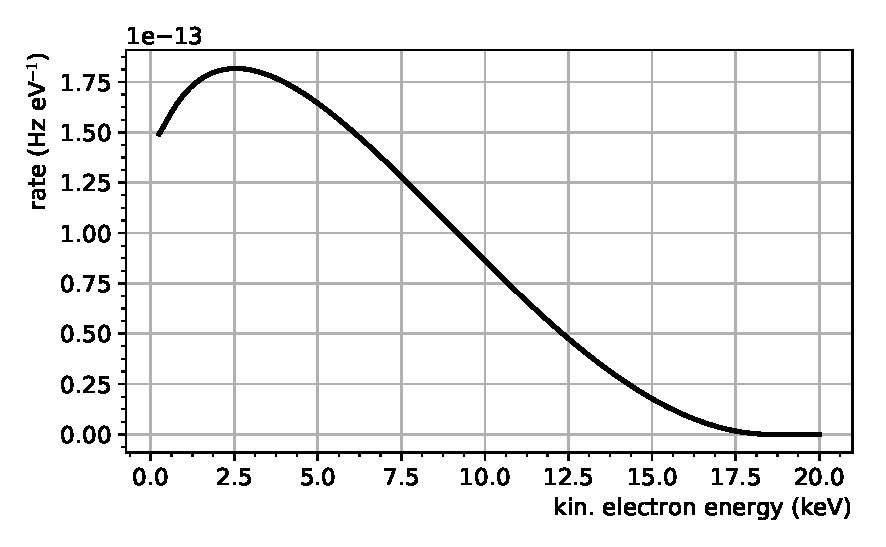
\includegraphics[width=\textwidth]{\currentFigureFolder/diffSpec.pdf}
	\xcaption{Tritium-$\upbeta$ spectrum for a vanishing and non-vanishing neutrino mass}{Tritium-$\upbeta$ spectrum for a vanishing and non-vanishing neutrino mass.}{The plot shows the differential rate as described by equation \eqref{eq:intSpecModelDiffSpec} for a vanishing and non-vanishing neutrino mass. (The spectrum was calculated using the SSC software framework, see section \ref{sec:statMethodsKaFitSSC}, neglecting the sum over the final molecular states.) The inset zooms into the endpoint region where a non-vanishing mass causes a shift and a distortion of the spectrum.}
	\label{fig:intSpecModelDiffSpec}
\end{figure}


This section presents a quantitative expression for the $\upbeta$-decay rate of a tritium molecule in dependence on the kinetic energy of the emitted $\upbeta$ electron (differential rate). The following paragraphs describe the differential rate in a top-down approach. In other words, first the whole mathematical description is denoted, then its components are explained.

Using Fermi theory and Fermi's golden rule the decay rate of a tritium molecule is~\cite{Kleesiek2019,Otten:2008zz} 
\begin{align}
\label{eq:intSpecModelDiffSpec}
\diffRate = &
\frac{\fermiConst^2 \abs{V_\mathrm{ud}}^2}{2 \pi^3}
\abs{\nucMatrixElement}^2 \cdot
F(Z, \Esource) \cdot 
p(\Esource+m_\elecIndex) \cdot 
\sum_{f} 
	P_f \cdot 
	\epsilon_f \cdot 
	\sqrt{\epsilon_f^2-\nuMass^2} \cdot 
	\thetaFunc(\epsilon_f-\nuMass)
	\fullstop
\end{align}
Its constituents are the kinetic electron energy $\Esource$;
the effective electron-antineutrino mass $\nuMass$ defined via the PMNS matrix $U$, equation \eqref{eq:PMNSmatrix},
\begin{equation}
	 \nuMass^2 = \abs{U_{\elecIndex i}}^2 m_i^2\,;
\end{equation}
the Fermi constant $\fermiConst$;
the up-down-quark-coupling given by the Cabibbo angle $\theta_\mathrm{C}$~\cite{ReviewOfParticlePhysics}
\begin{equation}
V_\mathrm{ud} = \cos \theta_\mathrm{C} = 
0.97425\pm0.00022;
\end{equation}
and the nuclear transition matrix element~\cite{ReviewOfParticlePhysics}
\begin{equation}
\abs{\nucMatrixElement}^2 = g_V^2+3g_A^2 \quad
\text{with } g_V = 1 \quad
\text{and} \quad g_A/g_V = -1.2646 \pm 0.0035
\end{equation}
which is independent of the electron's kinetic energy as the decay is super-allowed and given by the vector $g_V$ and axial vector $g_A$ coupling.

Furthermore, the Fermi function $F(Z,\Esource)$ accounts for the Coulomb interaction between the outgoing electron and the daughter nucleus with atomic charge $Z=2$, which in its relativistic version can be approximated as~\cite{Simpson1981}
\begin{equation}
F(Z,\Esource) \approx \frac{2 \pi \eta}{1-\exp{2 \pi \eta}} \cdot R
\comma
\end{equation}
with Sommerfeld parameter $\eta = \alpha Z / \beta$, fine structure constant $\alpha$, relativistic velocity $\beta$ and a relativistic correction factor $R = 1.002037-0.001427\beta$~\cite{Kleesiek2019}.

The phase-space factor of the outgoing electron with momentum $p$ and mass $m_\elecIndex$ is given by the factor $p(\Esource+m_\elecIndex)$.

The phase space factor of the emitted neutrino  depends on multiple quantities: First, there is the $\upbeta$-spectrum endpoint of molecular tritium $E_0=\SI{18574.00\pm0.07}{eV}$~\cite{Myers2015,Otten:2008zz}. Second, there is the final state energy of the molecular system $V_f$. The exited energy state $f$ is caused by vibration, rotation or electronic excitation of the decaying molecule. A review on tritium molecular final states and tabulated values can e.\,g.~be found in~\cite{Bodine2015} and references therein. The probability that the molecular system is in a final state of energy $V_f$ after the decay is denoted by $P_f$. Then the energy of the neutrino reads 
\begin{equation}
\label{eq:intSpecModelDiffSpecNeutrinoEnergy}
\epsilon_f = E_0 - E - V_f 
\fullstop
\end{equation}
Third, there is the neutrino's momentum $\sqrt{\epsilon_f^2-\nuMass^2}$. Then, the complete phase space factor of the neutrino is a sum over all possible molecular final states labeled $f$.

Lastly, the Heavyside step function $\thetaFunc$ ensures a positive kinetic energy of the neutrino.

In summary, a mathematical description of the differential tritium-$\upbeta$-decay spectrum in dependence of the neutrino mass is possible. Accordingly, the differential rate is depicted in figure~\ref{fig:intSpecModelDiffSpec} for a vanishing and non-vanishing effective electron-antineutrino mass. These results form the foundation for neutrino mass inference at KATRIN. The next sections will relate them to the KATRIN apparatus.

\section{Response Function}
\label{sec:intSpecModelResponse}
The aim of this chapter is the derivation of a formula for the electron rate at the KATRIN detector. Section~\ref{sec:intSpecModelDiffSpec} derived the $\upbeta$-electron rate in dependence of the $\upbeta$-electron energy. The next step is the inclusion of the characteristics of the KATRIN experimental setup. This can be accomplished by denoting the so-called KATRIN response function. It reflects the probability of a electron emitted in the \gls{wgts} to reach the KATRIN detector~\cite{Groh2015}.

Within this section the formalism for the KATRIN response function is developed in a bottom-up approach. First, central concepts and the nomenclature are presented in section~\ref{sec:intSpecModelResponseConcepts}. Then, components of the response function are introduced: 
\begin{itemize}
	\item The gas dynamics within the \gls{sts} need to be simulated. See section~\ref{sec:intSpecModelResponseGasDynamics}.
	\item The characteristics of the KATRIN spectrometer can be summarized in the so-called transmission function. See section~\ref{sec:intSpecModelResponseTransmission}.
	\item The passage of electrons through the \gls{wgts} is characterized by scattering from gas molecules. The probability for such scattering is discussed in section~\ref{sec:intSpecModelResponseScattering}. Furthermore, the amount of energy an electron loses when scattering is considered in section~\ref{sec:intSpecModelResponseEloss}.
\end{itemize}
Finally, the described components will be assembled to the KATRIN response function in section~\ref{sec:intSpecModelResponseReconciliation}.
\subsection{Concepts and Nomenclature}
\label{sec:intSpecModelResponseConcepts}
Before the formalism for the KATRIN response function is developed, this section introduces naming conventions and useful concepts. 

\paragraph{Coordinate System}
This chapter focuses on a one-dimensional description of the KATRIN response function. The position along the beam line is denoted with $z$. The origin of the coordinates system is the center of the \gls{wgts} as already chosen in previous works, e.\,g.~\cite{Groh2015,Kleesiek2014}. In this sense, the rear and the front of the \gls{wgts} of length $d$ have the coordinates $\mp d/2$.

\paragraph{Pitch Angle}
Within this chapter the angle between an electron's direction of motion and the beam line axis, the so-called pitch angle, is denoted by $\theta$.

\paragraph{Parameter Indices}
Whether an electron reaches the KATRIN detector depends i.\,a.~ on its parameters when originating in the \gls{wgts}. Within this chapter these starting parameters are denoted with a lower index $\mathrm{S}$. The three decisive starting parameters are the following:
\begin{enumerate}
	\item The starting kinetic energy $\Esource$ as discussed within the description of the differential rate in equation~\eqref{eq:intSpecModelDiffSpec}.	
	\item The starting position $\zSource$ within the \gls{wgts}.
	\item The starting pitch angle $\thetaSource$ within the \gls{wgts}.
\end{enumerate}
Parameters that denote quantities in the analyzing plane (see section~\ref{sec:katrinExpSetupSpectrometer}) are denoted with a lower index $\mathrm{A}$.

\paragraph{Probabilistic Treatment of  the Starting Pitch Angle}
It should be noted, that the three listed starting parameters are not known for a single $\upbeta$ electron, which suggests a probabilistic treatment. Within the scope of this thesis this is of importance with respect to the starting pitch angle. Therefore, the concept is explained in the following:

Given the distribution $\omega(\thetaSource)$ of starting pitch angles, the mean value of any function $g(\thetaSource)$ depending on a fixed starting pitch angle $\thetaSource$ can be calculated within an interval $[0, \thetaMax]$ by applying the definition of the mean value
\begin{equation}
\label{eq:intSpecModelPitchAngleAveraging}
\mean{g(\thetaSource)} = 
\frac{
	\int_{0}^{\thetaMax} 
	\omega(\thetaSource)
	g(\thetaSource)
	\d \thetaSource   
}{
	\int_{0}^{\thetaMax} 
	\omega(\thetaSource)
	\d \thetaSource 
} \fullstop
\end{equation}

An isotropic $\upbeta$-electron emission by a tritium molecule into the unit sphere, meaning all combinations of spherical emission angles $(\varphi, \vartheta=\thetaSource)$ are equally likely, yields as distribution for the starting pitch angles\cite{Angrik:2005ep}
\begin{equation}
\omega(\thetaSource) = \sin\thetaSource
\end{equation}
with normalization
\begin{equation}
	\int_{0}^{\thetaMax} 
	\omega(\thetaSource)
	\d \thetaSource = 
	\frac{1}{1-\cos\thetaMax}
	\fullstop
\end{equation}
Within this chapter $\thetaMax$ denotes the maximum acceptance angle due to the magnetic bottle effect as explained in section~\ref{sec:katrinExpSetupSpectrometerMACE} with a design value of $\thetaMax\approx\SI{51}{\degree}$ \cite{Angrik:2005ep}. This calculation of the mean value is applied multiple times within this chapter and the scope of this thesis.

\paragraph{Experimental Settings}
As the response function models the characteristics of the KATRIN apparatus it naturally depends on the experimental settings. The quantities used within this chapter are listed in the following:
\begin{itemize}
	\item the magnetic field $\Bsource$ at the place of origin of a $\upbeta$ electron within the \gls{wgts};
	\item the magnetic field $\Bana$ within the analyzing plane;
	\item the maximum magnetic field $\Bmax$ along the beam line axis;
	\item the retarding voltage $U$ and the retarding energy $qU$;
	\item the starting potential $\Usource$ of a $\upbeta$ electron within the \gls{wgts}.
\end{itemize}
For the detailed meaning of these parameters and their KATRIN design values, see section \ref{sec:katrinExpSetupSpectrometer}.
It should be noted, that none of these quantities are constant, but they exhibit a spatial, especially a radial, dependency~\cite{Angrik:2005ep}. For ease of notation, the spatial dependency is left implicit within this chapter.


\subsection{Gas Dynamcis}
\label{sec:intSpecModelResponseGasDynamics}
The gas dynamics within the \gls{sts} have to be simulated. This topic is not treated in detail here. The reader is referred to~\cite{Hoetzel2012}. In short, in a one-dimensional description the output of such a gas dynamic simulation is the gas molecule density $\rho(z)$. For nominal settings, averaging $\rho(z)$ along the beam line axis and multiplication by the length $d$ of the \gls{wgts} yields the design column density $\rho d = \SI{5e17}{cm^{-2}}$~\cite{Angrik:2005ep}.

\subsection{Transmission Function}
\label{sec:intSpecModelResponseTransmission}
\begin{figure}
	\centering
	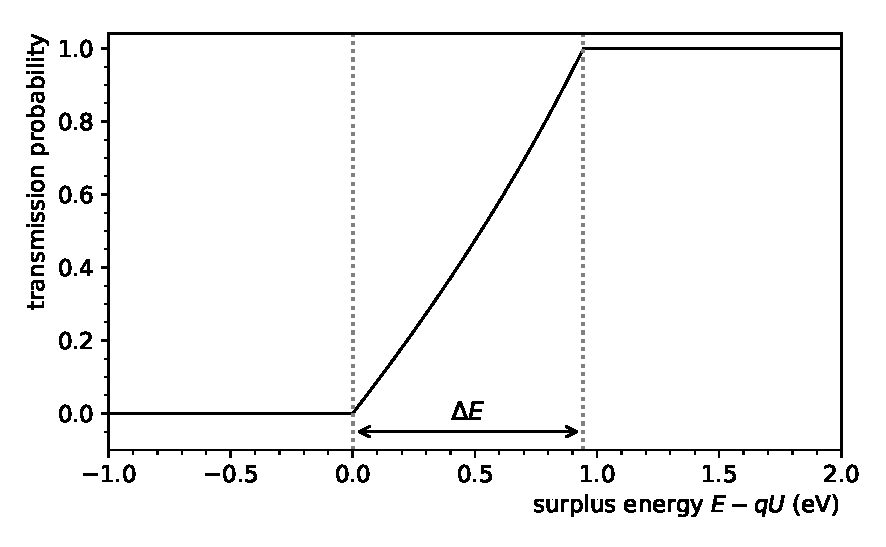
\includegraphics[width=\textwidth]{\currentFigureFolder/transmission.pdf}
	\xcaption{The KATRIN transmission function}{The KATRIN transmission function}{as described by equation \eqref{eq:intSpecModelTransmission}. It denotes the probability for an electron with a kinetic energy $E$ to pass through the spectrometer set to a retarding potential of $U$. The probabilistic treatment of the starting pitch angles of electrons leads to the \gls{mace}-filter width $\Delta E$ with the nominal value of \SI{0.93}{eV^2}~\cite{Angrik:2005ep}. (The transmission function depicted here was calculated using the SSC software framework, see section \ref{sec:statMethodsKaFitSSC}.) }
	\label{fig:intSpecModelTransmission}
\end{figure}
The transmission function denotes the probability of an electron to pass the \gls{mace} filter. It can be characterized by the so-called transmission energy~\cite{Groh2015}
\begin{equation}
\label{eq:intSpecModelTransmissionEnergy}
\Etrans = 
\frac{
	q(U-\Usource)
}{
	1-\sin^2\thetaSource \frac{\Bana}{\Bsource} \frac{\gamma(E)+1}{\gammaAna+1}
}
\fullstop
\end{equation}
where $\gamma(E)$ and $\gammaAna$ denote the relativistic Lorentz factor of the $\upbeta$ electrons with energy $E$ and in the analyzing plane. As the electrons are slowed down substantially by the retarding potential in the spectrometer, it holds $\gammaAna\approx1$. In the following, for ease of notation, also $\Usource=0$ and $\gammaSource=1$ is assumed.

Electrons pass the \gls{mace} filter if their energy $E$ when arriving at the spectrometer surpasses the transmission energy $\EtransPure$, equation~\eqref{eq:intSpecModelTransmissionEnergy}. This condition can be resolved for the starting pitch angle~\cite{Groh2015}
\begin{align}
&E > \Etrans \nonumber \\
\Leftrightarrow \quad
& \thetaSource < \thetaTrans
\coloneqq
\arcsin
\left(\sqrt{
	\frac{E-qU}{E} 
	\frac{\Bana}{\Bsource}
}\right)
\fullstop
\label{eq:intSpecModelTransmissionPitchAngle}
\end{align}
Using equation \eqref{eq:intSpecModelTransmissionPitchAngle}, the transmission function depending on the starting pitch angle and the starting energy of electrons can be formulated as a step function
\begin{equation}
\label{eq:intSpecModelTransmissionStep}
\mathcal{T}(E, qU, \thetaSource) =
\begin{cases}
1 & \text{if } \thetaSource < \thetaTrans \\
0 & \text{otherwise} 
\end{cases}
\fullstop
\end{equation}
Calculating the mean value of this step function with respect to the probabilistic distributed starting pitch angles of $\upbeta$ electrons as described in section~ \ref{sec:intSpecModelResponseConcepts} yields the often quoted KATRIN transmission function~\cite{Angrik:2005ep}
\begin{equation}
\label{eq:intSpecModelTransmission}
	T(E, qU) = 
	\mean{\mathcal{T}(E, qU, \thetaSource)} =
	\begin{cases}
	0 & \text{ if } E < qU \\
	\frac{
		1-\sqrt{
			1-\frac{E-qU}{E} 
			\frac{\Bsource}{\Bana}
		} 
	}{
		1-\sqrt{1-\frac{\Delta E}{E}\frac{\Bsource}{\Bana}}
	}
	& \text{ if } qU < E < qU + \Delta E \\
	1 & \text{ if } qU + \Delta E < E
	\end{cases}
	\comma
\end{equation}
where 
\begin{equation}
	\label{eq:intSpecModelTransmissionMACEFilterWidth}
	\Delta E=E\cdot\Bana/\Bmax
\end{equation}
is the \gls{mace}-filter width as explained in section~\ref{sec:katrinExpSetupSpectrometer}. The transmission function is depicted in figure~\ref{fig:intSpecModelTransmission} for the KATRIN design values. In summary, this section yielded a quantitative treatment of the characteristics of the KATRIN \gls{mace} spectrometer. The following sections are dedicated to the \gls{wgts}.

\subsection{Probability of Electron Scattering within the \glsentryshort{wgts}}
\label{sec:intSpecModelResponseScattering}
This section aims at deriving an expression for the probability $P_l$ of an electron to scatter $l$ times within the \gls{wgts} in a bottom-up approach.

A derivation may start with an expression for the effective column density $\lambda$ an electron passes through: The electron moves on a spiral track due to its cyclotron motion in the magnetic field in the \gls{wgts}. Therefore, when traveling an infinitesimal distance $\d z$ in $z$-direction, it travels a total distance of
\begin{equation}
\label{eq:intSpecModelInfinitesimalElecPath}
\d s = \frac{1}{\cos\thetaSource} \d z 
\fullstop
\end{equation}
(Remarkably, this expression is independent of the electron energy and the magnetic field strength in the \gls{wgts}.)
The effective column density can then be expressed as a path integral over the gas density~$\rho(z)$ from the starting position of the electron to the point where it leaves the \gls{wgts}
\begin{equation}
\label{eq:intSpecModelEffColumnDensity}
\lambda(\zSource,\thetaSource) = 
\int_{\varphi} \rho(\Vec{r})\d s =
\frac{1}{\cos\thetaSource}
\int_{\zSource}^{d/2} \rho(z)\d z
\fullstop
\end{equation}
The expected scattering count then is the product of the effective column density $\lambda(\zSource,\thetaSource)$ and the scattering cross section $\sigma$~\cite{Groh2015}
\begin{equation}
\label{eq:intSpecModelExpectedScatteringCount}
\mu(\zSource, \thetaSource) = \lambda(\zSource,\thetaSource) \sigma \fullstop
\end{equation}
The scattering process fulfills the conditions of a Poisson process, namely scattering once does quasi not influence the probability of an electron to scatter again; the expected scattering count $\mu(\zSource, \thetaSource)$ stays constant (under the assumptions made so far); and it is unlikely for two scatterings to happen within a short distance. Thus, the probability for $l$-fold scattering can be expressed as a Poisson distribution~\cite{Groh2015}
\begin{equation}
\label{eq:intSpecModelNonAveragedScatProbs}
P_l(\zSource, \thetaSource) = 
\frac{
	\mu(\zSource, \thetaSource)^l
}{l!}
\mathrm{e}^{-\mu(\zSource, \thetaSource)} \fullstop
\end{equation}
The mean value with respect to the starting positions and the starting pitch angles can be calculated~\cite{Groh2015}
\begin{equation}
	\label{eq:intSpecModelAveragedScatProbs}
	\bar{P}_l =
	\frac{1}{d}
	\int_{-d/2}^{d/2}
		\frac{1}{1-\cos\thetaMax}
		\int_{0}^{\thetaMax}
			\sin\thetaSource
			P_l(\zSource,\thetaSource)
		\d \thetaSource
	\d \zSource
	\fullstop
\end{equation}
Table~\ref{tab:intSpecModelAveragedScatProbs} lists the numerical evaluation of these averaged scattering probabilities. With these probabilities at hand, the next step is the derivation of the energy an electron looses when scattering.

\begin{table}[ht]
	\centering
	\xcaption{Averaged probability for electron scattering within the \gls{wgts}}{Averaged probability for electron scattering within the \gls{wgts}.}{Listed are the evaluations of equation \eqref{eq:intSpecModelAveragedScatProbs} for the following input parameters:
	A scattering cross section of $\sigma=\SI{3.456e-22}{m^2}$~\cite{Angrik:2005ep},
	a constant gas column density $\rho d = \SI{5e17}{cm^{-2}}$, 
	a \gls{wgts} length of $d=\SI{10.0820}{m}$
	and a maximum acceptance angle of $\thetaMax=\SI{50.7685}{\degree}$.
	The same values can be found in \cite{Groh2015, Kleesiek2014}.}
	\begin{tabular}{cr}
		\toprule
		\makecell[tl]{scattering count $l$} &
		\makecell[tl]{scattering probability\\ according to equation \eqref{eq:intSpecModelAveragedScatProbs}}\\
		\hline
		0 & 41.33\,\SI{}{\percent }\\
		1 & 29.27\,\SI{}{\percent} \\
		2 & 16.73\,\SI{}{\percent} \\
		3 &  7.91\,\SI{}{\percent} \\
		4 &  3.18\,\SI{}{\percent} \\
		\bottomrule
	\end{tabular}
	\label{tab:intSpecModelAveragedScatProbs}
\end{table}

\subsection{Energy Loss of Electrons due to Scattering}
\label{sec:intSpecModelResponseEloss}
\newcommand{\epsCrit}{\epsilon_\mathrm{c}}
\begin{figure}
	\floatbox[{\capbeside
		\captionsetup[capbesidefigure]{}%
		\thisfloatsetup{capbesideposition={left,top}, capbesidewidth=6.4cm}}]{figure}[\FBwidth][][t]
	{
		\xcaption{The energy loss probability density due to electron scattering in the \glsentryshort{wgts}}{The energy loss probability density due to electron scattering in the \glsentryshort{wgts}}{given by equation \eqref{eq:intSpecModelAseevEloss} and determined at the Troitsk experiment~\cite{Aseev2000}. The table below lists the corresponding parameters, where $\epsilon_1$ was fixed and $\epsCrit$  was chosen to make the piece wise defined function continuous.\vspace{2mm}
			\begin{tabular}{cc}
				\toprule
				\makecell[t]{parameter} &
				\makecell[t]{value}\\
				\hline
				$A_1$ & $0.204\pm0.0001$ \\ 
				$A_2$ & $0.0556\pm0.0003$ \\
				$\omega_1$ & \SI{1.85\pm0.02}{eV} \\
				$\omega_2$ & \SI{12.5\pm0.2}{eV} \\
				$\epsilon_1$ & \SI{12.6}{eV} \\
				$\epsilon_2$ & \SI{14.30\pm0.02}{eV} \\
				$\epsCrit$ & \SI{14.09}{eV} \\
				\bottomrule
			\end{tabular}
		}
		\label{fig:intSpecModelAseevEloss}}
	{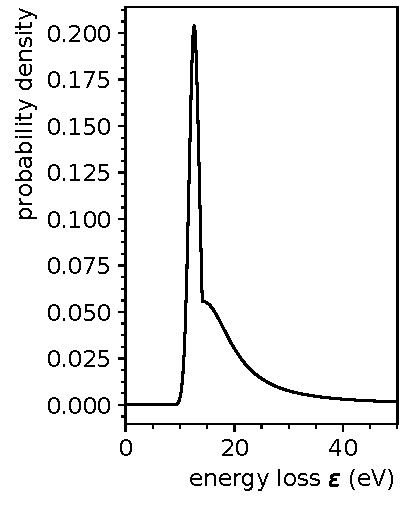
\includegraphics{\currentFigureFolder/eloss.pdf}}
\end{figure}
This section describes the so called ``energy loss function'' $f_l(\epsilon)$. It denotes the probability density for an electron to loose an energy $\epsilon$ when scattering $l$ times. Only the case of inelastic scattering is treated here. For an additional treatment of elastic scattering, which is less likely by one order of magnitude, the reader is referred to~\cite{Kleesiek2019}.

The energy loss function for no scattering is the Dirac delta function~\cite{Kleesiek2019}
\begin{equation}
f_0(\epsilon) = \delta(\epsilon)
\fullstop
\end{equation}

A phenomenological description for 1-fold scattering of electrons from hydrogen isotopologues was derived from data at the Troitsk experiment~\cite{Aseev2000, Abdurashitov2017}
\begin{equation}
\label{eq:intSpecModelAseevEloss}
	f_1(\epsilon) =
	\begin{cases}
		A_1 
		\euler^{ 
			-2\left(
			\frac{\epsilon-\epsilon_1}{\omega_1}
			\right)^2
		}
		&\text{ if } \epsilon < \epsCrit \\
		A_2\frac{
			\omega_2^2
		}{
			\omega_2^2+4(\epsilon-\epsilon_2)^2
		} 
		&\text{ if } \epsilon \geq \epsCrit
	\end{cases}
\end{equation}
Figure~\ref{fig:intSpecModelAseevEloss} depicts this energy loss function. It should be noted, that in the scope of this thesis a more recent preliminary energy loss model derived from a dedicated subgroup of the KATRIN collaboration is investigated in chapter~\ref{sec:katrinEloss}.

For multiple scattering the above function $f_1$ has to be convoluted with itself and the energy loss function becomes~\cite{Kleesiek2019}
\begin{equation}
	\label{eq:intSpecModelConvolutedEloss}
	f_l(\epsilon) = \Conv_{i=0}^{l} f_1(\epsilon)
\end{equation}
where $\conv$ denotes the convolution
\begin{equation}
(f \conv f)(\epsilon) = 
\int_{0}^{\infty}  
	f(\epsilon-\epsilon^\prime)f(\epsilon^\prime)
\d \epsilon^\prime 
\fullstop 
\end{equation}
The energy loss function was the last piece needed to assemble the KATRIN response function. 

\subsection{Assembly of the KATRIN Response Function}
\label{sec:intSpecModelResponseReconciliation}
This section aims at giving an expression for the KATRIN response function. It combines the characteristics of the KATRIN spectrometer and the \gls{wgts}. (It should be noted, that the initially chosen notation here differs slightly from those used in the works~\cite{Groh2015,Kleesiek2019} this derivation is largely based on in order to emphasize dependencies on the starting positions $\zSource$ and pitch angles of electrons $\thetaSource$. However, the final results are reconciled.)

The KATRIN response function in dependence of the starting position and pitch angle of an electron reads 
\begin{equation}
	\label{eq:intSpecModelNonAveragedResponse}
	\mathcal{R}(\Esource, qU, \zSource, \thetaSource) =
	\int_{0}^{\Esource-qU}
	\sum_{l}
	\mathcal{T}(\Esource-\epsilon, qU, \thetaSource) \cdot
	P_l(\zSource, \thetaSource) \cdot
	f_l(\epsilon)
	\d \epsilon
	\fullstop
\end{equation}
where the integral goes over the energy losses, the sum goes over the scattering count, $\mathcal{T}$ denotes the non-averaged transmission function \eqref{eq:intSpecModelTransmission}, $P_l$ the non-averaged scattering probabilities \eqref{eq:intSpecModelNonAveragedScatProbs} and $f_l$ the energy loss function \eqref{eq:intSpecModelConvolutedEloss}. In words, the transmission function is smeared by the energy loss probability density and then a weighted sum is formed over generations of $l$-fold scattered electrons where the weight is the probability to scatter $l$ times.

The mean value of equation \eqref{eq:intSpecModelNonAveragedResponse} with respect to the starting pitch angle as described in section~\ref{sec:intSpecModelResponseConcepts} can be calculated. Also the corresponding integral is swapped with the integral over the energy loss and the sum over the scattering count
\begin{align}
	\label{eq:intSpecModelAveragedResponseIntermediate}
	R(\Esource, qU, \zSource) &= 
	\mean{\mathcal{R}(\Esource, qU, \zSource, \thetaSource)} \nonumber\\ &=
	\int_{0}^{\Esource-qU}
	\sum_{l}
	\int_{0}^{\thetaMax}
	\frac{
		\sin\thetaSource \cdot
		\mathcal{T}(\Esource-\epsilon, qU, \thetaSource) \cdot P_l(\zSource, \thetaSource)
	}{1-\cos\thetaMax}
	\d \thetaSource
	\cdot f_l(\epsilon)
	\d \epsilon
	\fullstop
\end{align}
This expression can be reformulated to have the same form as the non-averaged response function \eqref{eq:intSpecModelNonAveragedResponse}. This means, the product ``transmission function times scattering probability times energy loss function'' can be reestablished, which also reconciles the notation  with the expression given in \cite{Groh2015}. Therefore, the factor $1=\bar{P}_l/\bar{P}_l$ with the averaged scattering probabilities from equation \eqref{eq:intSpecModelAveragedScatProbs} is introduced into equation \eqref{eq:intSpecModelAveragedResponseIntermediate} and the so-called ``detailed transmission function'' $T_l^{\star}$ is defined
\begin{align}
	R(\Esource, qU, \zSource) &=
	\int_{0}^{\Esource-qU}
	\sum_{l}
	\underbrace{
		\int_{0}^{\thetaMax}
		\frac{
			\sin\thetaSource \cdot
			\mathcal{T}(\Esource-\epsilon, qU, \thetaSource) \cdot P_l(\zSource, \thetaSource)
		}{(1-\cos\thetaMax) \cdot \bar{P}_l}
		\d \thetaSource
	}_{
		T_l^{\star}(\Esource-\epsilon,qU,\zSource)
	}
	\cdot \bar{P}_l \cdot f_l(\epsilon)
	\d \epsilon \nonumber \\ &=
	\label{eq:intSpecModelFullResponseIntermediate}
	\int_{0}^{\Esource-qU}
	\sum_{l}
	T_l^{\star}(\Esource-\epsilon,qU,\zSource)
	\cdot \bar{P}_l \cdot f_l(\epsilon)
	\d \epsilon
	\fullstop
\end{align}


The non-averaged transmission function $\mathcal{T}$, equation \eqref{eq:intSpecModelTransmissionPitchAngle},  within $T_l^{\star}$ is a step function with respect to the starting pitch angle $\thetaSource$ of an electron. This allows to adapt the upper integral boundary from $\thetaMax$ to $\thetaTransPure$ when integrating over $\thetaSource$ . Furthermore, in analogy to the KATRIN transmission function from equation~\ref{eq:intSpecModelTransmission}, a distinction of cases avoids imaginary square roots. One obtains the detailed transmission function as given in~\cite{Groh2015,Kleesiek2019}
\begin{equation}
	\label{eq:intSpecModelDetailedTransmission}
	T_l^{\star}(E,qU,\zSource) =
	\begin{cases}
		0 &\text{ if } E < qU \\
		\int_{0}^{\thetaTrans}
		\frac{
			\sin\thetaSource \cdot
			P_l(\zSource, \thetaSource)
		}{(1-\cos\thetaMax) \cdot \bar{P}_l}
		\d \thetaSource
		&\text{ if } qU < E < qU + \Delta E \\
		1 &\text{ if } qU+\Delta E < E
	\end{cases}
	\comma
\end{equation}
where $\thetaTransPure$ denotes the transmission-pitch angle \eqref{eq:intSpecModelTransmissionPitchAngle} and $\Delta E$ the \gls{mace}-filter width \eqref{eq:intSpecModelTransmissionMACEFilterWidth}. Furthermore, it was found, that for $l>3$ scatterings the detailed transmission $T_l^{\star}$ function can be exchanged for the KATRIN transmission function \eqref{eq:intSpecModelTransmission} without making a significant error~\cite{Groh2015}.

\paragraph{Summary}
\begin{figure}
	\centering
	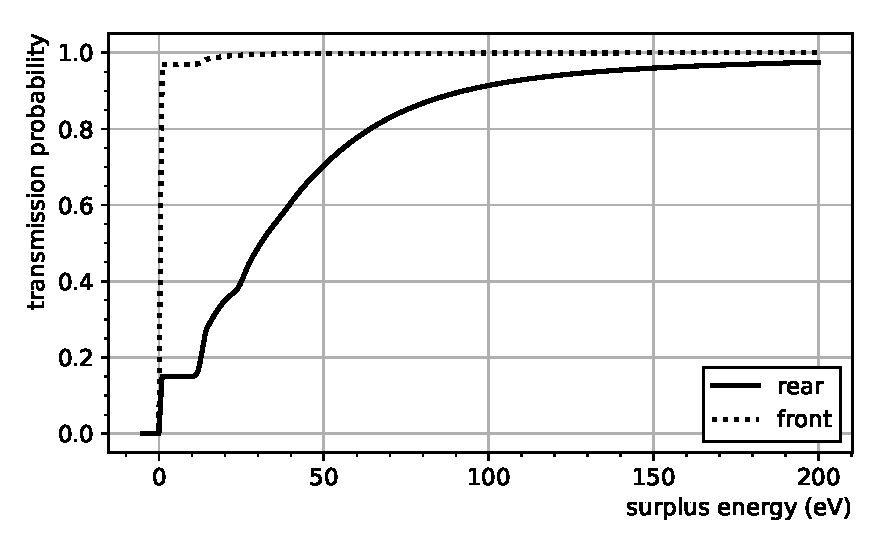
\includegraphics[width=\textwidth]{\currentFigureFolder/response.pdf}
	\xcaption{The KATRIN response function}{The KATRIN response function}{at a retarding voltage of $U=\SI{18545}{V}$. It is depicted for three cases: for electrons starting~\mbox{$\sim\SI{9}{mm}$} from the rear and front of the \gls{wgts} and averaged over all starting positions. The discontinuity in the first derivative of the energy loss function at $\epsCrit=\SI{14.09}eV$ causes kinks. As the energy loss function has an onset at $\epsilon_0\approx\SI{10}{eV}$, the kinks are expected as depicted at approximately $n\cdot\epsilon_0+\epsCrit$ ($n\in\{0,1,\dots\}$) and increasingly smoothed for higher $n$. (Also see figure~\ref{fig:intSpecModelAseevEloss} for the energy loss function.) For unscattered electrons the response function resembles the transmission function. Here, this is approximately the case for electrons starting from the front, as they are unlikely to scatter. That is also, why the plateau of the averaged response function corresponds the averaged probability for electrons not to scatter of \SI{41.33}{\percent} (see table~\ref{tab:intSpecModelAveragedScatProbs}). In contrary, electrons starting from the rear are likely to scatter. Thus, the corresponding response function shows the features of multiple scatterings. For multiple scatterings, the sharp edges of the transmission function are smoothed by the energy loss, which is why only one sharp edge and one plateau is apparent. The depicted response function was calculated using the SSC software framework (see section~\ref{sec:statMethodsKaFitSSC}.), which largely follows equation~\eqref{eq:intSpecModelResponse} and accounts for the $\zSource$ dependency by a discretization (slicing) of the \gls{wgts} volume. For details, the reader is referred to~\cite{Kleesiek2019}.}
	\label{fig:intSpecModelResponse}
\end{figure}
In equation~\ref{eq:intSpecModelFullResponseIntermediate} the KATRIN response function was derived, which reconciles with the expressions given in~\cite{Groh2015,Kleesiek2019}
\begin{equation}
	\label{eq:intSpecModelResponse}
	R(\Esource, qU, \zSource) =
	\int_{0}^{\Esource-qU}
	\sum_{l}
	T_l^{\star}(\Esource-\epsilon,qU,\zSource)
	\cdot \bar{P}_l \cdot f_l(\epsilon)
	\d \epsilon
	\comma
\end{equation}
where $T_l^{\star}$ is the detailed transmission function, equation~\eqref{eq:intSpecModelDetailedTransmission}, $\bar{P}_l$ are the averaged scattering probabilities, equation~\eqref{eq:intSpecModelAveragedScatProbs} and $f_l$ is the energy loss function, equation~\eqref{eq:intSpecModelConvolutedEloss}. The response function denotes the probability of an electron starting with an energy $\Esource$ at a position $\zSource$ to overcome the retarding energy $qU$ and reach the detector. Figure~\ref{fig:intSpecModelResponse} shows the response function for two different starting positions of electrons as well as averaged over all starting positions.

The response function and the differential $\upbeta$ spectrum can now be combined to an expression for the $\upbeta$ electron rate measured by KATRIN. 

\section{Integral Rate}
\label{sec:intSpecModelIntegralRate}
This section aims at deriving an expression for the integral $\upbeta$-electron rate at the KATRIN detector. 

As already mentioned, the response function~\eqref{eq:intSpecModelResponse} depends on the starting position of the electrons. To account for this, the \gls{wgts} can be thought of divided into $n$ slices of width~$w=d/n$ and an averaged response function for the $j$th ($j\in\{0,1,\dots,n-1\}$) slice can be given
\begin{equation}
	R(\Esource,qU,\zSource) \rightarrow
	R_j(\Esource,qU) =
	\int_{-d/2+jw}^{-d/2+(j+1)w}
		R(\Esource,qU,\zSource)
	\d \zSource
	\fullstop
\end{equation}
The integral rate then reads~\cite{Kleesiek2019}
\begin{equation}
	\label{eq:intSpecModelIntegralRate}
	\Gamma(qU) = 
	\frac{1}{2} 
	\sum_{j=0}^{n} N_{j, \mathrm{T}} \cdot
		\int_{qU}^{E_0} 
			\left(\frac{\d \Gamma(\Esource)}{ \d \Esource}\right) \cdot 
			R_j(\Esource, qU) 
		\d \Esource
		\fullstop
\end{equation}
Here, the integral goes over all starting energies that enable electrons to overcome the retarding potential; the sum goes over all slices of the \gls{wgts}; $N_{j, \mathrm{T}}$ is the number of tritium nuclei in the $j$th slice of the \gls{wgts}; and the factor $1/2$ accounts for the fact, that on average only half the $\upbeta$ electrons are emitted towards the detector.

\section{Detector Counts}
This section aims at deriving an expression for the electron counts measured by the KATRIN detector. 

Therefore, the detector efficiency \mbox{$\epsilon_\mathrm{det}\in[0,1]$} has to be taken into account. (For a description, its determination and value see section~\ref{sec:katrinExpSetupDetector}.) Furthermore, the background rate~$\bgRate$ with a nominal value of $\SI{10}{cps}$~\cite{Angrik:2005ep} has to be considered. Also a relative rate factor $\sigAmp=1$ between the background and the $\upbeta$-electron rate is introduced as it can be used in fitting procedures (see section~\ref{sec:statMethodsStandardFit}.) Assuming a measurement time of $t(qU)$ attributed to a retarding energy $qU$, the detector counts are~\cite{Kleesiek2014}
\begin{equation}
\label{eq:intSpecModelDetectorCounts}
	N(qU) = t(qU)\cdot\epsilon_\mathrm{det}\cdot
	\left(
		\sigAmp\cdot \Gamma(qU) + \bgRate
	\right)
	\comma
\end{equation}
where $\Gamma(qU)$ denotes the integral rate~\eqref{eq:intSpecModelIntegralRate}. 

\section{Measurement Time Distribution}
\label{sec:intSpecModelMTD}
KATRIN measures electron counts as described in equation \eqref{eq:intSpecModelDetectorCounts} at a set of retarding energies $\left\{qU_i\right\}$. How much measurement time $t(qU_i)$ is attributed to a certain retarding energy is specified in a \gls{mtd}. The \gls{mtd} influences the experiment's sensitivity to the neutrino mass. An optimal \gls{mtd} balances the following aspects:
\begin{enumerate}
	\item Some measurement time has to be attributed to retarding energies beyond the endpoint of the integral tritium-$\upbeta$ spectrum to determine the background rate. The optimal duration depends on the background rate, but can generally take up a sizable fraction (of order \SI{30}{percent}) of the overall measurement time. ~\cite{Angrik:2005ep}.
	\item Near its endpoint, the shape of the integral tritium-$\upbeta$ spectrum depends most strongly on the neutrino mass. Hence, most measurement time should be attributed to this region~\cite{Angrik:2005ep}.
	\item Retarding voltage bins deeper into the spectrum increase the count rate and hence, lower the statistical uncertainty due to Poisson statistics. Theses measurements mainly determine the endpoint from extrapolating the slope of the integral tritium-$\upbeta$ spectrum~\cite{Angrik:2005ep}.
	\item The theoretical description of the integral tritium-$\upbeta$ spectrum is optimized for the endpoint region. E.\,g.~the molecular final states for $\upbeta$-electron energies \SI{40}{eV} below the endpoint would need further investigation~\cite{Doss:2006}. Hence, deeper scans introduce modeling uncertainties. However, it is expected that continuous modeling efforts decrease these uncertainties as needed.
\end{enumerate}
The KATRIN Design Report~\cite{Angrik:2005ep} suggests 5 \gls{mtd}s for different measurement ranges $[E_0-\alpha\;\SI{}{eV}, E_0 + \SI{5}{eV}]$ with $\alpha \in \{20, 25, 30, 40, 50\}$ and the conclusion that $\alpha=30$ yields the best sensitivity to the neutrino mass.

As an energy-dependent effect is investigated within this thesis, it should be noted, that scans beyond the $\SI{50}{eV}$ range have already been performed and may also be performed again in the future. E.\,g.~searches for sterile neutrinos at the keV-scale would require deeper scans~\cite{Mertens2019}. On top of that, within several measurement campaigns deeper scans were conducted: The \gls{ft} commissioning campaign successfully proved the apparatus functioning. The corresponding \gls{mtd} covered a range starting at $\sim\,E_0-\SI{1.6}{keV}$. The \gls{knm1} is being evaluated during the writing of this thesis. It set out to establish an unprecedented limit on the neutrino mass by $\upbeta$-decay measurements. Its \gls{mtd} starts at $\sim\,E_0-\SI{90}{eV}$, but the analysis range for neutrino mass inference remains still to be determined.

\section{A KATRIN Neutrino Mass Measurement}
\label{sec:intSpecModelNuMassMeasurement}
\begin{figure}
	\centering
	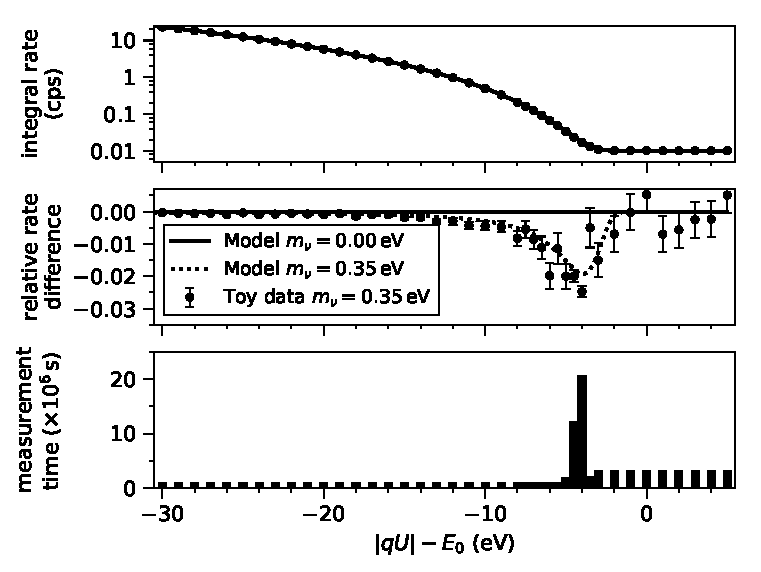
\includegraphics[width=\textwidth]{\currentFigureFolder/neutrinoMassMeasurement.pdf}
	\xcaption{Simulated KATRIN measurement for a non-vanishing neutrino mass.}{Simulated KATRIN measurement for a non-vanishing neutrino mass.}{The top panel shows the measured integral rate $\Gamma$ in dependence of the retarding energy. The center panel shows the relative rate difference for a non-vanishing neutrino mass $\Gamma(\nuMass=\SI{0.35}{eV})/\Gamma(\nuMass=\SI{0}{eV})-1$. The difference is $\sim\SI{2}{\percent}$ at a retarding energy approximately $\SI{4}{eV}$ below the endpoint (simulated as $E_0=\SI{18575}{eV}$). The bottom panel shows the \gls{mtd} where most measurement time is attributed to the most sensitive region. This is also reflected by the uncertainty bars of the toy data. (Adapted from~\cite{SeitzM2019}.)}
	\label{fig:katrinExpNuMassMeasurement}
\end{figure}
In summary, a KATRIN measurement yields a set of electron counts $\{N(qU_i)\}$, equation \eqref{eq:intSpecModelDetectorCounts}, distributed over retarding voltage bins $\{qU_i\}$, where the counts fluctuate statistically~\cite{Angrik:2005ep}. The fluctuation can be assumed to be of Poissonian nature~\cite{Kleesiek2014}. Figure~\ref{fig:katrinExpNuMassMeasurement} shows a KATRIN measurement for an \gls{mtd} starting at $E_0-\SI{30}{eV}$ and a total measurement time of three years. The distortion of the measured integral rate by a non-vanishing neutrino mass can be seen approximately \SI{-4}{eV} below the endpoint $E_0$. This distortion can be used to infer the squared electron antineutrino mass from a KATRIN neutrino mass measurement. Chapter~\ref{sec:statMethods} presents corresponding statistical methods.
    \def\currentRootFolder{chapter/statisticalMethods}
\def\currentFigureFolder{\currentRootFolder/fig}
\newcommand{\dataVec}{\vect{x}}
\newcommand{\paramVec}{\vect{\theta}}
\newcommand{\paramVecShared}{\vect{\theta}_\mathrm{s}}

\newcommand{\nuisanceParamVec}{\vect{\pi}}
\newcommand{\profLikelihood}{L_\mathrm{p}}

\makeatletter
\newcommand{\@giventhatstar}[2]{\left(#1\;\middle|\;#2\right)}
\newcommand{\@giventhatnostar}[3][]{#1(#2\;#1|\;#3#1)}
\newcommand{\giventhat}{\@ifstar\@giventhatstar\@giventhatnostar}
\makeatother

\newcommand{\Nobsi}{N_{\mathrm{obs,}i}}
\newcommand{\Ntheoi}{N_{\mathrm{theo,}i}}

\newcommand{\totUncert}{\sigma(\nuMass^2)}
\newcommand{\statUncert}{\sigma_\mathrm{stat}(\nuMass^2)}
\newcommand{\sysUncert}{\sigma_\mathrm{sys}(\nuMass^2)}
\newcommand{\statUncertTDR}{\sigma_\mathrm{stat}^\mathrm{TDR}(\nuMass^2)}
\newcommand{\sysUncertTDR}{\sigma_\mathrm{sys}^\mathrm{TDR}(\nuMass^2)}



\newacronym{mle}{MLE}{maximum likelihood estimator}
\chapter{Statistical Methods and Neutrino Mass Inference at KATRIN}
\label{sec:statMethods}
The best estimator for the neutrino mass $m_\nu$ alongside with an uncertainty or an upper limit will be retrieved by comparing the output of the KATRIN measurement with theoretical predictions within the process of parameter inference. This chapter reviews a selection of statistical approaches suitable in relation to the KATRIN experiment.

Section~\ref{sec:statMethodsMLE} outlines the principle of the \glsentryfull{mle}. Section~\ref{sec:statMethodsKATRINLikelihood} relates the principle of the \glsentryshort{mle} to a KATRIN measurement and neutrino mass inference. Section~\ref{sec:statMethodsStandardFit} introduces the formalism of a nominal neutrino mass fit at KATRIN. Section~\ref{sec:statMethodsUncertaintyIntervals} reviews the concept of uncertainty intervals and how confidence intervals can be extracted from the likelihood. Section~\ref{sec:statMethodsKaFitSSC} introduces the software framework that was used within this thesis. Section~\ref{sec:statMethodsKatrinSensitivity} relates the principle of uncertainty to neutrino mass inference and explains the origin of the often quoted $\SI{200}{meV}$ (\SI{90}{\percent} C.L.) KATRIN sensitivity.

\section{Maximum Likelihood Estimation}
\label{sec:statMethodsMLE}
The likelihood is the probability of a measurement outcome given a hypothesis. A hypothesis depending on a parameter vector $\paramVec$ is called a composite hypothesis. A measurement outcome can be quantified by a vector of observed values $\dataVec$. The probability $P$ of $\dataVec$ given a hypothesis in dependence of $\paramVec$ is called the likelihood function~\cite{ReviewOfParticlePhysics}
\begin{equation}
	L(\paramVec) = P\giventhat{\dataVec}{\paramVec}
	\fullstop
\end{equation}
If $p$ denotes the probability for one observed value $x_i$ in $\dataVec$, then the likelihood function can be written as a product~\cite{ReviewOfParticlePhysics}
\begin{equation}
	L(\paramVec) = \prod_{i} p\giventhat{x_i}{\paramVec}
	\fullstop
\end{equation}
The parameter vector $\hat{\paramVec}$ that maximizes the likelihood function is called the \gls{mle} for the true values of $\paramVec$.

\section{The Likelihood of a KATRIN Measurement}
\label{sec:statMethodsKATRINLikelihood}
The \gls{mle}-method can be applied to a KATRIN measurement as follows: The data vector is given by a set of $n$ electron counts $\left\{\Nobsi\right\}$ measured at different retarding potentials $\left\{qU_i\right\}$. The hypothesis is that these counts follow a Poisson distribution with predicted expected electron counts $\left\{\Ntheoi\right\}$ as per equation \eqref{eq:intSpecModelDetectorCounts}~\cite{Kleesiek2014}. For sufficiently high counts ($>25$~\cite{Kleesiek2019}) the Poisson distribution can be approximated by a Gaussian distribution $\mathcal{N}(x,\mu, \sigma)$ with mean $\mu=\Ntheoi(\paramVec)$ and standard deviation $\sigma=\sqrt{\Nobsi}$. The likelihood function then reads~\cite{Kleesiek2014}
\begin{equation}
	\label{eq:KATRINlikelihood}
	L(\paramVec) = \prod_{i}^{n} \mathcal{N}\left(
		x=\Nobsi,
		\mu=\Ntheoi(\paramVec),
		\sigma=\sqrt{\Nobsi}
	\right)
	\fullstop
\end{equation}
Commonly, instead of maximizing the likelihood function, its negative logarithm is minimized and a factor 2 is introduced~\cite{ReviewOfParticlePhysics}. This yields
\begin{equation}
	\label{eq:statMethodsKatrinChi2}
	-2\ln L(\paramVec) = \chi^2(\paramVec) = \sum_i^n
		\left( 
			\frac{\Nobsi-\Ntheoi(\paramVec)}{\sqrt{\Nobsi}}
		\right)^2
		 + \mathrm{constants}
		\fullstop
\end{equation}
The minimization of equation~\eqref{eq:statMethodsKatrinChi2} yields the \gls{mle} estimator $\hat{\paramVec}$ for $\paramVec$.

Equation~\eqref{eq:statMethodsKatrinChi2} is a sum of $n$ standard normal distributed random variables. Hence, evaluated at the \gls{mle}, this chi-square expression $\chi^2(\hat{\paramVec})$ follows the Pearson's chi-square statistic with $n-\mathrm{dim}\paramVec$ degrees of freedom. Accordingly, the value $\chi^2(\hat{\paramVec})$ is a measure for the goodness-of-fit~\cite{ReviewOfParticlePhysics}. In conclusion, equation~\eqref{eq:statMethodsKatrinChi2} can be used for neutrino mass inference via the maximum likelihood method.

\section{A Nominal KATRIN Neutrino-Mass Fit}
\label{sec:statMethodsStandardFit}
In regard to a KATRIN neutrino mass measurement, the parameter of interest in the parameter vector $\paramVec$ is the squared neutrino mass $m_\nu^2$. Furthermore, $\paramVec$ typically comprises the endpoint of the tritium-$\upbeta$ spectrum $E_0$, equation~\eqref{eq:intSpecModelDiffSpecNeutrinoEnergy}, an overall normalization factor for the $\upbeta$-electron counts $\sigAmp$ and the background rate $\bgRate$~\cite{Kleesiek2014,Angrik:2005ep}, that are treated as nuisance parameters. For the latter two see equation~\eqref{eq:intSpecModelDetectorCounts}. Hence, in order to infer the neutrino mass, the four-dimensional likelihood has to be minimized. Following this procedure with simulated data enables the determination of KATRIN's sensitivity (see subsequent section~\ref{sec:statMethodsKatrinSensitivity}).

\section{Uncertainty Intervals}
\label{sec:statMethodsUncertaintyIntervals}
The presented maximum likelihood method (section~\ref{sec:statMethodsMLE}) provides point estimates $\hat{\paramVec}$. However, additional information can be provided by interval estimates. There are two main approaches to statistical inference, which may be called Bayesian and frequentist~\cite{ReviewOfParticlePhysics}. They differ in their interpretation of probability, which becomes especially evident by the interval estimates associated with the two approaches: Credible and confidence intervals. Both interval types can be given with reference to quantiles of the Gaussian distribution. E.\,g.~the 1- and 2-$\sigma$ levels define \SI{68}{\percent} and \SI{95}{\percent} intervals. The following two sections~\ref{sec:statMethodsUncertaintyIntervalsCredible} and~\ref{sec:statMethodsUncertaintyIntervalsConfidence} explain the matter in more detail.

\subsection{Bayesian Credible Intervals}
\label{sec:statMethodsUncertaintyIntervalsCredible}
The likelihood $L\giventhat{\dataVec}{\paramVec}$ is a probability distribution for the data $\dataVec$ given the parameters $\paramVec$. The likelihood can be transformed into a probability density for the parameters $\paramVec$ by multiplication with a prior distribution $\pi(\paramVec)$ and normalization to one using Bayes theorem. One obtains the posterior distribution~\cite{ReviewOfParticlePhysics}
\begin{equation}
\label{eq:statMethodsPosterior}
	P\giventhat{\paramVec}{\dataVec} = 
		\frac{
			L\giventhat{\dataVec}{\paramVec}\pi(\paramVec)
		}{
			\int L\giventhat{\dataVec}{\paramVec^\prime}\pi(\paramVec^\prime) \d\paramVec^\prime
		}
	\fullstop
\end{equation}
Credible regions, in which the true parameters lie with a certain probability can be extracted. When $\paramVec$ is one dimensional a credible region is also called a credible interval. 

\subsection{Frequentist Confidence Intervals}
\label{sec:statMethodsUncertaintyIntervalsConfidence}
This section first gives definitions for the terms ``confidence interval'', ``coverage probability'' and ``confidence level''. It is explained, how confidence intervals can be extracted from a likelihood on the basis of these definitions. This approach was applied within the scope of this thesis in order to study the impact of model uncertainties on KATRIN's sensitivity in chapter~\ref{sec:katrinEloss}.

In frequentist statistics, probability is interpreted as the frequency of the outcome of a repeatable experiment. The boundary of a confidence region is given by a function of the data. There is some freedom of choice for the corresponding function. It should be noted that in this sense, the term confidence region is somewhat ``unqualified''~\cite{ReviewOfParticlePhysics}. But it obtains a deeper meaning in combination with a coverage probability. First, it should be noted that the boundary of the confidence region would fluctuate if one were to repeat the experiment many times. One would obtain an ensemble of confidence regions. The coverage probability $\alpha$ refers to the fraction of regions in such an ensemble that contains the true parameter values~$\paramVec_\mathrm{T}$\cite{ReviewOfParticlePhysics}. If an ensemble of confidence regions covers the true parameter values~$\paramVec_\mathrm{T}$ at least a fraction of $\alpha$ times, the confidence interval is understood to have a confidence level of $\alpha$~\cite{ReviewOfParticlePhysics}. When $\paramVec$ is one dimensional a corresponding confidence region is called a confidence interval. 


In a practical context, a prescription is required on how to construct confidence intervals of a eligible confidence level. The Neyman construction~\cite{Neyman1937} or the unified approach by Feldman and Cousins~\cite{Feldman1998} are such prescriptions.

A further method of constructing confidence intervals is to consider a test (see hypothesis testing in~\cite{ReviewOfParticlePhysics}) of the hypothesis that the parameter values $\paramVec$ have the true values $\paramVec_\mathrm{T}$~\cite{ReviewOfParticlePhysics}. In this construction the choice of test to be used is free. One possibility is a test statistic based on the likelihood ratio between the \gls{mle} $\hat{\paramVec}$ and $\paramVec$~\cite{ReviewOfParticlePhysics}
\begin{equation}
	\label{eq:statMethodsLikelihoodRatio}
	\lambda(\paramVec) =
	\frac{L(\paramVec)}{L(\hat{\paramVec})}
	\fullstop
\end{equation}
In the case of a construction via a hypothesis test, all parameter values $\paramVec$ are excluded from the confidence interval of level $\alpha$ that are rejected by the test with a significance of $\alpha$~\cite{ReviewOfParticlePhysics}.

If the likelihood follows the form of a multivariate Gaussian distribution in $\paramVec$, then the above test statistic~\eqref{eq:statMethodsLikelihoodRatio} can be evaluated and the hyper surface defined by
\begin{equation}
	\label{eq:statMethodsConfidenceContour}
	\ln L(\paramVec) = 	\ln L(\hat{\paramVec}) - \frac{s^2}{2}
\end{equation}
encloses a $s$-$\sigma$ confidence region for $\paramVec$~\cite{ReviewOfParticlePhysics}. (Here, $s$-$\sigma$ denotes the corresponding quantile of a Gaussian distribution.) 

It should be noted that the extraction of confidence intervals from the KATRIN likelihood requires its extrapolation to nonphysical negative squared neutrino masses~\cite{Kleesiek2014} - a complication that can be avoided when using Bayesian methods.

In conclusion, in this section a constructive approach has been presented, that enables the extraction of confidence regions for the parameters of a KATRIN measurement from the KATRIN likelihood. An extension of this formalism (namely, the profile likelihood method) finds application in the scope of this thesis in chapter~\ref{sec:katrinEloss}.

\section{The KaFit and SSC Software Frameworks}
\label{sec:statMethodsKaFitSSC}
With respect to neutrino mass inference at KATRIN two formalisms have been presented: the model for a KATRIN neutrino mass measurement in chapter~\ref{sec:intSpecModel} and a statistical framework for parameter inference within the current chapter~\ref{sec:statMethods}.

The two formalisms are implemented within two modules of the ``KATRIN Analysis and Simulations Package'' (KASPER)~\cite{Kasper}:\mynobreakpar
\begin{enumerate}
	\item The \textbf{\glsentryfull{ssc}}~\cite{SSC} module implements the formulas for the differential and integrated spectrum calculations. Therefore, it follows the formulas given in chapter~\ref{sec:intSpecModel}. Additionally, it also includes aspects beyond the given description, such as the gas dynamics within the \gls{wgts}~\cite{Hoetzel2012, Groh2015, Kleesiek2019, Kaefer2012}.
	\item The \textbf{KaFit}~\cite{KaFit} module translates the $\upbeta$ spectrum calculated by \glsentryshort{ssc} into expected detector counts. Furthermore, KaFit implements several statistic tools tailored to the KATRIN experiment. One of which is the extraction of confidence intervals according to the profile likelihood method (see section~\ref{sec:statMethodsUncertaintyIntervalsConfidence}), which is of importance in the scope of this thesis. The actual minimization and profiling are done by the interfaced MINUIT2 and MINOS package from the ROOT\footnote{\url{http://root.cern.ch/}}~\cite{ANTCHEVA2009} analysis framework~\cite{Kleesiek2014}.
\end{enumerate}

Both packages were used and extended to allow for the analysis done within the scope of this thesis as will be explained in chapters~\ref{sec:energyDepScat} and~\ref{sec:katrinEloss}.

\section{KATRIN's Sensitivity to the Electron Antineutrino Mass}
\label{sec:statMethodsKatrinSensitivity}
This section explains the origin of the often quoted KATRIN design sensitivity to the neutrino mass of $\SI{200}{meV}$\,(\SI{90}{\percent} C.L.). First, a definition of the sensitivity is given in section~\ref{sec:statMethodsSensitivtyDef}. Then, section~\ref{sec:statMethodsSensitivtyFromEnsemble} and~\ref{sec:statMethodsSensitivtyFromProileLikelihood} show how this definition was applied by different works to deduce KATRIN's sensitivity.

\subsection{Definition and Construction of KATRIN's Sensitivity}
\label{sec:statMethodsSensitivtyDef}
\begin{figure}
	\centering
	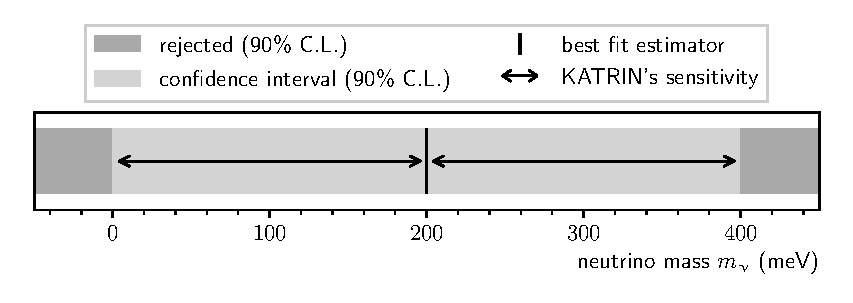
\includegraphics[width=\textwidth]{\currentFigureFolder/sensitivityIllustration.pdf}
	\xcaption{Illustration of KATRIN's sensitivity to the neutrino mass}{Illustration of KATRIN's sensitivity to the neutrino mass.}{The graph illustrates KATRIN's sensitivity of~\SI{200}{meV}~\cite{Angrik:2005ep} as per equation~\eqref{eq:statMethodsSensitivity}. It shows a hypothetical measurements of to the neutrino mass with a symmetric confidence interval \mbox{(\SI{90}{\percent} C.L.)} centrally located around the best fit estimator. If such a classical confidence interval is constructed, KATRIN can reject the null hypothesis of a vanishing neutrino mass at \mbox{\SI{90}{\percent} C.L.} if it estimates a neutrino mass of at least~\SI{200}{meV}.}
	\label{fig:statMethodsSensitivity}
\end{figure}

KATRIN's sensitivity can be understood as half the width of a symmetric and central confidence interval (\SI{90}{\percent} C.L.) for the neutrino mass obtained from a KATRIN neutrino mass measurement. As such it can be constructed from a 1-$\sigma$ uncertainty $\totUncert$ on the squared neutrino mass~\cite{Angrik:2005ep}
\begin{equation}
\label{eq:statMethodsSensitivity}
S_{\nuMass}(\SI{90}{\percent}) = \sqrt{1.645\cdot\totUncert}
\comma
\end{equation}
where the factor 1.645 translates the $\SI{68.3}{\percent}$ interval into a $\SI{90}{\percent}$ interval.

In other words, KATRIN's sensitivity to the neutrino mass can be understood as the minimal neutrino mass that has to be inferred from a KATRIN neutrino mass measurement to exclude the null hypothesis of a vanishing neutrino mass~\cite{Kleesiek2014} when constructing a symmetric and central confidence interval (\SI{90}{\percent} C.L.). Figure~\ref{fig:statMethodsSensitivity} illustrates this statement.

For a more comprehensive picture, where not only a symmetric and central confidence interval is considered, but also the unified approach according to Feldmann and Cousins as well as Bayesian statistics, the reader is referred to~\cite{Kleesiek2019}.

\subsection{Sensitivity from Simulated Ensembles}
\label{sec:statMethodsSensitivtyFromEnsemble}
In the KATRIN Design Report the sensitivity to the neutrino mass was evaluated using ensemble tests. An ensemble of many KATRIN measurements was simulated (see section~\ref{sec:intSpecModelNuMassMeasurement} on how such a simulation can be conducted) with a true neutrino mass of \SI{0}{eV}. From each simulated measurement the squared neutrino mass was inferred in a standard KATRIN four-parameter fit (see section~\ref{sec:statMethodsStandardFit}). Probability was interpreted as the frequency of an outcome of such a fit. The central 1-$\sigma$ interval of the obtained ensemble of squared neutrino masses was taken as the statistical uncertainty on the squared neutrino mass~\cite{Angrik:2005ep}
\begin{equation}
	\statUncertTDR = \SI{0.018}{eV^2}
\end{equation}
A systematic uncertainty was estimated to be approximately \SI{0.01}{eV}. Due to the early stage of the experiment the systematic uncertainty was conservatively enlarged to a systematic budget at approximately the same scale as the statistical uncertainty~\cite{Angrik:2005ep}
\begin{equation}
	\sysUncertTDR = \SI{0.017}{eV^2}
\end{equation}
Adding the statistic and systematic uncertainty quadratically and applying the definition~\eqref{eq:statMethodsSensitivity} yields KATRIN's design sensitivity~\cite{Angrik:2005ep}
\begin{equation}
	\label{eq:statMethodsSensitivityDesignReport}
	S_{\nuMass}^{\mathrm{TDR}}(\SI{90}{\percent}) = 
	\sqrt{1.645\cdot
		\sqrt{
		\statUncertTDR^2+\sysUncertTDR^2
	}}
	\approx \SI{200}{meV}
	\fullstop
\end{equation}
The corresponding investigations were redone in the scope of several works. Table~\ref{tab:statMethodsSensitivityFromEnsembleTests} lists selected results.
\begin{table}[tb]
	\centering
	\xcaption{KATRIN's sensitivity to the neutrino mass from ensemble tests}{KATRIN's sensitivity to the neutrino mass from ensemble tests.}{The table lists KATRIN's sensitivity~$S_{\nuMass}(\SI{90}{\percent})$ as defined by equation~\eqref{eq:statMethodsSensitivity}. Several works reevaluated the statistical uncertainty according to experimental and theoretical progress. For each reevaluation a systematic uncertainty of $\sysUncert = \SI{0.017}{eV^2}$ was assumed. A value derived from an ensemble test is a random variable. Corresponding uncertainty intervals are reprinted where originally stated.}
	\begin{tabular}{lrlr}
		\toprule
		\makecell[t]{$\statUncert$ (\SI{}{eV^2})} & 
		\makecell[t]{$S_{\nuMass}(\SI{90}{\percent})$ (\SI{}{meV})} & 
		\makecell[t]{comment} &
		\makecell[t]{reference}
		\\
		\hline
		0.018 & 200 & design value & \cite{Angrik:2005ep} \\
		$0.0165\pm0.0001$ & 198 & updated $\upbeta$-spectrum calculation & \cite{Hoetzel2012} \\
		$0.0162\pm0.0001$ & 197 & further updated $\upbeta$-spectrum calculation & \cite{Kleesiek2014} \\
		0.01490 & 193 & optimized \gls{mtd} & \cite{Kleesiek2014} \\
		\bottomrule
	\end{tabular}
	\label{tab:statMethodsSensitivityFromEnsembleTests}
\end{table}
\subsection{Sensitivity from  the Profile Likelihood Method}
\label{sec:statMethodsSensitivtyFromProileLikelihood}
In the scope of this thesis, the sensitivity on the neutrino mass as obtained by the profile likelihood method is of importance. (See chapter~\ref{sec:katrinEloss} for a description and application of the profile likelihood method.) In this regard, previous results from~\cite{Kleesiek2014} based on the profile likelihood method are shortly reviewed here. Two uncertainties were obtained for two different~\gls{mtd}s in a KATRIN standard 4-parameter fit (see section~\ref{sec:statMethodsStandardFit}). The first \gls{mtd} had been specially optimized with regard to KATRIN's sensitivity and the resulting statistical uncertainty is $\statUncert=\SI{0.01494}{eV^2}$. For the second result the nominal \gls{mtd} from the KATRIN Design Report was used as introduced in section~\ref{sec:intSpecModelMTD}. The corresponding profile likelihood was plotted and $\statUncert$ can be extracted to be between \SIrange[range-phrase=--]{0.0155}{0.0165}{eV^2}. Both results are in agreement on the $10^{-3}$ level with the results from ensemble tests (see~\cite{Kleesiek2014} in table~\ref{tab:statMethodsSensitivityFromEnsembleTests}). This is an indicator for the general validity of the profile likelihood method in the context of a KATRIN measurement. A more detailed discussion on the matter is given in chapter~\ref{sec:katrinEloss}.
    \def\currentRootFolder{chapter/energyDependentCrossSec}
\def\currentFigureFolder{\currentRootFolder/fig}
\newcommand{\sigmaInel}{\sigma_\mathrm{inel}}
\newcommand{\sigmaAvg}{\sigma_\mathrm{avg}}

\newcommand{\qUmin}{qU_\mathrm{min}}

\newcommand{\Ekin}{E_\mathrm{kin}}
\newcommand{\nSource}{n_\mathrm{S}}
\newacronym{standardmodel}{SM}{Standard Model of Particle Physics}
\newacronym{lep}{LEP}{Large Electron Positron Collider}
\newacronym{ssm}{SSM}{standard solar model}
\chapter{Energy-Dependence of the Cross Section for Inelastic Electron-Scattering within the \glsentryshort{wgts}}
\label{sec:eDepScatCrossSec}
The probability of an electron to scatter when traveling through the \gls{wgts} can be characterized by the total scattering cross section $\sigma_\mathrm{tot}$. Two types of scatterings can be distinguished: elastic and inelastic scattering. The cross section for elastic scattering is smaller than the one for inelastic scattering by one order of magnitude~\cite{Kleesiek2019}. This chapter focuses on inelastic scattering and neglects elastic scattering. Within this chapter, the cross section for electrons scattering inelastically off tritium molecules is just denoted as ``cross section'' and with the symbol $\sigma$. For ease of notation and reading, the adjective ``inelastic'' and an index such as ``inel'' is omitted where the context allows it unambiguously.

The cross section depends on the energy of the incident electrons: $\sigma \equiv \sigma(E)$. This dependence has been neglected in the formal modeling of a KATRIN measurement described in chapter~\ref{sec:intSpecModel}. This chapter investigates effects related to the incorporation of the energy-dependence. Section~\ref{sec:eDepScatCrossSecSources} lists cross section values and formulae from different sources and relates them to each other. Section~\ref{sec:eDepScatCrossSecModelPoisson} extends the mathematical formalism for a KATRIN measurement in order to incorporate the energy-dependence of the scattering cross section. However, an approximation is made. It is neglected, that an electron that scatters loses energy and becomes more likely to scatter again. This issue is addressed in section~\ref{sec:eDepScatCrossSecModelExtended}. Section~\ref{sec:eDepScatCrossSecNuMassInf} discusses the energy-dependence of the scattering cross section within the context of neutrino mass inference using the approximated model. And section~\ref{sec:eDepScatCrossSecConclusion} concludes and offers an outlook.


\section{Cross Section for Electrons Scattering off Molecular Hydrogen Isotopologues}
\label{sec:eDepScatCrossSecSources}
The goal of this thesis is to investigate to what extend it is important, that the cross section value is not constant but varies with the energy of the incident electrons. In that regard, a formula by~\cite{Liu1987} is used, that is derived from first principles and denotes the energy-dependent cross section for electrons scattering off hydrogen molecules. This was found to be a feasible approach for the stated goal - at least for first investigations. In section~\ref{sec:eDepScatCrossSecSourcesTheory}, this formula by~\cite{Liu1987} is reviewed. For electrons with an energy of $\Esource=\SI{18.6}{keV}$, its application yields 
\begin{equation}
	\label{eq:eDepScatCrossSecSourcesCrossSecLiuAtEndpoint}
	\sigma(\SI{18.6}{keV}) = \SI{3.667e-22}{m^2}
	\fullstop
\end{equation}
The formula is in agreement on at least the $10^{-1}$ level with recent, preliminary estimations obtained through data taken at the KATRIN experiment for electrons scattering off tritium molecules. This hints at its applicability, which is of importance in the light of the following paragraph.

The situation regarding cross section values is not without a certain intricacy. The following list gives an introduction to the matter that shall serve as guidance for the reader:\mynobreakpar
\begin{enumerate}
	\item In this work, a theoretical cross section for electrons scattering off hydrogen molecules is used. During a KATRIN neutrino mass measurement, the \gls{wgts} is envisaged to be filled with gas of \SI{95}{\percent} tritium purity~\cite{Angrik:2005ep}. In that regard, the scattering off tritium molecules is of importance with respect to the KATRIN experiment. How the formulas for scattering off hydrogen molecules can be transformed to tritium molecules is under investigation at the time of writing this thesis. Once, this process is completed, the study presented in this thesis might have to be repeated.
	\item The cross section for electrons with an energy of \SI{18.6}{keV} scattering off tritium molecules was measured at the neutrino mass experiment in Troitsk to be~\cite{Aseev2000}
	\begin{equation}
		\sigma(\SI{18.6}{eV}) = \SI{3.40\pm0.07e-22}{m^2}
		\fullstop
	\end{equation}
	This value differs by approximately \SI{8}{\percent} and 4 standard deviations from the theoretical value given above in equation~\eqref{eq:eDepScatCrossSecSourcesCrossSecLiuAtEndpoint}.
	\item The KATRIN Design Report lists a reference value~\cite{Angrik:2005ep}
	\begin{equation}
	\label{eq:eDepScatCrossSecSourcesCrossSecTDR}
	\sigma_\mathrm{TDR} = \SI{3.456e-22}{m^2}
	\fullstop
	\end{equation}
	This value also differs significantly from the theoretical value given above in equation~\eqref{eq:eDepScatCrossSecSourcesCrossSecLiuAtEndpoint}. To further complicate the matter, comparability with former results is of importance in the scope of this thesis and several former works are based on $\sigma_\mathrm{TDR}$. Section~\ref{sec:eDepScatCrossSecSourcesChoice} explains why the value of $\sigma_\mathrm{TDR}$ might be erroneous and how this issue is addressed in this work.
\end{enumerate}

\subsection{Theoretical Cross Section Formulae}
\label{sec:eDepScatCrossSecSourcesTheory}
An expression for the inelastic cross section for electrons scattering off hydrogen molecules can be found in~\cite{Liu1973}. Two expressions are given: one for relativistic incident electrons and one for non-relativistic incident electrons. In regard to KATRIN, the energies of $\upbeta$~electrons from tritium $\upbeta$~decay are relevant. The maximum relativistic $\beta$~factor of electrons from tritium $\upbeta$~decay is
\begin{align}
\beta(E, m) &= 
\sqrt{
	1-\frac{1}{
		(\frac{E}{m}+1)^2
	}
} \label{eq:eDepScatCrossSecSourcesCrossSecBetaFactor} \\
\Rightarrow\beta_\mathrm{max, T} &= 
\beta(E\approx\SI{18.6}{keV}, m_\elecIndex\approx\SI{511}{keV})\approx0.26 
\fullstop
\end{align}
Traveling at approximately a forth of the speed of light, the $\upbeta$~electrons are assumed to behave non-relativisticly. Then, the given expression for the energy-dependent cross section is~\cite{Liu1973}
\begin{equation}
\label{eq:eDepScatCrossSecSourcesCrossSecLiu}
\sigma(E) =  
(4 \pi a_0^2) \cdot
\left(\frac{T(E)}{R}\right)^{-1} \cdot
\left[
C_1 \cdot \ln{\left(\frac{T(E)}{R}\right)} + C_2
\right]
\end{equation}
with the Bohr radius\footnote{Bohr radius $a_0=\SI[separate-uncertainty=false]{0.529 177 210 67(12)e-10}{m}$~\cite{ReviewOfParticlePhysics}} $a_0$, 
the Rydberg energy\footnote{Rydberg energy $R=\SI[separate-uncertainty=false]{13.605 693 009(84)}{eV}$~\cite{ReviewOfParticlePhysics}} $R$ and two constants $C_1$ and $C_2$. The later two depend on the hydrogen isotopologue. Different values are stated in different works for scattering off hydrogen molecules
\begin{subequations}
\label{eq:eDepScatCrossSecSourcesCrossSecLiuConstants}
\begin{align}
C_1 &= 1.5487 &&\text{\cite{Liu1973}}
\label{eq:eDepScatCrossSecSourcesCrossSecLiuConstantsC1}
\comma\\[10pt]
C_2 &= 2.2212\pm0.0434 &&\text{\cite{Liu1973}}
\label{eq:eDepScatCrossSecSourcesCrossSecLiuConstantsC2Uncert}
\comma\\
C_2 &= 1.53 &&\text{\cite{Gerhart1975}}
\comma\\
C_2 &= 2.4036 &&\text{\cite{Liu1987}}
\label{eq:eDepScatCrossSecSourcesCrossSecLiuConstantsC2}
\fullstop
\end{align}
\end{subequations}
The latest of these references,~\cite{Liu1987}, acknowledges that the listed values for $C_2$ are not compatible.

Furthermore, in equation~\eqref{eq:eDepScatCrossSecSourcesCrossSecLiu}, $T$ denotes the non-relativistic kinetic energy\footnote{I would like to thank Dr.~F. Glück for pointing this out. Also see~\cite{INOKUTI1971} for notations with regard to Bethe theory in scattering processes.} using the velocity $v$ and the electron rest mass $m_\elecIndex$
\begin{align}
	\label{eq:eDepScatCrossSecSourcesCrossSecNonRelEnergy}
	T  &= \frac{1}{2} m_\elecIndex v^2 = 
	\frac{1}{2} m_\elecIndex  c^2  \frac{v^2}{c^2} \nonumber \\
	&\equiv T(E) = \frac{1}{2} m_\elecIndex  c^2  \beta(E, m_\elecIndex)^2
\end{align}
with $\beta(E, m_\elecIndex)$ as in equation~\eqref{eq:eDepScatCrossSecSourcesCrossSecBetaFactor}\footnote{This thesis uses natural units. However, for clarity, it makes sense to explicitly state the speed of light $c$ in this particular case.}. This formula is valid in the center-of-mass frame of the colliding system of the electron and the hydrogen molecule. As the molecule is significantly heavier than an electron, the center of mass-frame-was assumed to be the rest frame of the molecule. Also, relative movements due to the gas flow and thermal motion in the \gls{wgts} were neglected.

In the scope of this thesis, equation~\eqref{eq:eDepScatCrossSecSourcesCrossSecLiu} with $C_2$ from~\cite{Liu1987} (as it is the most up-to-date of the listed ones) is used to include the energy-dependence of the cross section into the mathematical formalism of a KATRIN neutrino mass measurement.

As already mentioned, \cite{Liu1973} also states a formula for incident electrons with relativistic energies, which is reprinted here for completeness
\begin{equation}
	\label{eq:eDepScatCrossSecSourcesCrossSecLiuRelativistic}
	\sigma(E) =  
	(4 \pi a_0^2) \cdot
	\left(\frac{T(E)}{R}\right)^{-1} \cdot
	\left[
	1.5487 \cdot \ln{\left(\frac{\beta(E,m_\elecIndex)}{1-\beta(E,m_\elecIndex)^2}\right)} + 17.4615
	\right]
	\fullstop
\end{equation}
The quantities $T(E)$, $R$ and $a_0$ match the once in equation~\eqref{eq:eDepScatCrossSecSourcesCrossSecLiu} and $\beta(E, m_\elecIndex)$ follows equation~\eqref{eq:eDepScatCrossSecSourcesCrossSecBetaFactor}. For energies below $\SI{18.6}{keV}$ the difference of the formula for relativistic (eq.~\ref{eq:eDepScatCrossSecSourcesCrossSecLiu}) and non-relativistic (eq.~\ref{eq:eDepScatCrossSecSourcesCrossSecLiuRelativistic}) incident electrons is less than \SI{1}{\percent}.

Figure~\ref{fig:eDepScatCrossSecSourcesValues} shows the theoretical cross-section formulae~\eqref{eq:eDepScatCrossSecSourcesCrossSecLiu} and~\eqref{eq:eDepScatCrossSecSourcesCrossSecLiuRelativistic} along with the measured value by the Troitsk experiment and the reference value from the KATRIN Design Report.

\begin{figure}[t]
	\centering
	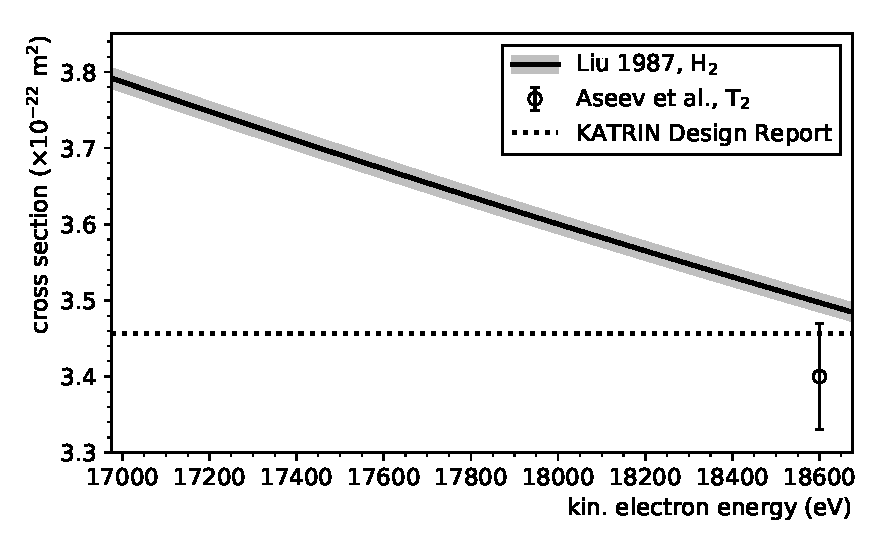
\includegraphics[width=\textwidth]{\currentFigureFolder/crossSecNoZoom.pdf}
	\xcaption{Inelastic cross section for electrons scattering off molecular hydrogen isotopologues}{Inelastic cross section for electrons scattering off molecular hydrogen isotopologues.}{The continuous line shows equation~\eqref{eq:eDepScatCrossSecSourcesCrossSecLiu} for incident electrons with non-relativistic energies with constants from equation~\eqref{eq:eDepScatCrossSecSourcesCrossSecLiuConstantsC1} and~\eqref{eq:eDepScatCrossSecSourcesCrossSecLiuConstantsC2} where the later is assumed to have an uncertainty according to equation~\eqref{eq:eDepScatCrossSecSourcesCrossSecLiuConstantsC2Uncert}. The dashed line shows equation~\eqref{eq:eDepScatCrossSecSourcesCrossSecLiuRelativistic} for incident electrons with relativistic energies. Also, the measurement by~\cite{Aseev2000} at the Troitsk neutrino mass experiment and the value stated in the KATRIN Design Report~\cite{Angrik:2005ep} are depicted. The shown energy interval is chosen according to the \gls{mtd} of the \gls{ft} measurement campaign.}
	\label{fig:eDepScatCrossSecSourcesValues}
\end{figure}

\subsection{Relation to Values of the Inelastic Scattering Cross Section in Former Works}
\label{sec:eDepScatCrossSecSourcesChoice}
As already stated and depicted in figure~\ref{fig:eDepScatCrossSecSourcesValues}, the reference cross section from the KATRIN Design Report does not match the theoretical calculations used in this thesis. Nonetheless, several former works (see subsequent section~\ref{sec:eDepScatCrossSecNuMassInf}) are based on the reference value. Comparability is of importance in the scope of this thesis (as will become apparent in section~\ref{sec:eDepScatCrossSecNuMassInf}). How this issue is addressed is explained in the following.

The cross section value stated in the KATRIN Design Report can be recovered from equation~\eqref{eq:eDepScatCrossSecSourcesCrossSecLiu} if an erroneous energy interpretation is applied. If, instead of equation~\eqref{eq:eDepScatCrossSecSourcesCrossSecNonRelEnergy}, one applies the energy interpretation
\begin{equation}
	\label{eq:eDepScatCrossSecSourcesCrossSecTDREngeryInterpretation}
	T(E) = E
	\comma
\end{equation}
the obtained cross section via equation~\eqref{eq:eDepScatCrossSecSourcesCrossSecLiu} is
\begin{equation}
\label{eq:eDepScatCrossSecSourcesTRDCrossSec}
	\sigma_\mathrm{TDR} 
	\equiv\sigma(E_\mathrm{TDR}=\SI{18565}{eV})
	=\SI{3.4559e-22}{m^2} 
	\approx\SI{3.456e-22}{m^2}
\end{equation}
as stated in the KATRIN Design Report, where the energy $E_\mathrm{TDR}$ is approximately central in the KATRIN design analysis interval (see section~\ref{sec:intSpecModelMTD}). Whether this had been the approach, that had led to the reference cross section in the KATRIN Design Report is not known. 

This work applies the energy interpretation~\eqref{eq:eDepScatCrossSecSourcesCrossSecTDREngeryInterpretation} when comparability to former works, that used the reference cross section from the KATRIN Design Report, is of importance. Otherwise, equation~\eqref{eq:eDepScatCrossSecSourcesCrossSecNonRelEnergy} is used. Corresponding indications are given on a case to case basis. The quantitative difference of these two approaches can be assessed by expanding the $\beta$-factor~\eqref{eq:eDepScatCrossSecSourcesCrossSecBetaFactor} in the ratio $E/m_\elecIndex \approx 18.575/511 \approx 0.036 \ll 1$
\begin{equation}
	\beta^2 \approx 
	2 \frac{E}{m_\elecIndex} - 
	3 \left(\frac{E}{m_\elecIndex}\right)^2
	\fullstop
\end{equation}
The energy interpretation of equation~\eqref{eq:eDepScatCrossSecSourcesCrossSecNonRelEnergy} then becomes
\begin{equation}
	T(E) \approx 0.95 \cdot E
	\comma
\end{equation}
which is a shift in energy and hence, in first order, also in the cross section of about \SI{5}{\percent} compared to the interpretation in equation~\eqref{eq:eDepScatCrossSecSourcesCrossSecTDREngeryInterpretation}. Exact calculations are given in table~\ref{tab:eDepScatCrossSecModelScatProbs}.

\section{An Energy-Dependent Scattering Model using the Poisson Distribution}
\label{sec:eDepScatCrossSecModelPoisson}
The energy-dependence of the cross section enters into the calculation of the scattering probabilities~\eqref{eq:intSpecModelNonAveragedScatProbs}. In the derivation that is given in the previous section~\ref{sec:intSpecModelResponseScattering} the dependence on the starting energy $\Esource$ of electrons is neglected. Instead, an average starting energy and hence an average scattering cross section
\begin{equation}
	\sigma_\mathrm{TDR}(E_\mathrm{TDR})=\SI{3.456e-22}{m^2}
\end{equation}  (energy interpretation as per equation~\ref{eq:eDepScatCrossSecSourcesCrossSecTDREngeryInterpretation}) is assumed. Table~\ref{tab:eDepScatCrossSecModelScatProbs} lists the corresponding scattering probabilities averaged over all starting positions and pitch angles of electrons. Additionally, the results of a Monte Carlo particle tracking simulation by~\cite{Groh2015} and the values using the energy interpretation of equation~\eqref{eq:eDepScatCrossSecSourcesCrossSecNonRelEnergy} are given. How, instead of assuming energy-independent scattering probabilities, the energy-dependence can be modeled is shown in the following.
\begin{table}[t]
	\centering
	\xcaption{Probability for severalfold electron-scattering in the \glsentryshort{wgts} - reviewed}{Probability for severalfold electron-scattering in the \glsentryshort{wgts}.}{The probabilities are averaged over all starting positions and starting pitch angles. Both, the values from a Monte Carlo (MC) particle tracking simulation and the values according to equation~\eqref{eq:intSpecModelAveragedScatProbs} are given. The  cross section was evaluated at an energy of $E_\mathrm{TDR}=\SI{18564.37463}{eV}$ for the two energy interpretations described by equation~\eqref{eq:eDepScatCrossSecSourcesCrossSecTDREngeryInterpretation} and~\eqref{eq:eDepScatCrossSecSourcesCrossSecNonRelEnergy}. Further input parameters to the calculations are a constant gas column density $\rho d = \SI{5e17}{cm^{-2}}$, 
	a \gls{wgts} length of $d=\SI{10.0820}{m}$
	and a maximum acceptance angle of $\thetaMax=\SI{50.7685}{\degree}$. The values are given with the precision needed to reproduce the results in the table below in all digits, which is the precision used in \glsentryshort{ssc}. The energy is chosen such, that $\sigma_\mathrm{TDR}=\SI{3.456000e-22}{m^2}$ is recovered in more than 3 digits as per equation~\eqref{eq:eDepScatCrossSecSourcesTRDCrossSec}.}
	\begin{tabular}{lllr}
		\toprule
		\makecell[tl]{cross section (\SI{e-22}{m^2}) $\rightarrow$} &
		3.456 &
		3.456 &
		3.673 \\
		\hline
		\makecell[tl]{source $\rightarrow$} & 
		\makecell[tl]{MC particle tracking\\ \cite{Groh2015}} & 
		\makecell[tl]{eq.~\eqref{eq:intSpecModelAveragedScatProbs} \\ \cite{Groh2015, Kleesiek2014}} &
		\makecell[tr]{eq.~\eqref{eq:intSpecModelAveragedScatProbs}}
		\\
		\hline
		\makecell[cl]{scattering count $\downarrow$} & 
		& 
	    & \\
		\hline
		\makecell{0} & $0.415 \pm 0.002$ & 0.41334 & 0.39564 \\
		\makecell{1} & $0.292 \pm 0.002$ & 0.29266 & 0.28967 \\
		\makecell{2} & $0.166 \pm 0.001$ & 0.16733 & 0.17298 \\
		\makecell{3} & $0.079 \pm 0.001$ & 0.07913 & 0.08590 \\
		\makecell{4} & $0.031 \pm 0.001$ & 0.03178 & 0.03634 \\
		\bottomrule
	\end{tabular}
	\label{tab:eDepScatCrossSecModelScatProbs}
\end{table}

\begin{figure}[th]
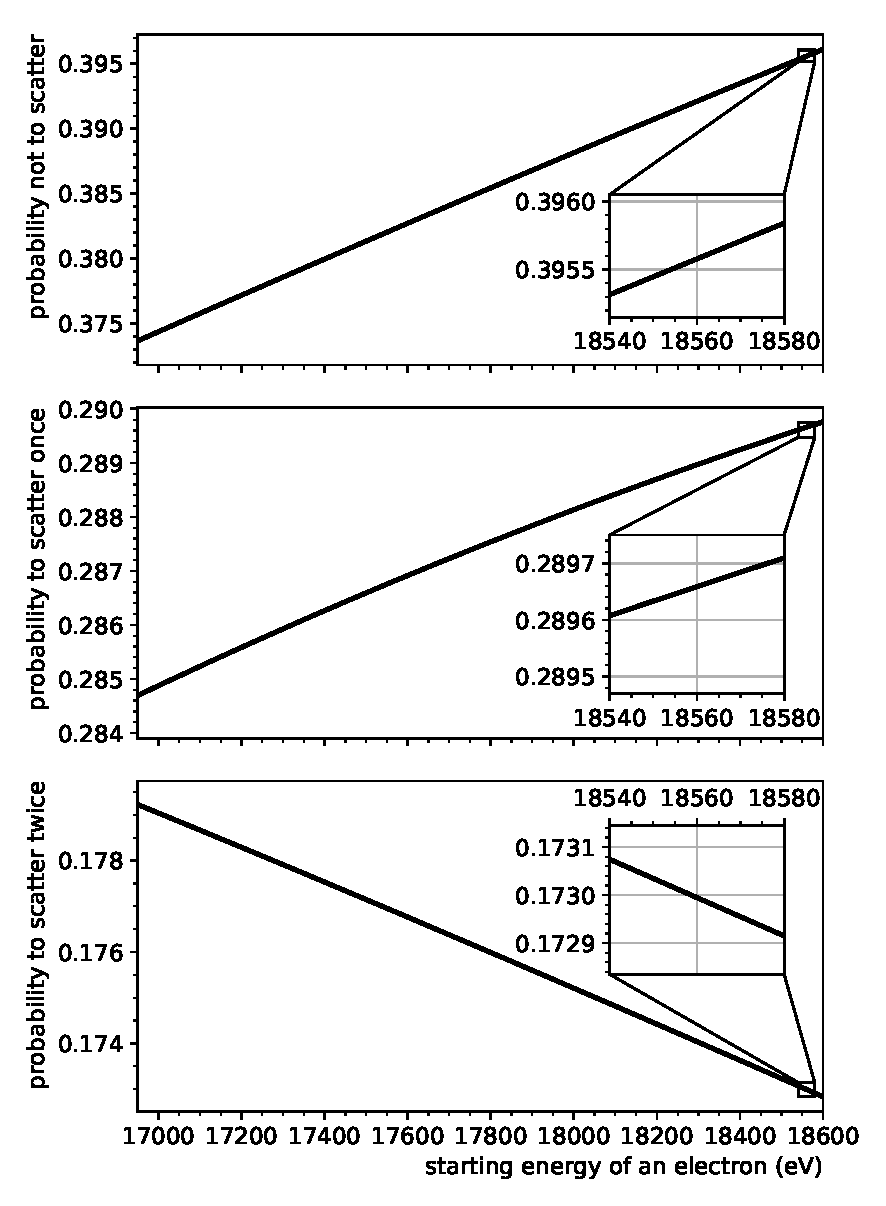
\includegraphics[width=\textwidth]{\currentFigureFolder/scatProbs012Poisson.pdf}
        \xcaption{Probability for severalfold electron-scattering in the \glsentryshort{wgts}}{Probability for severalfold electron-scattering in the \glsentryshort{wgts}.}{From top to bottom, the probability for no, one-fold and two-fold scattering are shown averaged over all starting positions and starting pitch angles of electrons in the \gls{wgts} according to the Poisson Model in equation~\eqref{eq:eDepScatCrossSecModelPoisson}. The shown energy range matches the measurement range of the \gls{ft} measurement campaign and the inset shows an energy span around the endpoint of the tritium $\upbeta$~spectrum.}
        \label{fig:eDepScatCrossSecModel}
\end{figure}

\subsection{The Poisson Model for Electron Scattering}
An expression for the probability of $l$-fold scattering of electrons within the \gls{wgts} is derived in the previous section~\ref{sec:intSpecModelResponseScattering}. The given model is independent of the energy of the electrons. Instead of using a constant cross section, the energy-dependence can be respected. The corresponding formulae from section~\ref{sec:intSpecModelResponseScattering} are repeated below, with the energy-dependence made explicit and by using an energy-dependent cross section as per equation~\eqref{eq:eDepScatCrossSecSourcesCrossSecLiu}
\begin{subequations}
\label{eq:eDepScatCrossSecModelPoisson}
\begin{align}
    \mu(\Esource,\zSource,\thetaSource) =&
    \frac{\sigma(\Esource)}{\cos\thetaSource}
    \int_{\zSource}^{d/2} \rho(z)\d z \label{eq:energydepScatProbsPoissonExpectedScatCount} 
    \comma\\
    P_l(\Esource,\zSource,\thetaSource) =&
    \mathrm{Poisson}(\mu(\Esource,\zSource,\thetaSource),l) \label{eq:eDepScatCrossSecModelPoissonNonAveragedScatProbs} 
    \comma \\
    \bar{P}_l(\Esource) =&
    \frac{1}{d \cdot (1-\cos(\thetaMax))} 
      \int_{-d/2}^{d/2}  
          \int_{0}^{\theta_{max}} 
            \sin(\thetaSource)
            \mathrm{Poisson}(\mu(\Esource,\zSource,\thetaSource),l)
          \d\thetaSource
      \d\zSource
      \label{eq:eDepScatCrossSecModelPoissonAveragedScatProbs}
    \fullstop
\end{align}
\end{subequations}
As a reminder, $\bar{P}_l(\Esource)$ in equation~\eqref{eq:eDepScatCrossSecModelPoissonAveragedScatProbs} denotes the probability for $l$-fold scattering of an electron with a starting kinetic energy $\Esource$ averaged over all starting positions and pitch angles in the \gls{wgts}. In the following, this model is denoted ``Poisson model''. 

\subsection{Properties of the Poisson Model for Electron Scattering}
\label{sec:eDepScatCrossSecModelPoissonProperties}
Figure~\ref{fig:eDepScatCrossSecModel} shows the Poisson model as per equation~\eqref{eq:eDepScatCrossSecModelPoisson}. Table \ref{tab:eDepScatCrossSecModelScatProbs} lists the scattering probabilities for an energy-independent Poisson model (see section~\ref{sec:intSpecModelResponseScattering}) and a reference cross section $\sigma(E\approx\SI{18564}{eV})=\SI{3.673e-22}{m}$. The energy-dependent Poisson model recovers the energy-independent model exactly at the corresponding energy as expected.

\paragraph{Trend of the Energy-Dependence}
\begin{figure}[th]
	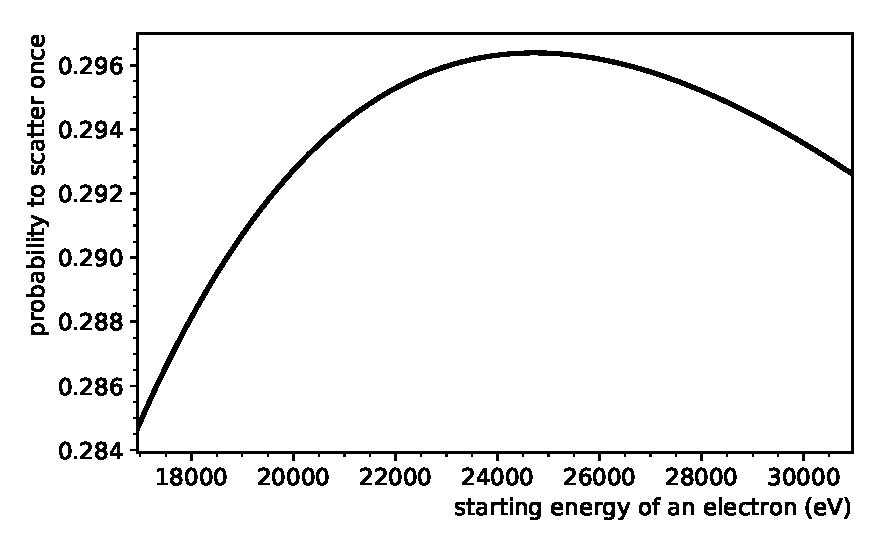
\includegraphics[width=\textwidth]{\currentFigureFolder/scatProbs1Poisson_extendedEnergyRange.pdf}
	\xcaption{Probability for one-fold electron-scattering in the \glsentryshort{wgts} in an extended energy range}{Probability for one-fold electron-scattering in the \glsentryshort{wgts} in an extended energy range.}{The graph shows the probability of one-fold scattering according to equation~\eqref{eq:eDepScatCrossSecModelPoissonAveragedScatProbs}. It emphasizes the change of sign in the derivative at approximately \SI{24.7}{keV}.}
	\label{fig:eDepScatCrossSecModelPoissonP1ExtendedEnergyRange}
\end{figure}
As depicted in figure~\ref{fig:eDepScatCrossSecModel}, for an increasing starting energy of electrons within the \gls{wgts}, the probability for no and one-fold scattering also increases, while the probability for two-fold scattering decreases. This paragraph aims to give an intuitive argument for this change of sign in the derivative $\d \bar{P}_l(\Esource) / \d \Esource$ in the transition from $l=1$ to $l=2$. The Poisson model $\bar{P}_l(\Esource)$ is a probability density in $l$ for a fixed $\Esource$ (see appendix~\ref{sec:appendixEDepScatCrossSecPoissonModelProbDensityProof} for a proof). Hence, the expected scattering count for an energy within the range of starting energies $\Esource \in [\SI{17}{keV}, \SI{18.6}{keV}]$, that is depicted in figure~\ref{fig:eDepScatCrossSecModel}, can be calculated (numerically)
\begin{equation}
\label{eq:eDepScatCrossSecModelPoissonExpectedScatCount}
\begin{split}	
	\bar{l}(\SI{17.0}{keV}) &= 
	\sum_{l}^{\infty} \bar{P}_l(\SI{17.0}{keV}) \cdot l \approx 1.23 \\	
	\bar{l}(\SI{18.6}{keV}) &= 
	\sum_{l}^{\infty} \bar{P}_l(\SI{18.6}{keV}) \cdot l \approx 1.14
	\fullstop
\end{split}
\end{equation} 
In other words, electrons with a starting energy between \SI{17}{keV} and \SI{18.6}{keV} are expected to scatter between 1 and 2 times on their way through the \gls{wgts} (averaged over all starting positions and pitch angles). Then, the illustrative line of argument is the following: 
\begin{align*}
	&\text{ the starting energy $\Esource$ increases} \\ \Rightarrow
	&\text{ the scattering cross section decreases (see figure~\ref{fig:eDepScatCrossSecSourcesValues})} \\ \Rightarrow
	&\text{ scattering becomes less likely} \\ \Rightarrow
	&\text{ $\bar{l}$ decreases and moves closer to 1 and away from 2} \\ \Rightarrow
	&\text{ the probability for no and one-fold scattering increases,} \\
	&\text{ while the probability for more than one scattering decreases}
	\fullstop
\end{align*} 
This is in accordance with the trend of the energy-dependence depicted in figure~\ref{fig:eDepScatCrossSecModel}. Also, if this reasoning is correct, the sign of $\d \bar{P}_1(\Esource) / \d \Esource$ for one-fold scattering should change for sufficiently high energies and the probability to scatter once should decrease. This is indeed the case as depicted in figure~\ref{fig:eDepScatCrossSecModelPoissonP1ExtendedEnergyRange}. The decrease starts at an energy of roughly \SI{24.7}{keV}. This might for example be of relevance for the measurement of Krypton conversion lines in calibration measurements because the corresponding electron energies are above \SI{30}{keV}~\cite{venos2018}.


\paragraph{Limit of the Poisson Model for Electron Scattering}
The Poisson model is exact for the probability of no scattering $\bar{P}_0(\Esource)$, but it does not hold for one or more scatterings because an electron loses energy when scattering. The scattering cross section increases with decreasing energy (see figure~\ref{fig:eDepScatCrossSecSourcesValues}) and the electron becomes more likely to scatter again. In other words, the probabilities of individual scattering processes are no longer independent when respecting the dependence on the electron energy. This violates one of the preconditions to model the scattering probabilities via a Poisson distribution. Another model beyond the description via a Poisson distribution is suggested in the subsequent section~\ref{sec:eDepScatCrossSecModelExtended}. However, at the current stage, this extended model poses computational difficulties as is discussed in section~\ref{sec:eDepScatCrossSecExtendedModelNumEval}. The aim of this thesis is the assessment of energy-dependent effects. This can already be achieved with the Poisson model as shown in the previous paragraphs. Therefore, the Poisson model was further used to address the energy-dependent effects in the scope of neutrino mass inference.
\FloatBarrier

\paragraph{Implementation and Performance}
Within the scope of this thesis, the energy-dependent Poisson model of equation~\eqref{eq:eDepScatCrossSecModelPoisson} was implemented into the \gls{ssc} software framework. The energy-dependence of the scattering cross section may not be negligible in neutrino mass inference as is explained in the subsequent section~\ref{sec:eDepScatCrossSecNuMassInf}. For that reason, the impact on the fitting run time by using an energy-dependent cross section was probed. Depending on the \gls{mtd}, a fit might become slower by a factor of 40 to 120. This is due to the fact, that, when integrating over the energy loss in the response function in equation~\eqref{eq:intSpecModelResponse}, the scattering probabilities have to be recomputed in every step of the numerical integration. It might be beneficial to investigate whether the evaluation can be speed up in the future. For example, it might be sufficient to only compute the energy-dependent scattering probabilities for a limited set of energies and interpolate them in-between those energies.

\section{Effects of Systematic Cross-Section Offsets in Neutrino Mass Inference}
\label{sec:eDepScatCrossSecNuMassInf}
It was investigated, how much the squared neutrino mass that is inferred from a KATRIN measurement would be shifted if the energy-dependence of the scattering cross section is neglected in the corresponding fitting procedure. The comparability to former results is of importance within this section. For that reason, the energy interpretation of equation~\eqref{eq:eDepScatCrossSecSourcesCrossSecTDREngeryInterpretation} is used, which yields a cross section of $\sigma_\mathrm{TDR}=\SI{3.456e-22}{m^2}$ at an energy of \SI{18565}{eV} within the KATRIN design analysis interval. There are several previous works that studied similar effects~\cite{Antoni2015,Groh2015,SeitzM2019,Kuckert2016,Kuckert2018}. In section~\ref{sec:eDepScatCrossSecNuMassInfGroh}, the results from~\cite{Groh2015} are reviewed representatively for the mentioned works because they might intuitively contradict the results obtained in this thesis. In section~\ref{sec:eDepScatCrossSecNuMassInfThisWork}, the results of this thesis are listed. And in section~\ref{sec:eDepScatCrossSecNuMassInfRelateGrohAndFormerWork}, an argument is given, why both sets of results are assumed to be in accordance.

\subsection{Neutrino Mass Shifts for an Energy-Independent Cross-Section Offset from Former Works}
\label{sec:eDepScatCrossSecNuMassInfGroh}
In~\cite{Groh2015}, it was investigated how much a constant offset of the cross section would shift the inferred squared neutrino mass if the offset were neglected in the analysis. A rule of thumb for the shift in dependence on the relative offset of the cross section $\Delta\sigma/\sigma_\mathrm{TDR}$ is given~\cite{Groh2015}
\begin{equation}
	\label{eq:eDepScatCrossSecNuMassInfShiftRuleOfThumb}
	\frac{\Delta\nuMass^2(\Delta\sigma)}{\SI{e-3}{eV^2}} =
	-0.45
	-1204\cdot
	\frac{
		\Delta\sigma
	}{
		\sigma_\mathrm{TDR}
	}
	\qquad \text{ with } \quad 
	\sigma_\mathrm{TDR} = \SI{3.456e-22}{m^{-2}}
	\fullstop
\end{equation}
This rule of thumb was deduced via a linear approximation of several neutrino mass shifts in dependence of the relative cross section offset. Although, it can only be used for rough estimations, it serves well for the discussion in the following sections. Using the energy interpretation of the KATRIN Design Report (eq.~\ref{eq:eDepScatCrossSecSourcesCrossSecTDREngeryInterpretation}) and the numerical inversion of the cross section formula (eq.~\ref{eq:eDepScatCrossSecSourcesCrossSecLiu}), in the KATRIN design analysis interval of \SI{30}{eV}, the relative offset of the cross section caused by the energy-dependence is
\begin{equation}
	\label{eq:eDepScatCrossSecNuMassInfRelativeCrossSecOffset}
	\left|
	\frac{
		\Delta\sigma
	}{
		\sigma_\mathrm{TDR}
	}
	\right| < \SI{0.1}{\percent}
	\fullstop
\end{equation}
Thus, the rule of thumb~\eqref{eq:eDepScatCrossSecNuMassInfShiftRuleOfThumb} yields
\begin{equation}
	\label{eq:eDepScatCrossSecNuMassInfShiftEstimate}
	\left|
		\Delta\nuMass^2(\Delta\sigma)
	\right| < \SI{2e-3}{eV^2} 
\end{equation}
within the KATRIN design analysis interval of \SI{30}{eV}.

\subsection{Neutrino Mass Shifts for an Energy-Dependent Cross-Section Offset}
\label{sec:eDepScatCrossSecNuMassInfThisWork}
\begin{figure}[t]
	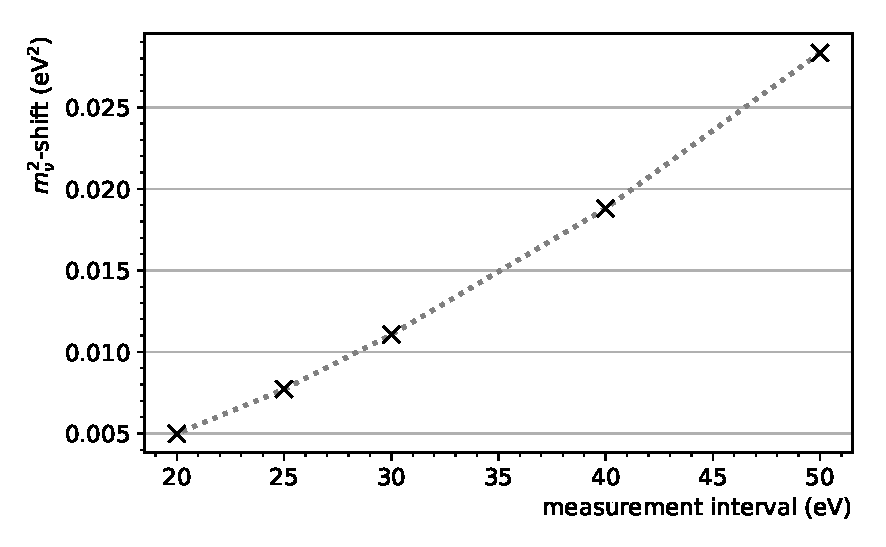
\includegraphics[width=\textwidth]{\currentFigureFolder/nuMassShiftForEDepCrossSec.pdf}
	\xcaption{Shift of an inferred squared neutrino mass induced by a neglected energy-dependence of the inelastic scattering cross section}{Shift of an inferred squared neutrino mass induced by a neglected energy-dependence of the inelastic scattering cross section.}{The neutrino mass was inferred from data that was simulated using an energy-dependent inelastic scattering cross section as per equation~\eqref{eq:eDepScatCrossSecSourcesCrossSecLiu} (with an energy interpretation according to equation~\eqref{eq:eDepScatCrossSecSourcesCrossSecTDREngeryInterpretation} for compatibility with the KATRIN Design Report) and using a nominal four-parameter fit model that assumes a constant cross section of $\sigma_\mathrm{TDR}=\SI{3.456e-22}{m^2}$. The procedure was repeated for five different measurement intervals (respectively \gls{mtd}s) $[E_0-\alpha, E_0+\SI{5}{eV}]$ based on the KATRIN Design Report where $\alpha$ is denoted on the abscissa and $E_0=\SI{18575}{eV}$ is the endpoint of the $\upbeta$ spectrum. The \gls{mtd}s are listed in appendix~\ref{sec:appendixEDepScatCrossSecMTDs}. The markers show the results for the obtained shift of the squared neutrino mass and the dotted line is an interpolation in-between. The study was done once with a free fit parameter for the endpoint and once having it fixed to the simulation truth in order to show the influence on the sign of the shift of the squared neutrino mass (for details refer to the the main text).}
	\label{fig:eDepScatCrossSecNuMassInfShifts}
\end{figure}
In the scope of this thesis, an energy-dependent offset of the cross section was investigated (in contrast to a constant one in~\cite{Groh2015}). A KATRIN neutrino mass measurement for a neutrino mass of \SI{0}{eV} was simulated using an energy-dependent cross section\footnote{In all studies presented in this chapter, the simulated electron detector counts were substituted by their expectation values as opposed to fluctuated according to Poissonian statistics. In other words, no ensemble testing was done. For more details on such an Asimov data set and why it can reasonably be assumed to be representative for an ensemble, see section~\ref{sec:katrinElossStatisticsAsimov}.}. A model that uses a constant cross section was fitted to the simulated spectrum. This procedure was repeated for five different \gls{mtd}s of different measurement intervals. Figure~\ref{fig:eDepScatCrossSecNuMassInfShifts} shows the results. For the KATRIN design measurement interval of~\SI{30}{eV}, the difference from \SI{0}{eV}, respectively the shift of the squared neutrino mass, is
\begin{equation}
	\label{eq:eDepScatCrossSecNuMassInfShiftByThisThesis}
	\Delta\nuMass^2 = \SI{1.09e-2}{eV^2}
	\fullstop
\end{equation}
First, it should be noted that this value is greater by a factor of $\sim5$ than the one stated above in equation~\eqref{eq:eDepScatCrossSecNuMassInfShiftEstimate}, that was estimated using the results from~\cite{Groh2015}. This issue is addressed in the subsequent section~\ref{sec:eDepScatCrossSecNuMassInfRelateGrohAndFormerWork}. Further aspects are discussed in the following paragraph:

\paragraph{Sign of the Shift of the Squared Neutrino Mass}
Using an energy-dependent cross section in the simulation and neglecting it in neutrino mass inference yields a higher $\upbeta$ electron count in the endpoint region than expected (see figure~\ref{fig:eDepScatCrossSecNuMassInfIntegralRate}) because the cross section decreases with higher energies and electrons of higher energies are less probable to scatter. On one hand, a higher $\upbeta$ electron count for energies in the endpoint region of the $\upbeta$ spectrum can be caused by a lower squared neutrino mass. On the other hand, a higher $\upbeta$ electron count can also be caused by a higher endpoint of the $\upbeta$ spectrum. These two effects counterbalance each other, which makes it difficult to make an intuitive, qualitative statement about the sign of the shift of the squared neutrino mass. As shown in equation~\eqref{eq:eDepScatCrossSecNuMassInfShiftByThisThesis}, the shift of the squared neutrino mass is positive. However, if the above reasoning is correct, then one should obtain a flip in the sign of the shift if the endpoint is not taken as a free fit parameter, but fixed to the simulation truth. Figure~\ref{fig:eDepScatCrossSecNuMassInfShifts} shows that this is indeed the case.

\paragraph{Significance for the KATRIN Experiment}
The shift of the squared neutrino mass in equation~\eqref{eq:eDepScatCrossSecNuMassInfShiftByThisThesis} takes a sizable fraction of the systematic budget of \SI{1.7e-2}{eV^2} (see eq.~\ref{eq:statMethodsSensitivtyFromEnsembleTDRSysBudget}) of the KATRIN experiment, but is still smaller. Hence, whether the effect of the energy-dependence of the scattering cross section can be neglected depends on the contribution of other systematic effects and can not yet fully be assessed (see for example~\cite{SeitzM2019} for a comprehensive list of systematic effects with regard to the KATRIN experiment).

It should be mentioned that KATRIN's design allows to measure the product of the gas column density and the inelastic scattering cross section $\rho d \cdot \sigma(E)$ for a fixed electron energy~$E$ using the electron gun. In order to respect the energy dependence of the cross section, it is necessary to incorporate a corresponding model, such as the formula for the energy-dependent cross section (eq.~\ref{eq:eDepScatCrossSecSourcesCrossSecLiu}). This might enable the measurement of the two constants $C_1$ and $C_2$ in said formula. Therefore, $\rho d \cdot \sigma(E)$ has to be measured for multiple energies $E$. Such measurements were already conducted at the KATRIN experiment. However, results that respect the energy-dependence of the scattering cross section are not yet available at the time of writing this thesis.

\subsection{Relation of the Shifts for an Energy-Dependent and -Independent Cross-Section Offset}
\label{sec:eDepScatCrossSecNuMassInfRelateGrohAndFormerWork}
In the scope of this thesis, the shift of an inferred neutrino mass that is introduced by neglecting the energy-dependence of the cross section was investigated. Former works investigated the shift when neglecting a constant offset of the cross section. The shift obtained in this thesis in equation~\eqref{eq:eDepScatCrossSecNuMassInfShiftByThisThesis} is $\sim5$ times larger than the one obtained by the former study in~\cite{Groh2015} under equation~\eqref{eq:eDepScatCrossSecNuMassInfShiftEstimate}, although the energy-dependent offset of the cross section is never greater than the constant offset investigated by~\cite{Groh2015}. This might be contra intuitive, but a possible explanation is the following: The fit parameter for the signal amplitude $\sigAmp$ in a nominal KATRIN fit (see section~\ref{sec:statMethodsStandardFit}) can partly compensate for a constant offset of the cross section. However, it cannot compensate for an energy-dependent one equally well. This is demonstrated below:

The study from~\cite{Groh2015} was reproduced with a free fit parameter for the signal amplitude $\sigAmp$. The reproduced study was in accordance with the values in~\cite{Groh2015}. Then, $\sigAmp=1$ was fixed. The results are shown in figure~\ref{fig:eDepScatCrossSecNuMassInfShiftsForConstCrossSec}. A relative cross section offset of $
\left|
	\Delta\sigma/\sigma_\mathrm{TDR}
\right| \approx \SI{0.1}{\percent}
$ (see equation~\ref{eq:eDepScatCrossSecNuMassInfRelativeCrossSecOffset}) yields a shift of the squared neutrino mass, that is larger by almost an order of magnitude with a fixed $\sigAmp$ as opposed to leaving $\sigAmp$ as a free parameter. The shift is then greater than the one obtained in the the study presented in the previous section~\ref{sec:eDepScatCrossSecNuMassInfThisWork} that uses an energy-dependent cross section in the \SI{30}{eV} measurement interval. This verifies, that the fit parameter for the signal amplitude $\sigAmp$ can partly compensate for a constant offset of the cross section. 

Additionally, the following plausibility argument can be given: Figure~\ref{fig:eDepScatCrossSecNuMassInfIntegralRate} shows the simulated integral rate for different cross section models normalized to the integral rate obtained by using the model with a constant cross section $\sigma_\mathrm{TDR}$ from the KATRIN Design Report. The integral rates that are based on a model with a constant, energy-independent cross section differ from each other by almost a constant factor (variations $<2\times10^{-4}$). This implies, when one of these models is used in a simulation of a KATRIN measurement and another model is used in a corresponding fit for neutrino mass inference, their difference can be compensated by the fit parameter for the signal amplitude $\sigAmp$. However, the model that uses an energy-dependent cross section does not differs from the one with the constant cross section $\sigma_\mathrm{TDR}$ by a factor, that varies over the energy range. Such a difference can not be compensated by the fit parameter for the signal amplitude $\sigAmp$.

\begin{figure}[t]
	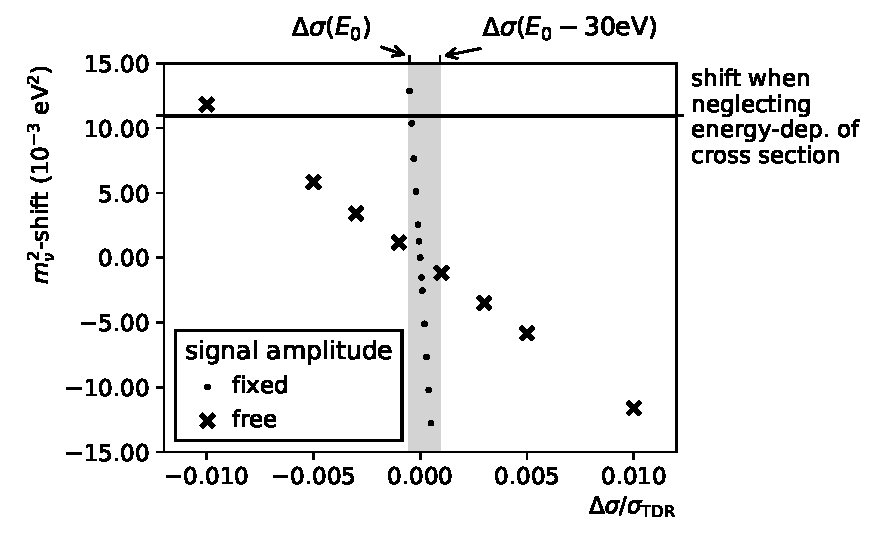
\includegraphics[width=\textwidth]{\currentFigureFolder/nuMassShiftForConstCrossSec.pdf}
	\xcaption{Shift of an inferred squared neutrino mass induced by a neglected constant offset of the inelastic scattering cross section}{Shift of an inferred squared neutrino mass induced by a neglected constant offset of the inelastic scattering cross section.}{The neutrino mass was inferred from data that was simulated using different constant inelastic scattering cross sections. The abscissa shows the offset of the used inelastic scattering cross section relative to $\sigma_\mathrm{TDR}=\SI{3.456e-22}{m^2}$, which was used in the assumed fit model. In an energy-dependent scenario, a cross section corresponds an energy of incident electrons as per equation~\eqref{eq:eDepScatCrossSecSourcesCrossSecLiu}. The cross section range, that corresponds the design KATRIN analysis energy interval of \SI{30}{eV} is depicted as a gray band (energy interpretation as per eq.~\ref{eq:eDepScatCrossSecSourcesCrossSecTDREngeryInterpretation}). The analysis was done twice: once with a free parameter for the signal amplitude, which reproduced the results given in~\cite{Groh2015}~(figure 6.31 on page 221); the second analysis had this parameter fixed. The shift  obtained for $\Delta\sigma/\sigma_\mathrm{TDR}\approx\SI{-0.1}{\percent}$ and a fixed signal amplitude is greater than the shift obtained when neglecting the energy-dependence of the cross section within the \SI{30}{eV} measurement interval (depicted by the horizontal line).}
	\label{fig:eDepScatCrossSecNuMassInfShiftsForConstCrossSec}
\end{figure}


\begin{figure}[t]
	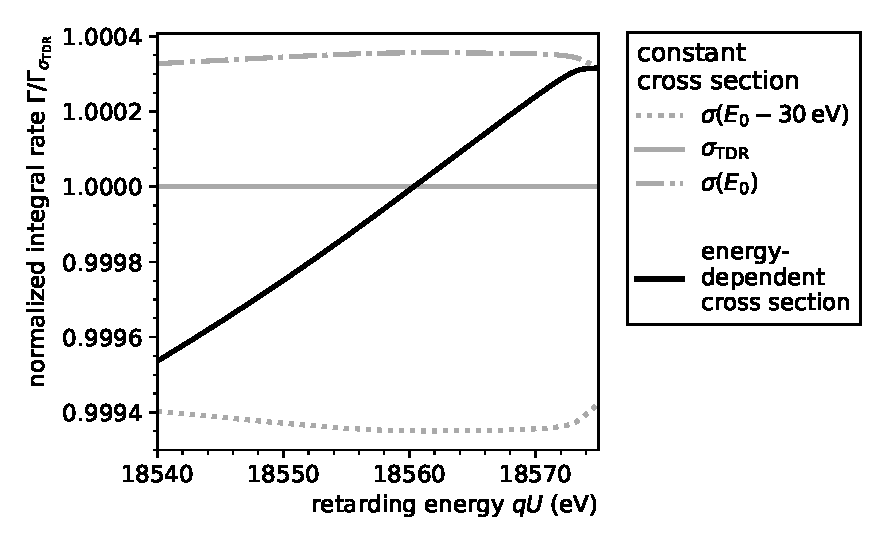
\includegraphics[width=\textwidth]{\currentFigureFolder/normedIntegralRate.pdf}
	\xcaption{Simulated integral $\upbeta$-electron rate using different models of the cross section for inelastic electron-scattering}{Simulated integral $\boldsymbol{\upbeta}$-electron rate using different models of the cross section for inelastic electron-scattering.}{The abscissa shows the energy range of the design KATRIN analysis interval of \SI{30}{eV}. The lines show the integral rate of $\upbeta$~electrons for different models for the inelastic scattering cross section normalized to the model that uses the constant cross section $\sigma_\mathrm{TDR}=\SI{3.456e-22}{m^2}$. The gray lines use a model with a constant cross section. The cross section values can be identified with electron energies as per equation~\eqref{eq:eDepScatCrossSecSourcesCrossSecLiu} and the energy interpretation of equation~\eqref{eq:eDepScatCrossSecSourcesCrossSecTDREngeryInterpretation} with $\sigma(E_0-\SI{30}{eV}=\SI{18545}{eV})=\SI{3.459e-22}{m^2}$ and $\sigma(E_0=\SI{18575}{eV})=\SI{3.454e-22}{m^2}$. The black line shows the simulated integral rate for an energy-dependent cross section. This graph emphasizes that the integral rates for models using a constant cross section differ by an almost constant factor, whereas the rate using an energy-dependent cross section differs from the others by a varying factor.}
	\label{fig:eDepScatCrossSecNuMassInfIntegralRate}
\end{figure}
\FloatBarrier

\section{An Energy-Dependent Scattering Model beyond Using the Poisson Distribution}
\label{sec:eDepScatCrossSecModelExtended}
In the previous section~\ref{sec:eDepScatCrossSecModelPoisson} the scattering probabilities are modeled using a Poisson distribution. This introduces an error for the following reason: A scattering electron loses energy. The scattering cross section increases with decreasing energy (see figure~\ref{fig:eDepScatCrossSecSourcesValues}) and the electron becomes more likely to scatter again. In other words, the probabilities of individual scattering processes are not independent when respecting the dependence on the electron energy. This violates one of the preconditions to model the scattering probabilities via a Poisson distribution. 

This section aims to quantify the error that is introduced by the approximate modeling via a Poisson distribution. Another model is suggested\footnote{The idea was inspired by a model in~\cite{Groh2015} that incorporates changes of the electron pitch angle due to scattering.} in section~\ref{sec:eDepScatCrossSecExtendedModelFormalism} that partly accounts for the energy loss of electrons in the formalism of the scattering probabilities. The suggested model was evaluated numerically as it includes one limit and two integrals that could not yet be solved analytically. The numerical accuracy had to be good enough to decide whether it differs significantly from the Poisson model or not. At the same time, a balance between the numerical accuracy and the evaluation run time had to be found. This matter is described in detail in section~\ref{sec:eDepScatCrossSecExtendedModelNumEval}. The results of the numerical evaluation are discussed in section~\ref{sec:eDepScatCrossSecExtendedModelDiscussion}.

\subsection{Mathematical Formalism of the Extended Model for Electron Scattering}
\label{sec:eDepScatCrossSecExtendedModelFormalism}
In the following, a model for the probability of electron-scattering in the \gls{wgts} that depends on the electron energy is derived. The difficulty lies in the fact, that an electron that scatters loses energy and hence its probability to scatter a second time is different from the first time. The presented model assumes the same fixed energy loss $\epsilon$ for each scattering in contrast to a realistic distribution as given by the energy loss function (see figure~\ref{fig:intSpecModelAseevEloss}). This was sufficient to show a difference in the Poisson model and the model suggested below. However, a more accurate description would incorporate the full energy loss function. This may be the subject of a future study. 

The aim of this section is the derivation of an expression $\bar{P}^{\star}_l(\Esource)$ that denotes the probability of $l$-fold scattering for an electron with a starting energy $\Esource$ averaged over all starting positions and pitch angles assuming a fixed energy loss $\epsilon$ per scattering.

The expected amount of scatterings for an electron when traveling through the whole \gls{wgts} volume of length $d$ filled with a gas of constant density $\rho$ is (see equation~\ref{eq:intSpecModelExpectedScatteringCount})
\begin{equation}
\label{eq:eDepScatCrossSecExtendedModelFormalismExpectedScatCount}
\mu(E,\thetaSource) =
\frac{\sigma(E)\rho d}{\cos\thetaSource},
\end{equation}
where $E$ denotes the electron's kinetic energy; $\thetaSource$ the starting pitch angle; and $\sigma(E)$ the energy dependent scattering cross section. It should be noted that the energy $E$ is denoted without and index S here, because, in the following, this formula is reused for different electron energies, not only the starting energy of an electron.

In the following, the volume of the \gls{wgts} is thought of being divided into $N$ slices of equal width $w=L/N$ (and later the limit $N\rightarrow\infty$ is applied). $N$ is chosen sufficiently large that the probability for an electron to scatter twice within one slice is essentially zero. Then, for large $N$, the probability to scatter within one slice is $\mu(E,\thetaSource)/N$. The probability not to scatter within $n \leq N$ slices is
\begin{equation}
p_0(E,\thetaSource,n) =
\left(
1-\frac{\mu(E,\thetaSource)}{N}
\right)^n
\fullstop
\end{equation}
Let ``Poisson($\mu$,$l$)'' denote the Poisson distribution with expectation value $\mu$ and evaluated at $l$. Using the well known limit for the Euler constant, one obtains for $n=N$ and $N\rightarrow\infty$ that $p_0$ is a Poisson distribution with the expectation value $\mu$ from equation~\eqref{eq:eDepScatCrossSecExtendedModelFormalismExpectedScatCount} and evaluated at $l=0$ 
\begin{align}
\label{eq:eDepScatCrossSecExtendedModelFormalismRecoveryOfPoisson}
\lim_{N\rightarrow\infty} 
p_0(E,\thetaSource,N) =
\lim_{N\rightarrow\infty} 
\left(
1-\frac{\mu(E,\thetaSource)}{N}
\right)^N =
\mathrm{e}^{-\mu(E,\thetaSource)} = 
\mathrm{Poisson}(\mu(E,\thetaSource), 0)
\fullstop
\end{align}
In other words, for no scattering, the Poisson model for the scattering probabilities as described in section~\ref{sec:eDepScatCrossSecModelPoisson} is recovered.

Assuming a constant energy loss $\epsilon$ per scattering, the probability to scatter $l>0$ times within $n<N$ slices can be expressed recursively
\begin{equation}
\label{eq:eDepScatCrossSecExtendedModelFormalismCore}
p_l(E,\thetaSource,n) =
\underbrace{
	\sum_{k=l}^{n}
}_{(4)}
\underbrace{
	p_{l-1}(E,\thetaSource,k-1)
	\vphantom{\sum_{k=l}^{n}}
}_{(1)}
\underbrace{
	\left(
	1-p_0(E-(l-1)\epsilon,\thetaSource,1)
	\right)
	\vphantom{\sum_{k=l}^{n}}
}_{(2)}
\underbrace{
	p_0(E-l\epsilon,\thetaSource,n-k)
	\vphantom{\sum_{k=l}^{n}}
}_{(3)}
\fullstop
\end{equation}
The idea behind this expression is the following: One imagines an electron with an energy $E$ that travels through $n$ \gls{wgts} slices, scatters $l$ times in total and the last time in the $k$th slice. Hence, it must have scattered $l-1$ times in the $k-1$ slices before the $k$th slice and must not scatter in the $n-k$ slices to follow. In that regard, the above expressions have the following meaning:
\begin{enumerate}[(1)]
	\item Probability to scatter $l-1$ times within $k-1$ slices with a kinetic energy of $E$.
	\item Probability to scatter once within the $k$th slice with a kinetic energy of $E-(l-1)\epsilon$.
	\item Probability not to scatter within the remaining $n-k$ slices with a kinetic energy of $E-l\epsilon$.
	\item Sum over all slices $k$ where the electron could scatter the last time. The sum starts at $l$ (as opposed to 1) because the probability to scatter $l-1$ times within less than $k=l-1$ slices (term (1)) is 0 due to the made assumption, that in the limit of a large amount of slices $N$ an electron does not scatter twice within one slice.
\end{enumerate}
The probability to scatter $l$ times can be averaged over all starting positions of electrons respectively starting slices. In this regard, $\nSource$ denotes the amount of slices an electron has to pass through depending on its starting slice (including its starting slice). Then the average is
\begin{equation}
\label{eq:eDepScatCrossSecExtendedModelFormalismZAverage}
\bar{p}_l(E,\thetaSource) = 
\frac{1}{N}
\sum_{\nSource=1}^{N} p_l(E,\thetaSource,\nSource) \approx
\frac{1}{d}
\int_{0}^{d}
p_l(E,\thetaSource,
\left\lceil N \frac{\zSource}{d}\right\rceil
)
\d \zSource
\fullstop
\end{equation}
Here, the averaging sum is approximated by an integral as this helps cutting down on run time in a numerical evaluation. This is due to the fact, that in a numerical evaluation a large number $N$ ($\sim10^5$) of slices has to be chosen and the sum would have many terms. However, a numerical integration can achieve an accurate result with a smaller set of supporting points (see subsequent section~\ref{sec:eDepScatCrossSecExtendedModelNumEval}). 

Then, the limit $N\rightarrow\infty$ can be applied
\begin{equation}
P^{\star}_l(\Esource,\thetaSource) = 
\lim_{N\rightarrow\infty} \bar{p}_l(\Esource,\thetaSource)
\fullstop
\label{eq:eDepScatCrossSecExtendedModelFormalismPitchAngleDepScatProbs}
\end{equation}
$P^{\star}_l(\Esource,\thetaSource)$ denotes the probability for an electron to scatter $l$ times when traveling through the whole \gls{wgts} with a starting energy $\Esource$ and pitch angle $\thetaSource$ averaged over all starting positions. Finally, this expression can be averaged over all starting pitch angles in order to obtain the energy dependent scattering probabilities
\begin{equation}
\bar{P}^{\star}_l(\Esource) = 
\frac{1}{1-\cos\thetaMax}
\int_0^{\thetaMax}
\sin \thetaSource
P^{\star}_l(\Esource,\thetaSource) 
\d \thetaSource
\fullstop
\label{eq:eDepScatCrossSecExtendedModelFormalismAveragedDepScatProbs}
\end{equation}
$\bar{P}^{\star}_l(\Esource)$ denotes the probability for $l$-fold scattering of an electron with a starting energy $\Esource$ averaged over all starting positions and pitch angles assuming a fixed energy loss $\epsilon$ per scattering. In the following, this model is called the ``extended model''.

\subsection{Numerical Accuracy and Cross-Check of the Extended Model for Electron Scattering}
\label{sec:eDepScatCrossSecExtendedModelNumEval}
\begin{figure}[t]
	\centering
	\includegraphics{chapter/energyDependentCrossSec/fig/scatProb1_numericalAccuracy.pdf}
	\xcaption{Accuracy of the numerical evaluation of the extended model of the probability for electron-scattering in the \glsentryshort{wgts}}{Accuracy of the numerical evaluation of the extended model of the probability for electron-scattering in the \glsentryshort{wgts}.}{The extended model is given by equation~\eqref{eq:eDepScatCrossSecExtendedModelFormalismAveragedDepScatProbs} and the Poisson model is given by equation~\eqref{eq:eDepScatCrossSecModelPoisson}. For both models, the energy of the incident electrons was taken such that the Poisson model yields the values already given in table~\ref{tab:eDepScatCrossSecModelScatProbs}. The left column shows the dependence on the number $N$ of slices of the \gls{wgts}. The right column shows the dependence on the order of Gaussian quadrature that was used to evaluate the two integrals in the extended model. The Poisson model is independent of these features and can be evaluated exactly (limited by machine number precision). In the left column, the order of Gaussian quadrature was fixed to 5 and in the right column, the number of slices was fixed to $5\times10^{5}$. The upper row shows the numerical evaluation of the extended model for no energy loss per scattering (markers). Its exact solution is given by the Poisson model (line). The lower row shows the extended model for an energy loss of \SI{12.6}{eV} per scattering. The upper row shows that the numerical evaluation of the extended model is within a distance of less than $3\times10^{-6}$ of its exact solution and the lower row shows convergence on the $10^{-5}$ level. These results make it plausible to assume a numerical accuracy on the $10^{-5}$ level or better for the shown configurations of the numerical evaluation of the extended model.}
	\label{fig:eDepScatCrossSecExtendedModelNumEval}
\end{figure}
For the evaluation of the energy-dependent scattering probabilities according to the extended model in equation~\eqref{eq:eDepScatCrossSecExtendedModelFormalismAveragedDepScatProbs} the fixed energy loss $\epsilon=\SI{12.6}{eV}$ per scattering was chosen as it is the most probable energy loss for electrons traveling through tritium gas (see figure~\ref{fig:intSpecModelAseevEloss}). The mean value would also have been a possible choice. But the energy loss function as depicted in figure~\ref{fig:intSpecModelAseevEloss} is not normalized to $[0, \infty)$, which poses the problem of finding a suitable energy interval, with respect to which the mean value is calculated. In other words, at the current stage, a certain arbitrarity concerning the energy loss per scattering could not be avoided. As already mentioned, a future study might consider a more comprehensive incorporation of the energy loss function.

The extended model in equation~\eqref{eq:eDepScatCrossSecExtendedModelFormalismAveragedDepScatProbs} was evaluated numerically:
\begin{itemize}
	\item Taking the limit~$N\rightarrow\infty$ in equation~\eqref{eq:eDepScatCrossSecExtendedModelFormalismPitchAngleDepScatProbs} was replaced by choosing a large $N$.
	\item The averaging integral over the starting positions in equation~\eqref{eq:eDepScatCrossSecExtendedModelFormalismZAverage} and starting pitch angles in equation~\eqref{eq:eDepScatCrossSecExtendedModelFormalismAveragedDepScatProbs} were computed using Gaussian quadrature. 
\end{itemize}

The extended model was introduced because the preconditions to model the scattering probabilities via a Poisson distribution (Poisson model) do not hold. Hence, the numerical evaluation of the extended model must be sufficiently accurate to show the difference to the Poisson model. How accurate this is was not known beforehand and was found out by trial and error. Both, $N$ and the order of Gaussian quadrature, should be chosen as low as possible to cut down on calculation run time, but sufficiently high for the required accuracy.

A benchmark had to be found in order to determine the accuracy of the numerical evaluation. The following two ideas were used: First, for an energy loss of $\epsilon=\SI{0}{eV}$ per scattering, the extended model must recover the Poisson model exactly. This can be used to estimate the numerical accuracy in dependence of the number $N$ of slices and order of Gaussian quadrature. The estimated accuracy when using $\epsilon=\SI{0}{eV}$ may then be assumed for evaluations when $\epsilon>\SI{0}{eV}$. Second, a further cross-check is the convergence of the numerical evaluation with increasing $N$ and an increasing order of the Gaussian quadrature. Both ideas find application below.

The averaged probability for one-fold scattering $\bar{P}^{\star}_1$ of the extended model was evaluated for $\epsilon=\SI{0}{eV}$. The result is shown in the top row of figure~\ref{fig:eDepScatCrossSecExtendedModelNumEval} in dependence of $N$ and the order of the Gaussian quadrature. It should recover the Poisson model. For $N=5\times10^5$ and using Gaussian quadrature of order 5, the Poisson model and the extended model differ less than $3\times10^{-6}$. The calculations for $\epsilon=\SI{12.6}{eV}$ are shown in the lower row of figure~\ref{fig:eDepScatCrossSecExtendedModelNumEval}. They also show convergence on the $10^{-5}$ level. Conclusively, the results make it plausible to assume a numerical accuracy on the $10^{-5}$ level or better for $N=10^5$ and using Gaussian quadrature of order 5 for the integrals. Using this configuration, the extended model for one-fold scattering was numerically evaluated for different electron starting energies. The result is depicted in figure~\ref{fig:eDepScatCrossSecExtendedModelResults}. It was found that the extended model and the Poisson model differ by approximately $10^{-4}$. Hence, the numerical accuracy on the $10^{-5}$ level is sufficient to show the difference of these two models.

The corresponding run time to compute $\bar{P}^{\star}_1$ is in $\mathcal{O}(N)$ as it requires a sum over all $N$ slices in equation~\eqref{eq:eDepScatCrossSecExtendedModelFormalismCore}. The extended model is defined recursively and therefore the run time for $l$-fold scattering is in $\mathcal{O}(N^l)$. Hence, computing the probability for two-fold scattering would take $5\times10^5$ times as long as for one-fold scattering for the same $10^{-5}$ accuracy. This was not yet found to be feasible.

The results of the numerical evaluation for one-fold scattering are discussed in the subsequent section~\ref{sec:eDepScatCrossSecExtendedModelDiscussion}.
\FloatBarrier

\subsection{Evaluation and Discussion of the Extended Model for One-Fold Electron Scattering}
\label{sec:eDepScatCrossSecExtendedModelDiscussion}
\begin{figure}[t]
	\centering
	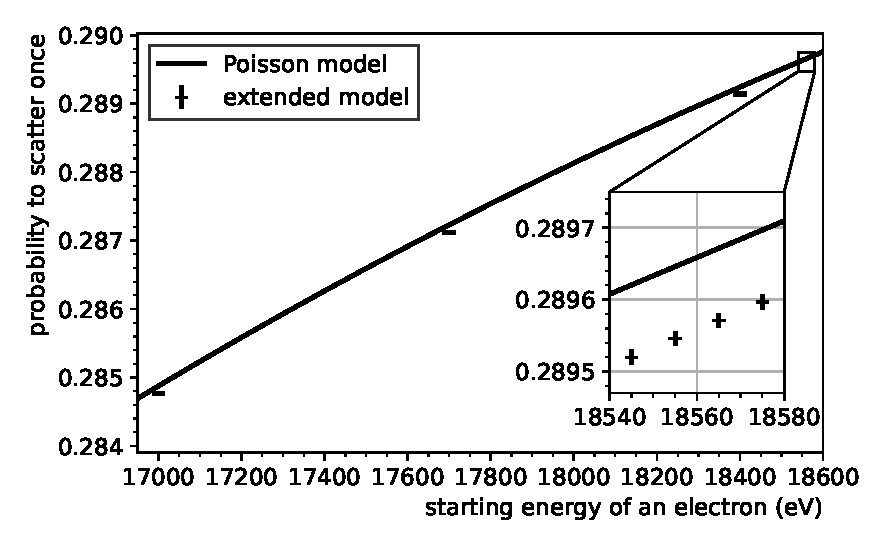
\includegraphics{chapter/energyDependentCrossSec/fig/scatProbs1PoissonAndExtended.pdf}
	\xcaption{Comparison of the Poisson and the extended model for one-fold scattering of electrons in the \glsentryshort{wgts}}{Comparison of the Poisson and the extended model for one-fold scattering of electrons in the \glsentryshort{wgts}.}{The line shows the Poisson model and the markers the extended model (see main text for a description of the models). Due to long program run times, the latter was only evaluated at a selection of energies. Furthermore, the numerical evaluation of the extended model is subject to an error of $\sim10^{-5}$ (see section~\ref{sec:eDepScatCrossSecExtendedModelNumEval}), that is depicted as uncertainty bars. The difference of the two models is $\sim10^{-4}$.}
	\label{fig:eDepScatCrossSecExtendedModelResults}
\end{figure}
For no scattering, the extended model and the Poisson model are equivalent as shown in equation~\eqref{eq:eDepScatCrossSecExtendedModelFormalismRecoveryOfPoisson}.

Figure~\ref{fig:eDepScatCrossSecExtendedModelResults} depicts the Poisson model as per equation~\eqref{eq:eDepScatCrossSecModelPoisson} and the extended model as per equation~\eqref{eq:eDepScatCrossSecExtendedModelFormalismAveragedDepScatProbs} for the probability of one-fold scattering. The difference between the two models is below $10^{-4}$.

For two-fold scattering and higher scattering multiplicities the extended model could not yet be evaluated due to the computational complexity. However an estimation based on theoretical arguments is given below.

\paragraph{Difference of the Extended and the Poisson Model for Electron Scattering}
The reasoning concerning the sign of the difference between the Poisson and the extended model is similar to the one in section~\ref{sec:eDepScatCrossSecModelPoisson} about the change of the scattering probabilities with decreasing or increasing energy: The Poisson model underestimates the total amount of scattering, because it neglects that an electron that scatters loses energy and becomes more likely to scatter again. As already shown, according to the Poisson model, electrons are expected to scatter between one and two times when traveling through the \gls{wgts} (see equation~\ref{eq:eDepScatCrossSecModelPoissonExpectedScatCount}). The extended model is more correct than the Poisson model and hence should yield an increased expected amount of scattering. Therefore, the probability for one-fold scattering should be smaller than the one given by the Poisson model (this is the case as depicted in figure~\ref{fig:eDepScatCrossSecExtendedModelResults}). For higher scattering multiplicity (which could not be calculated), the sign of the difference between the Poisson and the extended model should be the opposite. In other words, the probability of two-fold scattering as given by the Poisson model should be to low.

Also, the extended model should be a probability distribution and the sum over all scattering multiplicities should yield unity in the same manner as it does for the Poisson model (see appendix~\ref{sec:appendixEDepScatCrossSecPoissonModelProbDensityProof} for a proof that the Poisson model is a probability density). This means that for higher scattering multiplicities, the difference between the extended model and the Poisson model would have to sum up to the difference in the probability for one-fold scattering. Hence, for scattering of higher multiplicity, the absolute difference between the extended model and the Poisson model would not be able to surpass $10^{-4}$.

\paragraph{The Extended Model for Electron Scattering in Neutrino Mass Inference}
How the error of the Poisson model propagates to neutrino mass inference and whether it would introduce a significant systematic shift of the squared neutrino mass was not probed in the scope of this thesis because the current stage of the extended model is computational too demanding to be used in a fitting procedure. However, some considerations are given below:

The difference between the extended model and the Poisson model for one-fold scattering is $\sim10^{-4}$, which might be a significant scale because it is similar to the scale on which the probability for one-fold scattering changes when transitioning from an energy-independent to an energy-dependent cross section (see insets of figure~\ref{fig:eDepScatCrossSecModel}). And in the previous section~\ref{sec:eDepScatCrossSecNuMassInfThisWork}, it is shown that neglecting such an effect might lead to a systematic shift of the squared neutrino mass on the order of $\SI{e-2}{eV^2}$. Nonetheless, the difference of the extended and the Poisson model might be partly compensated by the different fit parameters such as the signal amplitude or the endpoint of the $\upbeta$ spectrum. Therefore, it was found difficult to make quantifiable assumptions.

In the following, a procedure is outlined, that might make it possible to estimate the induced systematic shift of the squared neutrino mass in a future study: One could simulate data using the Poisson model and additionally introduce an artificial negative shift on the order of $10^{-4}$ on the probability for one-fold scattering and a positive shift that is smaller than $10^{-4}$ for the probability for scattering of higher multiplicities because this should approximately resemble the extended model. The fit model can then use the Poisson model without modification. This procedure might make it possible to quantify whether there is a significant shift of the inferred squared neutrino mass caused by neglecting that electrons become more likely to scatter again if they have already scattered.

\section{Conclusion and Outlook}
\label{sec:eDepScatCrossSecConclusion}
The cross section for inelastic scattering off tritium molecules within the \gls{wgts} depends on the energy of the incident electrons. An approximated model that used the Poisson distribution was used to estimate the systematic shift on the squared neutrino mass that would be introduced if the energy dependence were neglected. The shift would be $\Delta\nuMass^2 = \SI{1.09e-2}{eV^2}$ in a \SI{30}{eV} analysis interval.

It was also shown that including the energy-dependence in neutrino mass inference via the Poisson model increases the run time of the fitting procedure by a factor of up to 140. A suggestion for an improvement of the performance via interpolation of the scattering probabilities is made in section~\ref{sec:eDepScatCrossSecModelPoissonProperties}.

The usage of the Poisson distribution underestimates the total amount of scattering, because it neglects that an electron that scatters loses energy and becomes more likely to scatter again. This does not influence the probability for no scattering. However, using the approximation of a fixed energy loss $\epsilon=\SI{12.6}{eV}$ per scattering, it could be shown that the probability for one-fold scattering would be shifted by less than $10^{-4}$. The effect on scatterings of higher multiplicities or the effect in neutrino mass inference could not be fully quantified, but an approach that might enable the quantification in the future is outlined in section~\ref{sec:eDepScatCrossSecExtendedModelDiscussion}.

The model building in this chapter was based on well argued considerations. Nonetheless, an independent cross-check is recommended. A future study might perform a Monte Carlo particle tracking simulation in order to verify the suggested models presented in this thesis.

    \def\currentRootFolder{chapter/sensitivityStudyWithPreliminaryKatrinElossModel}
\def\currentFigureFolder{\currentRootFolder/fig}

\chapter{Sensitivity Study Using an Empirical Energy Loss Model Derived from KATRIN Data for Electrons Scattering Inelastically off Deuterium}
\label{sec:katrinEloss}
A quantitative accurate description of the scattering processes of $\upbeta$ electrons within KATRIN's gaseous tritium source is of crucial importance for KATRIN's sensitivity goal. In modeling the corresponding effects, the energy loss function (see section~\ref{sec:intSpecModelResponseEloss}) plays an important role. The KATRIN Design Report states that the precision of the energy loss functions from literature is not sufficient for the KATRIN's envisaged sensitivity. It was planned to deduce a sufficiently accurate model from data taken at KATRIN~\cite{Angrik:2005ep}. In that regard, a preliminary model has successfully been established for electrons scattering off deuterium molecules based on data taken in October 2018 by a dedicated subgroup of the KATRIN collaboration. In the following, this model is referred to as the ``KATRIN model'' or the ``KATRIN energy loss model''. This preliminary energy loss model has partially improved uncertainties with respect to the model by~\cite{Aseev2000}, that is presented in the previous section~\ref{sec:intSpecModelResponseEloss}, and which was used in many previous works~\cite{Groh2015,Kleesiek2014, Kleesiek2019, SeitzM2019}. In the following, the latter model is referred to as the ``Aseev model'' after the primary author of the corresponding publication~\cite{Aseev2000}. In addition to the improved uncertainties, the KATRIN model also exhibits features not present in the Aseev model but motivated by data (see section~\ref{sec:katrinElossModel} and figure~\ref{fig:katrinElossElossModel}). 

As the energy loss function is a source of systematic uncertainties within neutrino mass inference, it is of importance to provide early feedback to the team that measures it. Beyond that, the implementation of the required statistical tools for the assessment of uncertainties into the available software frameworks is of general interest as the approach taken in the scope of this thesis may be applied to other model uncertainties, not only to the ones stemming from the energy loss function. Within the scope of this thesis, the impact on KATRIN's sensitivity by the exchange of the Aseev model for the KATRIN model was studied. In that regard, special emphasis is put on the required statistical methods. Therefore, this chapter is structured as follows: Section~\ref{sec:katrinElossModel} outlines the KATRIN model. Section~\ref{sec:katrinElossValidity} discusses the scope of the validity of this study; for example what is expected of the comparison of a model for electrons scattering off deuterium and another model for scattering off tritium molecules. Section~\ref{sec:katrinElossStatistics} introduces the statistical tools that found application in the uncertainty treatment within neutrino mass inference in this chapter. Section~\ref{sec:katrinElossModelResults} states and discusses the impact of the KATRIN model at its current stage on KATRIN's sensitivity to the neutrino mass. And section~\ref{sec:katrinElossModelOutlook} concludes and offers an outlook.


\section{The Empirical KATRIN Energy Loss Model}
\label{sec:katrinElossModel}
\newcommand{\ionEnergyDeu}{E_\mathrm{ion,D_2}}%
\begin{figure}[h!]
	\centering
	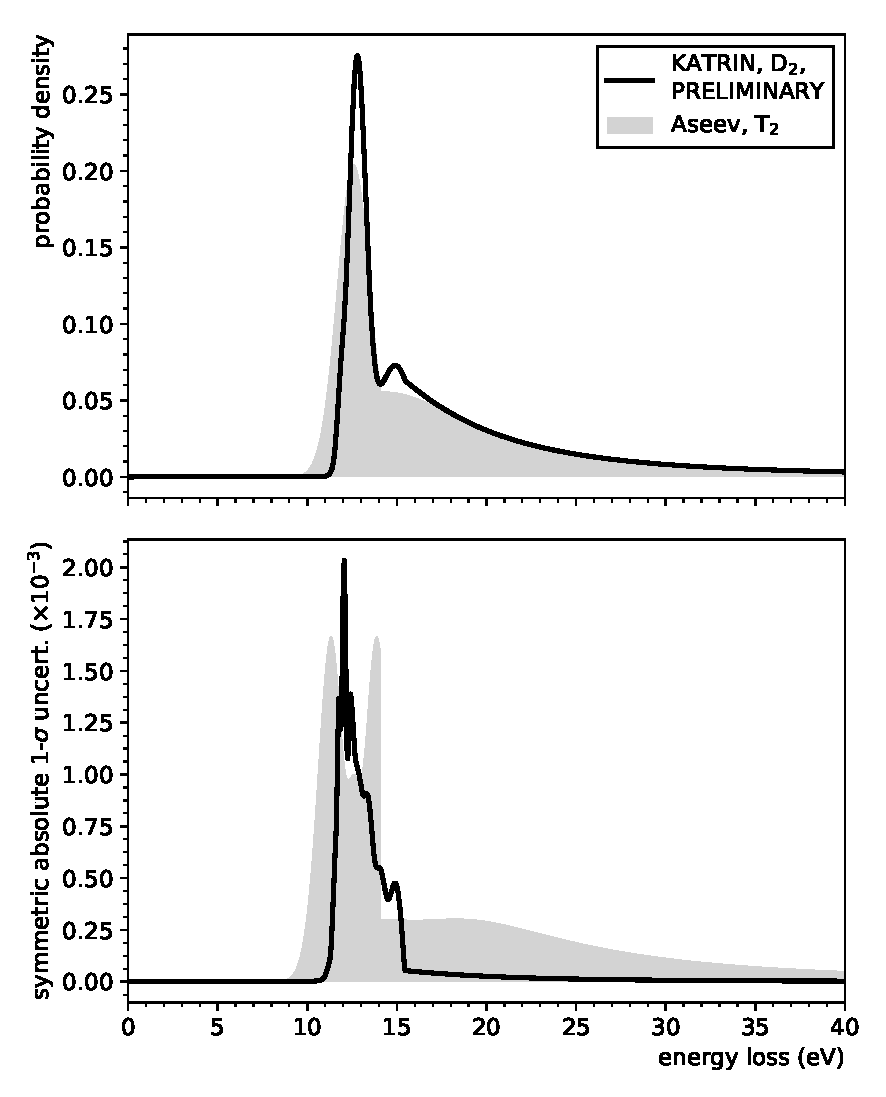
\includegraphics[width=\textwidth]{\currentFigureFolder/KATRINandAseevElossModel}
	\xcaption{The preliminary empirical KATRIN energy loss model for electrons scattering off deuterium molecules}{The preliminary empirical KATRIN energy loss model for electrons scattering off deuterium molecules.}{The black line shows the KATRIN energy loss model as established by a dedicated subgroup of the KATRIN collaboration for electrons scattering off deuterium molecules (KATRIN model). The corresponding model for scattering off tritium molecules as established by~\cite{Aseev2000} (Aseev model) is shown for comparison as a shaded area. (That the latter is plotted as area instead of as a line solely serves readability as the two functions overlap strongly.) The top panel shows the probability densities of the energy loss. The transition from the excitation peak to the ionization tail happens at the ionization energy of deuterium at $\ionEnergyDeu=\SI{15.467}{eV}$ (also refer to main text). The bottom panel shows the absolute symmetric 1-$\sigma$ uncertainties of the models. The uncertainties were obtained through uncertainty propagation via derivatives from the uncertainties of the model parameters (see figure~\ref{fig:intSpecModelAseevEloss} for the Aseev model and appendix~\ref{sec:appendixKatrinElossElossModelParams} for the KATRIN model). Correlations are respected for the KATRIN model. However, there are no published correlations for the Aseev model. The KATRIN model shows particularly improved uncertainties in the ionization tail region in comparison to the Aseev model. (KATRIN model adapted from~\cite{Hannen2019_1}.)}
	\label{fig:katrinElossElossModel}
\end{figure}
The KATRIN energy loss model was established by a dedicated subgroup of the KATRIN collaboration. It is partly of empirical nature and partly based on first principles. The model was fitted to data taken at the KATRIN experiment in October 2018. A description and a parametrization is given in the following.

\subsection{Description and Parametrization of the KATRIN Energy Loss Model}
In the preceding section~\ref{sec:intSpecModelResponseEloss}, the energy loss function $f_1(\epsilon)$ is introduced. It denotes the probability density for an energy $\epsilon$ that an electron loses when scattering once (inelastically in the current context). The KATRIN model is such an energy loss function.

The KATRIN model distinguishes two types of energy losses when an electron scatters inelastically off a gas molecule~\cite{Hannen2019_2}. The first type is the excitation of electron states within the target molecule for impact energies below the ionization energy of deuterium $\ionEnergyDeu=\SI{15.467}{eV}$~\cite{Shiner1993}. The second type is the ionization of the target molecule for impact energies above $\ionEnergyDeu$. The most probable energy losses are among the ones caused by the excitation of electronic states. In other words, the KATRIN model has a peak around these energies between approximately $\SI{12}{eV}$ and $\ionEnergyDeu$. In the following, this peak is denoted as the ``excitation peak''. Also, the part of the KATRIN model for energies above $\ionEnergyDeu$ is denoted ``ionization tail''.

The excitation peak is empirically modeled by a sum of three scaled Gaussian distributions $\mathcal{N}$. This finds inspiration in the three contributions to the vibrational molecular hydrogen states by the Lyman band, the Werner band and higher terms~\cite{Hannen2019_1} (also see~\cite{Geiger1964}). This peak $\d\sigma_\mathrm{exit}^\mathrm{phen}/\d \epsilon$  can be described by nine parameters $\nuisanceParamVec_\mathrm{eloss}$ which comprise the three scales $A_i$, means $m_i$ and standard deviations $s_i$ ($i \in \{1,2,3\}$) of the three Gaussian distributions~\cite{Hannen2019_2}
\newcommand{\katrinElossPhen}[1]{
	\frac{
		\d\sigma_\mathrm{exit}^\mathrm{phen}\giventhat*{#1}{\nuisanceParamVec_\mathrm{eloss}}
	}{
		\d \epsilon
	}
}
\begin{align}
\label{eq:katrinElossElossModelParams}
\nuisanceParamVec_\mathrm{eloss} &= 
\transp{\left(
	A_1, m_1, s_1, 
	A_2, m_2, s_2, 
	A_3, m_3, s_3
	\right)} \\
\katrinElossPhen{\epsilon} &=
\sum_{i=1}^3 A_i \cdot \mathcal{N}(\epsilon, \mu=m_i, \sigma=s_i)
\fullstop
\end{align}
The second part, the ionization tail, follows a modified version of the binary-encounter-dipole (BED) model. For the mathematical expression, the reader is referred to~\cite{Kim1994}. Here, this part will be denoted
\newcommand{\katrinElossBDE}[1]{
	\frac{
		\d \sigma_\mathrm{ion}^\mathrm{BED}(#1)
	}{
		\d \epsilon
	}
}%
\begin{equation}
	\katrinElossBDE{\epsilon}
	\fullstop
\end{equation}%
The BED model is valid for scattering off hydrogen molecules. Therefore, it depends on the ionization energy of hydrogen. The corresponding value was exchanged for the one of deuterium $\ionEnergyDeu$. Whether further modifications with regard to the difference in isotopologues are necessary is currently under investigation. Furthermore, the constant normalization factor of the BED model was removed for the following reason: The transition between the two parts, the empirical peak and the BED tail, is introduced at the ionization energy of deuterium $\ionEnergyDeu$. In order for the transition to be continuous, a scaling factor for the ionization tail is introduced
\begin{equation}
c = \left.	
	\left(
		\katrinElossPhen{\ionEnergyDeu}
	\right)
\middle/
	\left(
		\katrinElossBDE{\ionEnergyDeu}
	\right)
\right.
\fullstop
\end{equation}
Then, the full parametrization for the KATRIN model reads~\cite{Hannen2019_1}
\begin{equation}
	f_1^\mathrm{KATRIN}
	\giventhat*{\epsilon}{\nuisanceParamVec_\mathrm{eloss}} = 
	\begin{cases}
	0
	&\text{ if } \epsilon < 0 \\
	\vphantom{\scriptscriptstyle .} & \\
	\katrinElossPhen{\epsilon}
	&\text{ if } 0 \leq \epsilon \leq E_\mathrm{ion,D_2} \\
	\vphantom{\scriptscriptstyle .} & \\
	c \cdot \katrinElossBDE{\epsilon} 
	&\text{ if } \epsilon > E_\mathrm{ion,D_2}
	\end{cases}
	\fullstop
\end{equation}
Figure~\ref{fig:katrinElossElossModel} shows the KATRIN model in comparison to the Aseev model. They are not expected to be fully compatible within their uncertainties as they describe the scattering off two different hydrogen isotopologues. For a comparison of the presented KATRIN model with an energy loss model for deuterium from literature, the reader is referred to~\cite{Rodenbeck2019}. Furthermore, the parametrization of the KATRIN model comprises a second, smaller peak in the excitation region which is not present in the Aseev model. As the KATRIN model is still in its early stages, this work refrains from a detailed physical interpretation and instead focuses on uncertainty propagation. For a more detailed physical interpretation, the reader is referred to the KATRIN documents~\cite{Rodenbeck2019,Hannen2019_1,Hannen2019_2}. With respect to the uncertainties, the KATRIN model shows an improved uncertainty in the ionization tail and also in large parts of the excitation peak. How this propagates within neutrino mass inference is investigated in this chapter.

\subsection{Nuisance Parameters that Further Influence the KATRIN Energy Loss Model}
The uncertainties of the KATRIN model as evaluated at the time of writing this thesis can be divided into two sets: The KATRIN model itself comprises nine parameters. However, it was obtained in a 15-parameter fit. The other six fit parameters are correlated with the parameters of the KATRIN model and hence are not necessarily negligible with regard to uncertainty treatment. In the scope of this thesis, they were incorporated in the statistical treatment of the uncertainties. Whether they may be negligible or can be treated in a simpler fashion in future studies needs further investigation. 

For a detailed description of the full fit of the KATRIN model to the recorded data, the reader is referred to~\cite{Hannen2019_1}, but a description of the further six fit parameters is given in the following. In order to outline their meaning, an overview of the used data sets is required. Four integral spectra were recorded analogously to the described integral $\upbeta$ spectrum in chapter~\ref{sec:intSpecModel}, but with the electron gun (see section~\ref{sec:katrinExpSetupRearSection}) as electron source instead of tritium. For each data set a different deuterium column density (see section~\ref{sec:katrinExpSetupWGTS}) was set in the \gls{wgts}: \SI{0}{\percent}, \SI{15}{\percent}, \SI{50}{\percent}, \SI{100}{\percent} of the nominal column density of $\rho d = \SI{5e17}{molecules/cm^2}$. The fit model for the \mbox{\SI{15}{\percent}-measurement} was rescaled with respect to the other measurements because the respective data set underwent a different preprocessing than the others. The corresponding scaling factor $N_{\mathrm{int},15}$ was a free fit parameter. A further scaling factor $N_\mathrm{K}$ for the KATRIN model was introduced in the fit as a free parameter in order for the whole KATRIN model to keep its properties of a probability density and integrate to unity. Additionally, a fifth data set recorded at $\SI{15}{\percent}$ column density in a time-of-flight mode~\cite{Bonn1999} was fitted simultaneously. For each data set, a different expected scattering count $
\mu_{\mathrm{tof},15}, 
\mu_{\mathrm{int},15},  
\mu_{\mathrm{int},50},  
\mu_{\mathrm{int},100}$ (see equation~\ref{eq:intSpecModelExpectedScatteringCount}) was fitted, which adds four further parameters (there is no scattering for the $\SI{0}{\percent}$ measurement). In summary, the additional parameters in the fit of the KATRIN model are
\begin{equation}
\label{eq:katrinElossElossModelExtendedParams}
	\nuisanceParamVec_\mathrm{eloss+} = 
	\transp{\left(
		N_\mathrm{K},
		\mu_{\mathrm{tof},15},
		\mu_{\mathrm{int},15}, 
		\mu_{\mathrm{int},50}, 
		\mu_{\mathrm{int},100},
		N_{\mathrm{int},15}
		\right)}
	\fullstop
\end{equation}
The \gls{mle}s, the estimated standard deviations and the estimated correlation matrix of the full 15-parameter set ($\nuisanceParamVec_\mathrm{eloss}$ and $\nuisanceParamVec_\mathrm{eloss+}$) can be found in appendix~\ref{sec:appendixKatrinElossElossModelParams}. The aim of this chapter is to study the impact of the model uncertainties from these 15 parameters on KATRIN's sensitivity to the neutrino mass.

\section{Scope of the Conducted Sensitivity Study}
\label{sec:katrinElossValidity}
This section lists considerations that should be kept in mind with regard to the study presented in this chapter.

First, it should be noted that the KATRIN model as presented is still preliminary and may be subject to change because the analysis of recent measurements is still ongoing. Furthermore, the KATRIN model does not yet incorporate systematic uncertainties. Corresponding efforts for their incorporation are made at the time of writing this thesis. In that regard, a future version of the KATRIN model may exhibit larger uncertainties than the version used in this thesis. Nonetheless, once the KATRIN model is completed, the study presented in this chapter is expected to be easily repeatable because the necessary statistical tools are now readily implemented.

Furthermore, during a neutrino mass measurement, the nominal tritium purity in the~\gls{wgts} is planed to be above~\SI{95}{\percent}~\cite{Angrik:2005ep}. Here, an energy loss model for deuterium is used. Two different, but similar energy loss models are expected for the two different gas species (compare~\cite{Abdurashitov2017} and~\cite{Aseev2000}). Within the scope of this thesis, the impact on KATRIN's sensitivity from the reduction of uncertainties on the energy loss model are of primary interest. As long as the KATRIN model for scattering off deuterium molecules is sufficiently similar to a model for scattering off tritium molecules, it is a plausible approach to use it for simulations of KATRIN neutrino mass measurements (for the similarity, see figure~\ref{fig:katrinElossElossModel}). In that regard, the results for KATRIN's sensitivity derived in this chapter are expected to be meaningful - at least as a proof of concept.
\FloatBarrier
\def\currentRootFolder{chapter/sensitivityStudyWithPreliminaryKatrinElossModel/statisticalPrerequisites}
\def\currentFigureFolder{\currentRootFolder/fig}
\newcommand{\elecIndex}{\mathrm{e}}

\newcommand{\Bsource}{B^j_\mathrm{S}}
\newcommand{\BsourceAvg}{B_\mathrm{S}}
\newcommand{\zSource}{z_\mathrm{S}}
\newcommand{\thetaSource}{\theta_\mathrm{S}}
\newcommand{\thetaSourceAvg}{\theta_\mathrm{S}}
\newcommand{\Esource}{E_\mathrm{S}}
\newcommand{\Usource}{U^j_\mathrm{S}}
\newcommand{\gammaSource}{\gamma_\mathrm{S}}


\newcommand{\Bps}{B_\mathrm{PS2}}
\newcommand{\Bana}{B_\mathrm{A}}
\newcommand{\Bpinch}{B_\mathrm{P}}
\newcommand{\Bmax}{B_\mathrm{max}}
\newcommand{\Bmin}{B_\mathrm{min}}

\newcommand{\thetaMax}{\theta_\mathrm{max}}
\newcommand{\Esur}{E_\mathrm{sur}}
\newcommand{\detEff}{\epsilon_\mathrm{det}}
\newcommand{\macefilterwidth}{\Delta \mathcal{E}^j(\thetaS^j)}

\newcommand{\EtransPure}{E^j_\mathrm{tr}}
\newcommand{\Etrans}{\EtransPure(qU,\Esource,\thetaSource)}
\newcommand{\thetaTransPure}{\theta^j_\mathrm{tr}}
\newcommand{\thetaTrans}{\thetaTransPure(\Esource,qU)}

\newcommand{\As}{A_\mathrm{S}}
\newcommand{\Rbg}{R_\mathrm{bg}}


\newacronym{standardmodel}{SM}{Standard Model of Particle Physics}
\newacronym{lep}{LEP}{Large Electron Positron Collider}
\newacronym{ssm}{SSM}{standard solar model}

\section{Statistical Prerequisites}
\label{sec:katrinElossStatistics}
\subsection{Nuisance Parameters and the Profile Likelihood Method}
\label{sec:statMethodsProfileLikelihood}
Apart from the  parameters of interest $\paramVec$ (usually the squared neutrino mass), the KATRIN likelihood depends on further so-called nuisance parameters $\nuisanceParamVec$ (e.\,g. the background rate). The dimensionality may pose difficulties when deriving a confidence region for the combined parameter set. Furthermore, as indicated by the naming conventions, the dimensions of the nuisance parameters in the confidence region are not of interest. Hence, in order to derive a confidence interval with restricted dimensions, a test statistic, similar to the one in equation~\ref{eq:statMethodsLikelihoodRatio}, but that solely depends on the parameters of interest, has to be found. The following paragraph outlines, how a corresponding test statistic can be constructed using the profile likelihood method.

A corresponding derivation may start with the definition of the profile likelihood: The profile likelihood only depends on the parameters of interest $\paramVec$. Its values correspond the likelihood values evaluated at $\paramVec$ in the dimensions of the parameter of interest and maximized in the dimensions of the nuisance parameters~\cite{ReviewOfParticlePhysics}
\begin{equation}
\profLikelihood(\paramVec) = 
L(\paramVec, \hat{\hat{\nuisanceParamVec}}(\paramVec))
\comma
\end{equation}
where the double-hat indicates the maximization respectively the profiling. Also, the profile likelihood ratio can be defined~\cite{ReviewOfParticlePhysics}
\begin{equation}
\label{eq:statMethodsProfileLikelihoodRatio}
\lambda_\mathrm{p}(\paramVec) = 
\frac{\profLikelihood(\paramVec)}{\profLikelihood(\hat{\paramVec})}
\fullstop
\end{equation}
According to Wilks’ theorem~\cite{wilks1938}, the distribution of $-2\ln\lambda_\mathrm{p}(\hat{\paramVec})$, where $\hat{\paramVec}$ is the \gls{mle}, approaches a $\chi^2$ distribution in the limit of a large data sample, independent of the values of the nuisance parameters $\nuisanceParamVec$~\cite{ReviewOfParticlePhysics}. Hence, the profile likelihood ratio offers a test statistic, from which a confidence interval for the parameters of interest can be derived.

In application to a KATRIN neutrino mass measurement, the introduced formalism can be summarized as follows: The profile likelihood~\eqref{eq:statMethodsProfileLikelihoodRatio} is a measure (test statistic) for whether a hypothesized squared neutrino mass has to be rejected given the KATRIN data. Furthermore, analogously to section~\ref{sec:statMethodsUncertaintyIntervalsConfidence}, this allows for the derivation of a confidence interval for the squared neutrino mass. It should be noted, however, that this method requires an extrapolation of the likelihood to nonphysical negative squared neutrino masses~\cite{Kleesiek2014}.


\subsection{Sensitivity from  the Profile Likelihood Method}
In the scope of this thesis, the sensitivity on the neutrino mass is evaluated using the profile likelihood method (section~\ref{sec:statMethodsProfileLikelihood}) in order to account for nuisance parameters and especially their correlations. The profile likelihood method was also used in~\cite{Kleesiek2014} for a KATRIN standard 4-parameter fit (section~\ref{sec:statMethodsProfileLikelihood}). The obtained value for $\statUncert$ is plotted and can be extracted to be between \SIrange[range-phrase=--]{0.0155}{0.0165}{eV^2} which is in agreement with the result $\statUncert=\SI{0.0162}{eV^2}$ from ensemble testing (see table~\ref{tab:statMethodsSensitivityFromEnsembleTests}). ``In case of the standard 4 parameter fit, the confidence intervals calculated from ensemble tests are in very good agreement with alternative methods [...], including likelihood ratio intervals (profile likelihood method)'' Kleesiek, page 160, profile likelihood, optimized mtd, uncertainty on suqred mnu $0.01494 eV^2$.



\subsection{Combination of Commissioning and Neutrino Mass Measurements}
If two measurements share a set of parameters $\paramVecShared$, but have additionally an individual set of parameters $\paramVec_1$ and $\paramVec_2$ and different sets of observations a combined likelihood is given by the product of the single likelihoods $L_1$ and $L_2$
\begin{equation}
-2\ln L(\paramVecShared, \paramVec_1, \paramVec_2) =  
-2\ln L_1(\paramVecShared, \paramVec_1)
-2\ln L_2(\paramVecShared, \paramVec_2)
\fullstop
\end{equation}
In the case of KATRIN the first measurement could be sensitive to the neutrino mass whereas say the second measurement could have been a calibration using the electron gun and be sensitive to parameters of the response function \eqref{eq:SSCresponse}. Combining both likelihoods would incorporate the uncertainties on the parameters of the response function in the neutrino mass determination. Currently, no software framework exists that allows the construction of combined likelihoods of KATRIN neutrino mass and calibration measurements. Instead the following approximation can be made. The calibration measurement is evaluated independently and one obtains estimates $\hat{\paramVec}_\mathrm{s,2}$, and an estimated covariance matrix $\hat{V}_\mathrm{s,2}$ for all components of $\paramVecShared$ that the calibration measurement is sensitive to. These can in turn be used to approximate the likelihood $L_2$ at least in the dimension of $\paramVecShared$. A choice that stands to reason for the approximation of $L_2$ is a multivariate Gaussian distribution. For the purpose of parameter inference through minimization $-2\ln L_2$ needs only to be accurately approximated around its minimum. The choice of a multivariate Gaussian distribution corresponds a symmetric approximation of $-\ln L_2$ around its minimum by a parabola. The KATRIN likelihood for a combination of a neutrino mass and a calibration measurement then reads
\begin{equation}
\begin{split}
\label{eq:penalizedLikelihood}
-2\ln L(\paramVecShared, \paramVec_1, \paramVec_2) &\approx
-2\ln L^\prime(\paramVecShared, \paramVec_1) \\ &=
\underbrace{
	\chi^2(\paramVecShared, \paramVec_1)
	\vphantom{(\paramVecShared - \hat{\paramVec}_\mathrm{s,2})^{\mathsf{T}}}
}_{(1)}
+
\underbrace{
	(\paramVecShared - \hat{\paramVec}_\mathrm{s,2})^{\mathsf{T}}
	\hat{V}_\mathrm{s,2}^{-1}
	(\paramVecShared - \hat{\paramVec}_\mathrm{s,2})
}_{(2)} +\; 
\mathrm{ constants}\\ &=
\chi^2(\paramVecShared, \paramVec_1) 
-2\ln \mathcal{N}(\paramVecShared, \hat{\paramVec}_\mathrm{s,2}, \hat{V}_\mathrm{s,2}^{-1}) +
\mathrm{ constants}
\end{split}
\end{equation}
Here, $(1)$ is the chi-square expression \eqref{eq:katrinChi2} where the $\paramVecShared$ and $\paramVec_1$ can be written as one combined parameter vector $\paramVec$ for a neutrino mass measurement. And $(2)$ resembles the negative log likelihood of the calibration measurement approximated by a multivariate Gaussian distribution. Terms having a form like $(2)$ are also sometimes called ``pull terms'' or ``likelihood penalties''. In the minimization process they ``pull'' the parameters $\paramVecShared$ towards $\hat{\paramVec}_\mathrm{s,2}$ respectively ``penalize''/increase the negative log likelihood if $\paramVecShared$ and $\hat{\paramVec}_\mathrm{s,2}$ differ.


\newcommand{\CombLmax}{-2\ln L(\hat{\paramVec}_\mathrm{s}, \hat{\paramVec}_1)}
The chi-square term $(1)$ is a sum of $n$ standard normal distributed random variables. Hence, as discussed, a likelihood only composed of the chi-square term $(1)$ offers a goodness-of-fit criteria via the the Pearson chi-square statistic. Note that for the combined likelihood this criteria might not hold. Two special cases can be considered where the chi-square characteristics hold approximately: First, the neutrino mass measurement, term $(1)$, is not sensitive to the shared parameters $\d \chi^2(\paramVecShared, \paramVec_1) /\d \paramVecShared \approx 0$. Then the \gls{mle} for the shared parameters will match the \gls{mle} by the calibration measurement $\hat{\paramVec}_\mathrm{s} = \hat{\paramVec}_{\mathrm{s},2}$ and term $(2)$ will be 0. The combined likelihood evaluated at the \gls{mle} $\CombLmax$ then follows a chi-square distribution with $n-\dim\paramVec_1-\dim\paramVecShared$ degrees of freedom. Second, if the neutrino mass measurement is sensitive to some shared parameters $\d \chi^2(\paramVecShared, \paramVec_1) /\d \paramVecShared \neq 0$, then one might argue, that term $(2)$ evaluated at the \gls{mle} $\hat{\paramVec}_\mathrm{s} \neq \hat{\paramVec}_{\mathrm{s},2}$ is a sum of standard normal distributed random variables. If this holds, the combined likelihood evaluated at the \gls{mle} $\CombLmax$ follows a chi-square distribution with $n-\dim\paramVec_1$ degrees of freedom.


For example, a standard KATRIN 3-year neutrino mass measurement is not at all sensitive to parameters of the energy loss function \eqref{eq:nonAveragedResponse}. Hence, adding a corresponding term $(2)$ from a designated energy loss measurement will not influence the chi-square characteristics. However, a standard KATRIN neutrino mass measurement is even after a short measurement time sensitive to the gas column density \eqref{eq:columnDensity}. Adding a corresponding term $(2)$ from (a naturally more sensitive) monitoring measurement would influence the   


\todo{Add plots from ensemble test that proof statements.}

\subsection{Extension of the KaFit Software Framework}
\label{sec:statLikelihoodExtImpl}
The likelihood $L(\paramVec)$ can be multiplied by a function $g(\paramVec)$
\begin{equation}
\label{eq:likelihoodExtension}
-2\ln L^\prime(\paramVec) = -2\ln L(\paramVec) -2\ln g(\paramVec)
\fullstop
\end{equation}
This procedure may have different interpretations and usage scenarios. E.g. a comparison with \eqref{eq:posterior} shows, if $g$ is a prior probability distribution, $L^\prime$ becomes a non-normalized posterior distribution that can be used in a Bayesian analysis. A further interpretation is given in section \ref{sec:combinationOfMeasurements}.
\label{sec:combinationOfMeasurements}

KaFit allowed to choose $g$ in \ref{eq:likelihoodExtension} as a product of one-dimensional Gaussian distributions. Within this thesis the software was extended to allow products of other functions. Three function types were explicitly made available through a configuration file.
\begin{enumerate}
	\item A reimplementation of a one-dimensional Gaussian distribution: The reimplementation was necessary to conveniently enable the combination of function types.
	\item A multivariate Gaussian distribution: This enables the treatment of uncertainties quantified by calibration or monitor measurements as described in section \ref{sec:combinationOfMeasurements}. It can also be used as a prior distribution in a Bayesian analysis. Particularly, correlations can be respected.
	\item A one-dimensional probability density, that is constant in the square root of a parameter, if it is positive and 0 otherwise:
	\begin{equation}
		g(\theta) =
		\begin{cases}
		0 &\text{ if } \theta \leq 0 \\
		\text{constant} \cdot \frac{1}{\sqrt{\theta}} &\text{ if } \theta > 0
		\end{cases}
		\fullstop
	\end{equation}
	 This can be used as a uniform prior on the neutrino mass ($\theta=m_\nu^2$). Formerly, it was only possible to use a uniform prior on the squared neutrino mass. A derivation of the form of $g$ can be found in appendix \ref{sec:appStatisticPriorOnNu2}.
\end{enumerate}
An example on how to configure KaFit using the new feature is given in appendix \todo{Add appendix}.


\def\currentRootFolder{chapter/sensitivityStudyWithPreliminaryKatrinElossModel}
\def\currentFigureFolder{\currentRootFolder/fig}
\FloatBarrier
\section{Deduced Sensitivity to the Neutrino Mass}
\label{sec:katrinElossModelResults}
This section lists the results of the study on the impact from the uncertainties of the KATRIN model on KATRIN's sensitivity. The results are compared to the impact of the uncertainties from the Aseev model. The sensitivity study was conducted using a mathematical model of a KATRIN neutrino mass measurement as described in chapter~\ref{sec:intSpecModel} using a nominal configuration according to the KATRIN Design Report~\cite{Angrik:2005ep} with a neutrino mass of \SI{0}{eV} and a measurement time of three years. Correspondingly, the SSC and KaFit modules were used (see section~\ref{sec:statMethodsKaFitSSC}). The full configuration of the study can be found in appendix~\ref{sec:appendixKatrinElossSSCConfig}. The uncertainties of the KATRIN respectively the Aseev model were respected as described in section~\ref{sec:katrinElossStatisticsCombMeasurements} about the combination of a neutrino mass and a calibration measurement. The confidence interval for the squared neutrino mass was extracted via the profile-likelihood method as described in section~\ref{sec:katrinElossStatisticsProfileLikelihood}.

Section~\ref{sec:katrinElossModelResultsAsimov} presents the study using an Asimov data set. And section~\ref{sec:katrinElossModelResultsEnsemble} presents the same results as obtained through an ensemble test (for the relation of these two approaches see section~\ref{sec:katrinElossStatisticsAsimov}).
\subsection{Sensitivity from an Asimov Data Set}
\label{sec:katrinElossModelResultsAsimov}
\begin{figure}[t]
	\centering
	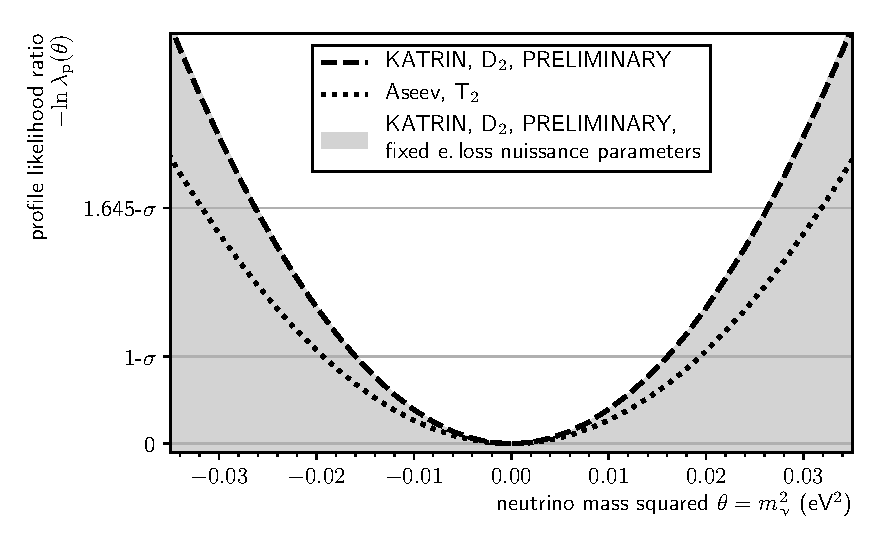
\includegraphics[width=\textwidth]{\currentFigureFolder/profileLikelihoodKATRINandAseev.pdf}
	\xcaption{Profile-likelihood ratio of a KATRIN measurement from an Asimov data set}{Profile-likelihood ratio of a KATRIN measurement  from an Asimov data set.}{The graph shows the profile-likelihood ratio $\lambda_\mathrm{p}$ for three different cases with different uncertainties: using the KATRIN model (dashed line), the Aseev model (dotted line) or the ``statistics only'' case (shaded area). For a description of the different cases, the reader is referred to the main text. (That the ``statistics only'' case is plotted as an area instead of as a line solely serves readability because a line would overlap with the line for the KATRIN model.) The \gls{mle} recovers the true simulated squared neutrino mass of \SI{0}{eV^2} with a corresponding likelihood ratio (and profile likelihood ratio) of 1 ($\Rightarrow-\ln\lambda_\mathrm{p}(\hat{\theta})=0$). The horizontal $s$-$\sigma$ lines are drawn at $s^2/2$ as per equation~\eqref{eq:statMethodsConfidenceContour}. Their intersections with $-\ln\lambda_\mathrm{p}$ mark the confidence intervals for the neutrino mass at \SI{68}{\percent} respectively \SI{90}{\percent} confidence level. The width of the two intervals indeed relate through the factor 1.645 due to the parabolic shape of $-\ln\lambda_\mathrm{p}$. It is apparent, that the uncertainties of the KATRIN model hardly have an impact compared to the ``statistics only'' case (also see table~\ref{tab:katrinElossModelResultsAsimov}). The corresponding profile likelihoods are almost equal.}
	\label{fig:katrinElossResultsProfileLikelihood}
\end{figure}
The following three cases were investigated using an Asimov data set:\mynobreakpar
\begin{enumerate}
	\item The simulation- and fit-model use the KATRIN energy loss model, but it was assumed to be without uncertainties. In other words, only the four parameters of a nominal KATRIN-neutrino-mass fit (see section~\ref{sec:statMethodsStandardFit}) were treated as free parameters and the parameters of the KATRIN energy loss model were fixed to their best estimates. In the following, this is referred to as the ``statistics only'' case.
	\item The simulation- and fit-model use the KATRIN energy loss model, and all its parameters were treated as free in order to incorporate the uncertainties of the KATRIN model, which results in a 19-parameter fit.
	\item The simulation- and fit-model use the Aseev model, and all its parameters were treated as free in order to incorporate the uncertainties of the Aseev model, which results in a nine-parameter fit.
\end{enumerate}
Figure~\ref{fig:katrinElossResultsProfileLikelihood} shows the corresponding profile-likelihood ratios and table~\ref{tab:katrinElossModelResultsAsimov} lists the extracted confidence intervals and obtained sensitivities. The ``statistics only'' case can be compared to the results of former works listed in table~\ref{tab:statMethodsSensitivityFromEnsembleTests}. Here, a $\sim\SI{4e-4}{eV^2}$ smaller statistical uncertainty on the squared neutrino mass is obtained compared to the results by~\cite{Kleesiek2014, Hoetzel2012}. This is mainly due to the fact, that in the study presented in this chapter a detection efficiency of \SI{95}{\percent} was used, whereas the other works used~\SI{90}{\percent}. In reference to the extrapolation of the likelihood to negative squared neutrino masses as discussed in section~\ref{sec:statMethodsUncertaintyIntervalsConfidence}, it becomes apparent, that the extrapolation is slightly asymmetric.

Under the restrictions listed in section~\ref{sec:katrinElossValidity}, the following conclusions can be drawn:
\begin{itemize}
	\item Treating the parameters of the KATRIN model as free parameters in order to avoid systematic shifts of the squared neutrino mass and constraining them as described in section~\ref{sec:katrinElossStatisticsCombMeasurements} about the combination of a calibration and neutrino mass measurement results in a enlarged statistical uncertainty (\SI{68}{\percent} C.L.) for the squared neutrino mass
	\begin{equation*}
		\Delta \sigma_\mathrm{tot}(\nuMass^2) = \SI{1.2e-4}{eV^2}
		\fullstop 
	\end{equation*} 
	This enlargement is negligible with respect to the KATRIN systematic budget.
	\item Using the KATRIN model at its current stage yields an improvement of~\SI{10}{meV} in sensitivity to the neutrino mass compared to using the Aseev model. It should be noted that the presented study only investigates the uncertainties of said models, but does not make further statements about their applicability. In other words, there may be reasons to transit to the KATRIN model beyond the improvement of the sensitivity. For example, the inclusion of the second peak (see figure~\ref{fig:katrinElossElossModel}) in the energy loss function may proof to be more correct.
	\item The logarithm of the profile-likelihood ratio has a parabolic shape, which translates to a Gaussian shape for the likelihood. This justifies the usage of the factor $1.645$ to convert a confidence interval of~\SI{68}{\percent} confidence level into one of~\SI{90}{\percent}.
\end{itemize}

\begin{table}[t]
	\centering
	\xcaption{Neutrino mass confidence intervals and sensitivities obtained from an Asimov data set}{Neutrino mass confidence intervals and sensitivities obtained from an Asimov data set.}{The table lists values that can be extracted from the profile-likelihood ratio depicted in figure~\ref{fig:katrinElossResultsProfileLikelihood} for the three conducted studies: the ``statistics only'' case and respecting the uncertainties from the KATRIN and the Aseev model. The following quantities are listed: the lower bound of the confidence interval (\SI{68}{\percent} C.L.) on the squared neutrino mass $l(\nuMass^2)$, the upper bound $u(\nuMass^2)$, half the width of the interval $\sigma_\mathrm{tot}(\nuMass^2)$ and KATRIN's sensitivity on the neutrino mass as per equation~\eqref{eq:statMethodsSensitivity}. For the calculation of the sensitivity an additional systematic budget of $\SI{0.017}{eV^2}$ was included (see section~\ref{sec:statMethodsSensitivtyFromEnsemble}).}
	\begin{tabular}{lrrrr}
		\toprule
		\makecell[tr]{} &
		\makecell[tr]{$l(\nuMass^2)$ \\ (\SI{e-2}{eV^2})} & 
		\makecell[tr]{$u(\nuMass^2)$ \\ (\SI{e-2}{eV^2})} & 
		\makecell[tr]{$\sigma_\mathrm{tot}(\nuMass^2)$ \\ (\SI{e-2}{eV^2})} &
		\makecell[tr]{$S_{\nuMass}(\SI{90}{\percent})$ \\ (\SI{}{meV})}  
		\\
		\hline
		``statistics only'' & -1.586 & 1.592 & 1.589 & 196 \\
		KATRIN model & -1.598 & 1.604 & 1.601 & 196 \\
		Aseev model & -1.931 & 1.939 & 1.935 & 206 \\
		\bottomrule
	\end{tabular}
	\label{tab:katrinElossModelResultsAsimov}
\end{table}

\subsection{Cross-Check and Extension of the Asimov Data Set via Ensemble Testing}
\label{sec:katrinElossModelResultsEnsemble}
An ensemble of 4046 KATRIN neutrino mass measurements with a true neutrino mass of~\SI{0}{eV} was simulated using the KATRIN energy loss model and incorporating its uncertainties in the same manner as for the Asimov data set described in the last section~\ref{sec:katrinElossStatisticsAsimov}. However, as opposed to the Asimov data set, in the simulation of the ensemble, the detector counts were fluctuated according to Poissonian statistics. Several aspects were investigated as listed below:

\paragraph{Test of Coverage}
The extraction of a confidence interval via the profile-likelihood method as done in the previous section~\ref{sec:katrinElossStatisticsAsimov} for the Asimov data set should per construction yield a coverage probability of \SI{68.2}{\percent}. But if all conditions are met for this to hold has to be justified. Either a theoretical argument can be given or it can simply be put to the test. In the scope of this thesis, the approach per test was chosen. In other words, \SI{68.2}{\percent} of the obtained confidence intervals in the conducted ensemble test should cover the true simulated squared neutrino mass of~\SI{0}{eV^2}. The obtained coverage is \SI{67.6}{\percent} as illustrated in figure~\ref{fig:katrinElossResultsCoverage}. The slight undercoverage on the $10^{-3}$ scale may stem from a limited ensemble test size. Furthermore, it must be emphasized that here the likelihood of the measurement of the KATRIN energy loss model is approximated by a multivariate normal distribution and does not fluctuate in the presented ensemble test. For the result to have full validity, the measurement of the KATRIN energy loss model has to be simulated along with the KATRIN neutrino mass measurement. This may be the aim of a future analysis.

\paragraph{Chi-Square Characteristics}
The combined likelihood of a neutrino mass and a calibration measurement evaluated at the \gls{mle} $-2\ln L(\hat{\paramVec})$ might not follow the chi-square statistic as mentioned in section~\ref{sec:katrinElossStatisticsCombMeasurements}. Figure~\ref{fig:katrinElossStatisticsChi2} shows the obtained distribution of $-2\ln L(\hat{\paramVec})$ in the conducted ensemble test. An \gls{mtd} with 41 retarding potentials was used. Hence, there are 41 summands in the likelihood for the KATRIN neutrino mass measurement. In the combined likelihood, there are additional 15 summands to approximate the likelihood of the measurement of the KATRIN energy loss model. In total, there are 19 fit parameters, four for the nominal KATRIN neutrino mass fit (see section~\ref{sec:statMethodsStandardFit}) and 15 in order to incorporate the uncertainties of the KATRIN model. Thus, the hypothesis stands to reason that the obtained distribution follows a chi-square distribution with $41+15-19=37$ degrees of freedom. A corresponding Kolmogorov–Smirnov test yields a $p$-value of $p=\SI{6e-6}{}$. In other words, this hypothesis has to be rejected with a significance of $4\sigma$. Repeating the test for 38 respectively 39 degrees of freedom yields $p=\SI{0.14}{}$ respectively $p=\SI{1e-14}{}$. Hence, a chi-square distribution of 38 degrees of freedom may not be rejected. This is important because it means that the chi-square statistic can not necessarily be used as a measure for goodness-of-fit when incorporating the uncertainties of the KATRIN energy loss model into the neutrino mass inference in the way described in this thesis. Or, at least, one has to be careful about the choice of degrees of freedom.

\begin{figure}[th]
	\centering
	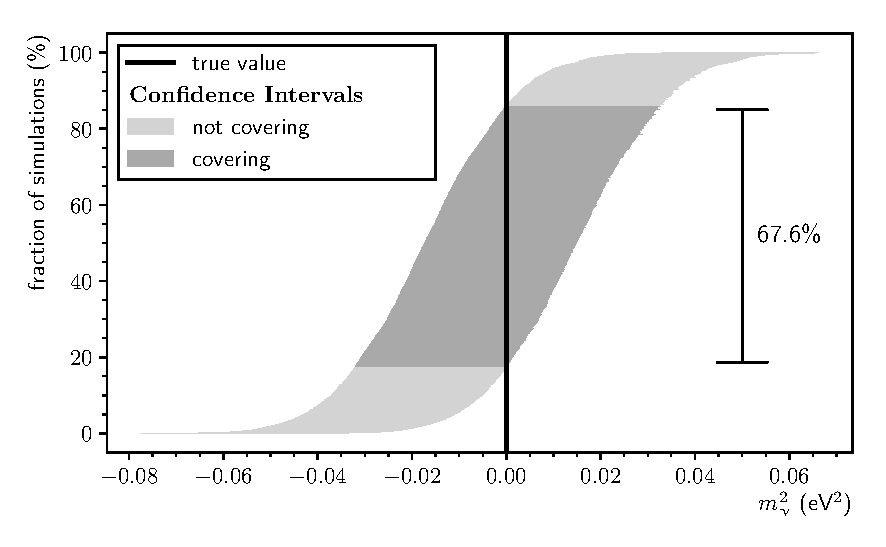
\includegraphics[width=\textwidth]{\currentFigureFolder/coverage.pdf}
	\xcaption{Test of coverage for the ensemble of confidence intervals obtained in the sensitivity study using the KARTRIN energy loss model}{Test of coverage for the ensemble of confidence intervals obtained in the sensitivity study using the KARTRIN energy loss model.}{The graph illustrates the coverage probability. An ensemble of 4046 KATRIN neutrino mass measurements with a true squared neutrino mass of~\SI{0}{eV^2} was simulated. For each simulated measurement a confidence interval was constructed using the profile-likelihood method. The obtained confidence intervals were sorted by their lower limit and plotted stacked which yields the gray band. The confidence intervals that cover the true value are depicted in dark gray, while the ones that do not cover the true value are depicted in light gray. In total~\SI{67.8}{\percent} coverage is obtained. In the limit of an infinite ensemble size, a coverage of~\SI{68.2}{\percent} would be expected per construction (also refer to the main text for a limitation of this statement). It should also be noted, that there is little fluctuation in the width of the confidence intervals, which illustrates the representative qualities of an Asimov data set.}
	\label{fig:katrinElossResultsCoverage}
\end{figure}

\paragraph{Representative Qualities of the Asimov Data Set}
The estimated mean and standard deviation of the distribution of the  confidence intervals (\SI{68}{\percent} C.L.) as obtained by the ensemble test is $\hat{\sigma}_\mathrm{tot}(\nuMass^2)=\SI{1.599\pm0.013e-2}{eV^2}$ in agreement with the one obtained through the Asimov data set in table~\ref{tab:katrinElossModelResultsAsimov}. Furthermore, the median confidence interval $\tilde{\sigma}_\mathrm{tot}(\nuMass^2)=\SI{1.598e-2}{eV^2}$ should recover the one of the Asimov data set~\cite{Cowan2011}, which is indeed the case on the \SI{e-5}{eV^2} level. This verifies the Asimov data set as representative for the study on the KATRIN energy loss model presented in this chapter.

\begin{figure}[t]
	\centering
	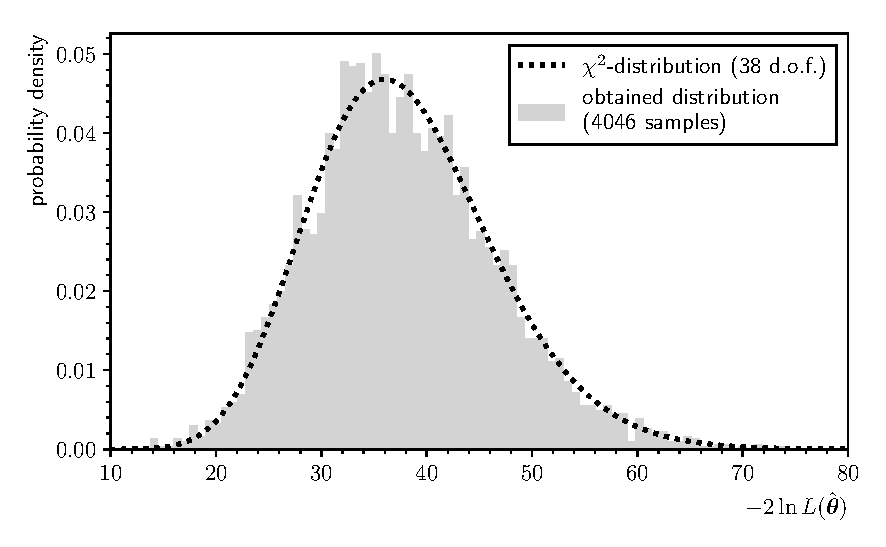
\includegraphics[width=\textwidth]{\currentFigureFolder/katrinElossChi2Distribution.pdf}
	\xcaption{Chi-square distribution for the simulated ensemble of neutrino mass measurements obtained in the sensitivity study using the KATRIN energy loss model}{Chi-square distribution for the simulated ensemble of neutrino mass measurements obtained in the sensitivity study using the KATRIN energy loss model.}{An ensemble of 4046 KATRIN neutrino mass measurements was simulated. The histogram shows the obtained distribution of the likelihood $L$ evaluated at the~\gls{mle}~$\hat{\theta}$. The obtained distribution may follow a chi-square distribution with 38 degrees of freedom. For details the reader is referred to the main text.}
	\label{fig:katrinElossStatisticsChi2}
\end{figure}
\FloatBarrier
\section{Conclusion and Outlook}
\label{sec:katrinElossModelOutlook}
A general statistical framework was developed that enables the incorporation of model uncertainties into parameter inference. It was used to show that the uncertainties of the KATRIN energy loss model at its current preliminary stage would increase the statistical uncertainty on the squared neutrino mass by $\Delta \sigma_\mathrm{tot}(\nuMass^2) = \SI{1.2e-4}{eV^2}$, which is negligible given the KATRIN systematic budget. Furthermore, it was shown, that Asimov data sets of the presented kind may reasonably be assumed to be representative for an ensemble of neutrino mass measurements. Also, it was demonstrated, that precautions have to be taken, when using the chi-square statistic as a measure for goodness-of-fit at the same time as incorporating ``pull terms''. 

The paragraphs below present possible follow-up studies as an outlook:

It is recommended to repeat the presented study once the KATRIN energy loss model is available in its final version and also available for electrons scattering off tritium molecules.

Also, a general routine may be established that derives a test statistic for the goodness-of-fit from simulated ensembles where the chi-square statistic may not hold. 

Furthermore, it would be of interest to develop a software framework that can treat a KATRIN electron gun measurement in combination with a KATRIN neutrino mass measurement in order for the presented ``pull term''-approximation to become obsolete.
    \chapter{Conclusion}
\label{sec:conclusion}
In the scope of this thesis, two aspects concerning the inelastic scattering of electrons in the \gls{wgts} were investigated:

\paragraph{Energy-dependence of the Inelastic Scattering Cross Section}
In section~\ref{sec:eDepScatCrossSecModel}, models that incorporate the dependence of the inelastic scattering cross section on the energy of incident electrons were presented. An approximation was used when modeling the probability for severalfold scattering via a Poisson distribution. Whether this approximation needs refinement was not ultimately clarified.

Using the approximated model, strong indications were found, that the energy-dependence should not be neglected in neutrino mass inference as this would shift the inferred neutrino mass by 	$\Delta\nuMass^2 = \SI{1.09e-2}{eV^2}$ when using the design KATRIN analysis interval of \SI{30}{eV}. However, an independent cross-check of the suggested models is recommended.

\paragraph{Statistical Methods and the KATRIN Energy Loss Model}
The profile-likelihood-method and the usage of an Asimov data set were reviewed in the context of uncertainty propagation from the KATRIN energy loss model to neutrino mass inference. Both concepts are only applicable in the large sample limit. An ensemble test showed that this limit is given. It was found that the current uncertainties on the KATRIN energy loss model do not influence KATRIN's sensitivity significantly. This result is, however, preliminary as the KATRIN energy loss model is not yet final. Nonetheless, the study may serve as a proof-of-concept and is expected to be repeatable with less effort, as the corresponding statistical tools were implemented in the KaFit software framework. 


    \Appendix
    \chapter*{\appendixname} \addcontentsline{toc}{chapter}{\appendixname}
    \section{Energy-Dependent Model of the Probability for Electron Scattering within the \gls{wgts}}
\label{sec:appendixEDepScatCrossSecExtendedModel}
Section~\ref{sec:eDepScatCrossSecModel} introduces a model for the probability of electron scattering within the \gls{wgts} using the Poisson distribution. As explained, depending on the required accuracy, the conditions for using a Poisson distribution might be violated. Section~\ref{sec:appendixEDepScatCrossSecExtendedModelFormalism} introduces a model beyond the description via a Poisson distribution. Its evaluation was done numerically which demanded a trade-off between accuracy and run time. The latter is assessed in section~\ref{sec:appendixEDepScatCrossSecExtendedModelNumEval}.
\subsection{Modeling}
\label{sec:appendixEDepScatCrossSecExtendedModelFormalism}
In the following, a model for for the probability of electron scattering within the \gls{wgts} that depends on the electrons energy is derived. The difficulty lies in the fact, that an electron that scatters looses energy and hence its probability to scatter a second time is different from the first time. The presented model is inspired by a model given in~\cite{Groh2015}, that treats a similar effect for a change of an electron's pitch angles due to scattering. 

The aim is to derive an expression $\bar{P}^{\star}_l(\Esource)$ that denotes the probability of $l$-fold scattering for a $\upbeta$ electron with a starting energy $\Esource$ averaged over all starting positions and pitch angles assuming a fixed energy loss $\epsilon$ per scattering.

The expected amount of scatterings for a $\upbeta$ electron when traveling  through the whole \gls{wgts} volume of length $d$ filled with a gas of constant density $\rho$ is (see equation~\ref{eq:intSpecModelExpectedScatteringCount})
\begin{equation}
    \mu(E,\thetaSource) =
    \frac{\sigma(E)\rho d}{\cos\thetaSource},
\end{equation}
where $E$ denotes the electron's kinetic energy; $\thetaSource$ the starting pitch angle; and $\sigma(E)$ the energy dependent scattering cross section.

In the developed model, the volume of the \gls{wgts} is divided into $N$ slices of equal width $w=L/N$. $N$ is chosen sufficiently large that the probability for a $\upbeta$ electron to scatter twice within one slice is essentially zero. Then, for large $N$ the probability to scatter within one slice is $\mu(E,\thetaSource)/N$. The probability not to scatter within $n \leq N$ slices is
\begin{equation}
    p_0(E,\thetaSource,n) =
    \left(
        1-\frac{\mu(E,\thetaSource)}{N}
    \right)^n
    \fullstop
\end{equation}
Using the well known limit for the Euler constant, one obtains for $n=N$ and $N\rightarrow\infty$ that $p_0$ is a Poisson distribution with expectation $\mu$ evaluated at 0 
\begin{align}
    \lim_{N\rightarrow\infty} 
    p_0(E,\thetaSource,N) =
    \lim_{N\rightarrow\infty} 
    \left(
        1-\frac{\mu(E,\thetaSource)}{N}
    \right)^N =
    \mathrm{e}^{-\mu(E,\thetaSource)}
    \fullstop
\end{align}
In other words, for no scattering, the Poisson model for the scattering probabilities as described in section~\ref{sec:eDepScatCrossSecModel} is recovered.

Assuming a constant energy loss per scattering of $\epsilon$ the probability to scatter $l$ times within $n<N$ slices can be expressed recursively
\begin{equation}
	\label{eq:appendixEDepScatCrossSecExtendedModelFormalismCore}
    p_l(E,\thetaSource,n) =
    \underbrace{
        \sum_{k=l}^{n}
    }_{(4)}
    \underbrace{
        p_{l-1}(E,\thetaSource,k-1)
        \vphantom{\sum_{k=l}^{n}}
    }_{(1)}
    \underbrace{
    \left(
        1-p_0(E-(l-1)\epsilon,\thetaSource,1)
    \right)
    \vphantom{\sum_{k=l}^{n}}
    }_{(2)}
    \underbrace{
        p_0(E-l\epsilon,\thetaSource,n-k)
        \vphantom{\sum_{k=l}^{n}}
    }_{(3)}
    \fullstop
\end{equation}
The idea behind this expression is the following: One imagines an electron with an energy $E$ that travels through $n$ \gls{wgts} slices, scatters $l$ times in total and once in the $k$th slice. Hence, it must have scattered $l-1$ times in the $k-1$ slices and must not scatter in the $n-k$ slices to follow. In that regard, the above terms have the following meaning:
\begin{enumerate}[(1)]
    \item Probability to scatter $l-1$ times within $k-1$ slices with a kinetic energy of $E$.
    \item Probability to scatter once within the $k$th slice with a kinetic energy of $E-(l-1)\epsilon$.
    \item Probability not to scatter within the remaining $N-k$ slices.
    \item Sum over all slices $k$ where the electron could scatter the last time. The sum starts at $l$ because the probability to scatter $l-1$ times within less than $k=l-1$ slices (term (1)) is 0 because of the made assumption, that in the limit of large amount of slices $N$ an electron does not scatter twice within one very narrow slice.
\end{enumerate}
The probability to scatter $l$ times can be averaged over all starting positions
\begin{equation}
    \label{eq:appendixEDepScatCrossSecExtendedModelFormalismZAverage}
    \bar{p}_l(E,\thetaSource) = 
    \frac{1}{N}
    \sum_{\nSource=1}^{N} p_l(E,\thetaSource,\nSource) \approx
    \frac{1}{d}
    \int_{0}^{d}
        p_l(E,\thetaSource,
            \left\lceil N \frac{\zSource}{d}\right\rceil
        )
    \d \zSource
    \fullstop
\end{equation}
Here, the averaging sum is approximated by an integral as this helps cutting down on run time in a numerical evaluation. This is due to the fact, that in a numerical evaluation a large number $N$ ($\sim10^5$) of slices has to be chosen and the sum would have many terms. However, a numerical integration can achieve an accurate result with a smaller set of supporting points (see subsequent section~\ref{sec:appendixEDepScatCrossSecExtendedModelNumEval}). 

In the formal expression, the limit $N\rightarrow\infty$ can be applied
\begin{equation}
  P^{\star}_l(\Esource,\thetaSource) = 
    \lim_{N\rightarrow\infty} \bar{p}_l(\Esource,\thetaSource)
    \label{eq:appendixEDepScatCrossSecExtendedModelFormalismPitchAngleDepScatProbs}
\end{equation}
$P^{\star}_l(\Esource,\thetaSource)$ denotes the probability for a $\upbeta$ electron to scatter $l$ times when traveling through the whole \gls{wgts} with a starting energy $\Esource$ and pitch angle $\thetaSource$ averaged over all starting positions. Finally, this expression can be averaged over all starting pitch angles in order to obtain the energy dependent scattering probabilities
\begin{equation}
    \bar{P}^{\star}_l(\Esource) = 
    \frac{1}{1-\cos\thetaMax}
    \int_0^{\thetaMax}
    	\sin \thetaSource
        P^{\star}_l(\Esource,\thetaSource) 
        \d \thetaSource
    \fullstop
    \label{eq:appendixEDepScatCrossSecExtendedModelFormalismAveragedDepScatProbs}
\end{equation}
$\bar{P}^{\star}_l(\Esource)$ denotes the probability of $l$-fold scattering for a $\upbeta$ electron with a starting energy $\Esource$ averaged over all starting positions and pitch angles assuming a fixed energy loss $\epsilon$ per scattering. To derive such an expression was the aim of this section. 

\subsection{Numerical Evaluation and Cross-Check}
\label{sec:appendixEDepScatCrossSecExtendedModelNumEval}
\begin{figure}[t]
    \centering
    \includegraphics{chapter/energyDependentCrossSec/appendix/fig/scatProb1_numericalAccuracy.pdf}
    \xcaption{Numerical accuracy of the extended model for the probability of electron scattering within the \gls{wgts}}{Numerical accuracy of the extended model for the probability of electron scattering within the \gls{wgts}.}{The extended model is given by \eqref{eq:appendixEDepScatCrossSecExtendedModelFormalismAveragedDepScatProbs}. The Poisson model is given by equation~\eqref{eq:eDepScatCrossSecModelPoisson}. For both models the energy of the incident electrons was taken as $\SI{18764.4}{eV}$ because for this energy, the Poisson model yields the values already given in table~\ref{tab:eDepScatCrossSecModelScatProbs}. The left column shows the dependence on the number $N$ of slices of the \gls{wgts}. The right column shows the dependence on the order of Gaussian quadrature that was used to evaluate the two integrals in the extended model. The Poisson model is independent of these features and can be evaluated exactly. For the left column the order of Gaussian quadrature was fixed to 5. For the right column the number of slices was fixed to $5\times10^{5}$. The upper row shows the numerical evaluation of the extended model for no energy loss per scattering (markers). Its exact solution is given by the Poisson model (line). The lower row shows the model for an energy loss of \SI{12.6}{eV} per scattering. These results make it plausible to assume a one-sided numerical inaccuracy on the $10^{-5}$ level for $N=5\times10^5$ and using Gaussian quadrature of order 5 for the numerical evaluation of the extended model.}
    \label{fig:appendixEDepScatCrossSecExtendedModelNumEval}
\end{figure}
The energy-dependent probability $\bar{P}^{\star}_l$ for electrons to scatter $l$-fold (extended model) in equation~\eqref{eq:appendixEDepScatCrossSecExtendedModelFormalismAveragedDepScatProbs} was evaluated numerically. Taking the limit~$N\rightarrow\infty$ in equation~\eqref{eq:appendixEDepScatCrossSecExtendedModelFormalismPitchAngleDepScatProbs} was replaced by choosing a large $N$. The averaging integral over the starting positions in equation~\eqref{eq:appendixEDepScatCrossSecExtendedModelFormalismZAverage} and starting pitch angles in equation~\eqref{eq:appendixEDepScatCrossSecExtendedModelFormalismAveragedDepScatProbs} was computed using Gaussian quadrature. The extended model was introduced because the preconditions to model the scattering probabilities via a Poisson distribution (Poisson model) do not hold. Hence, the numerical evaluation of the extended model must be sufficiently accurate to show the difference to the Poisson model. How accurate this is, can not be known beforehand and was found out by trial and error. Both, $N$ and the order of Gaussian quadrature, should be chosen as low as possible to cut down on run time, but sufficiently high for the required accuracy. 

Also, a benchmark had to be found, to determine the accuracy of the numerical evaluation. The following idea was used: For an energy loss of $\epsilon=\SI{0}{eV}$ per scattering, the extended model must recover the Poisson model exactly. This can be used to estimate the numerical accuracy in dependence of the number $N$ of slices and order of Gaussian quadrature. The estimated accuracy for $\epsilon=\SI{0}{eV}$ was then assumed for $\epsilon>\SI{0}{eV}$. A further cross-check is to look at the convergence of the numerical evaluation with increasing $N$ and an increasing order of the Gaussian quadrature.

The averaged probability for 1-fold scattering $\bar{P}^{\star}_1$ of the extended model, was evaluated for $\epsilon=\SI{0}{eV}$. The result in dependence of $N$ and the order of the Gaussian quadrature is shown in the top row of figure~\ref{fig:appendixEDepScatCrossSecExtendedModelNumEval}. It should recover th Poisson model. For $N=5\times10^5$ and using Gaussian quadrature of order 5, the Poisson model and the extended model differ less than $3\times10^{-6}$. Furthermore, the numerical calculation converges from below, which may be interpreted as a one-sided numerical inaccuracy. The calculations for $\epsilon=\SI{12.6}{eV}$ are shown in the lower row of figure~\ref{fig:appendixEDepScatCrossSecExtendedModelNumEval}. They also show convergence on the $10^{-5}$ level. Conclusively, the results make it plausible to assume a one-sided numerical inaccuracy on the $10^{-5}$ level for $N=10^5$ and using Gaussian quadrature of order 5 for the integrals.

The corresponding run time to compute $\bar{P}^{\star}_1$ is in $\mathcal{O}(N)$ as it requires a sum over all $N$ slices in equation~\ref{eq:appendixEDepScatCrossSecExtendedModelFormalismCore}. The extended model is defined recursively and therefore, the run time for $l$-fold scattering is in $\mathcal{O}(N^l)$. Hence, computing the probability for two-fold scattering would take $5\times10^5$ times as long as for one-fold scattering for the same $10^{-5}$ accuracy. This was not yet found to be feasible.
\FloatBarrier
    \section{Software Documentation for KaFit-Likelihood Extensions}
\label{sec:appendixKatrinElossStatisticsLikelihoodExtKaFitConfig}
Within this thesis the implementation of the likelihood in the KaFit framework was extended as described in section \ref{sec:katrinElossStatisticsCombMeasurements}. It is possible to multiply the likelihood by different function types that resemble term $(2)$ in equation~\eqref{eq:katrinElossStatisticsPullTerm}. 

KaFit is configured using an \texttt{XML}-like syntax. Example excerpts from KaFit-\texttt{XML}-configurations are given below. {\color{brown}\texttt{[Double]}} is used as a placeholder for a number; and {\color{brown}\texttt{[Index*]}} for a parameter index. E.\,g.~the squared neutrino mass has the parameter index 0. A new \texttt{Penalty}-tag was introduced as sub-tag of the already established \texttt{LoglikelihoodKatrin}-tag:
\begin{lstlisting}[language=XML]
<LoglikelihoodKatrin 
    Name="myKatrinLogL" PDF="Gauss" RunSource="myRunGen" 
    SpectrumSimulator="mySpecSim">
  <Penalty>
      <!-- Penalty Type -->
  </Penalty>
</LoglikelihoodKatrin>
\end{lstlisting}
{\color{gray}\texttt{<!-- Penalty Type -->}} can be substituted by one ore more of the following tags:
\paragraph{Multivariate Normal Distribution}
The attribute {\color{magenta}\texttt{Mean}} specifies the mean of a parameter; {\color{magenta}\texttt{Std}} the standard deviation; and one ore more {\color{violet}\texttt{Correlation}}-sub-tags the correlations between the parameters, that given through the {\color{violet}\texttt{Parameter}}-tags.
\begin{lstlisting}[language=XML]
<MultivarNorm>
  <Parameter Index="[Index1]" Mean="[Double]" Std="[Double]" />
  <Parameter Index="[Index2]" Mean="[Double]" Std="[Double]" />
  <!-- ... -->
  <Correlation Index1="[Index1]" Index2="[Index2]" Value="[Double]" />
  <!-- ... -->
</MultivarNorm>
\end{lstlisting}

\paragraph{One-Dimensional Gaussian Distribution}
Analogously to the multivariate normal distribution, a one-dimensional Gaussian distribution can be used:
\begin{lstlisting}[language=XML]
<Gaussian ParamIndex="[Index]" Mean="[Double]" Std="[Double]" />
\end{lstlisting}

\paragraph{Uniform Neutrino Mass Prior}
A constant prior on the neutrino mass in a Bayesian analysis can be set via the following tag:
\begin{lstlisting}[language=XML]
<ConstInSqrt ParamIndex="0" />
\end{lstlisting}
The former implementation only allowed for a constant prior on the squared neutrino mass. The following lines derive the form of a prior on $m_\nu^2$ that resembles a uniform prior on $m_\nu$. Let $f(m_\nu)=C=\mathrm{constant}$ be the prior on $m_\nu$ and $g(m_\nu^2)$ be the prior on $m_\nu^2$. Starting from conservation of probability one derives
\begin{align*}
f(m_\nu)\d m_\nu =& g(m_\nu^2) \d m_\nu^2 \\
\Rightarrow
g(m_\nu^2) =& f(m_\nu) \left( \frac{\d m_\nu^2}{\d m_\nu} \right)^{-1} \\
\Rightarrow
g(m_\nu^2) =& C \frac{1}{2\sqrt{m_\nu^2}}
\fullstop
\end{align*}
    \section{Parameter Values of the Preliminary KATRIN Energy Loss Model}
\label{sec:appendixKatrinElossElossModelParams}
The best fit values, standard deviations and correlations of the fit parameters for the KATRIN model for the energy loss of electrons scattering off deuterium molecules as used in this thesis are listed below~\cite{Hannen2019_1}. The parameter names follow section~\ref{sec:katrinElossModel}.

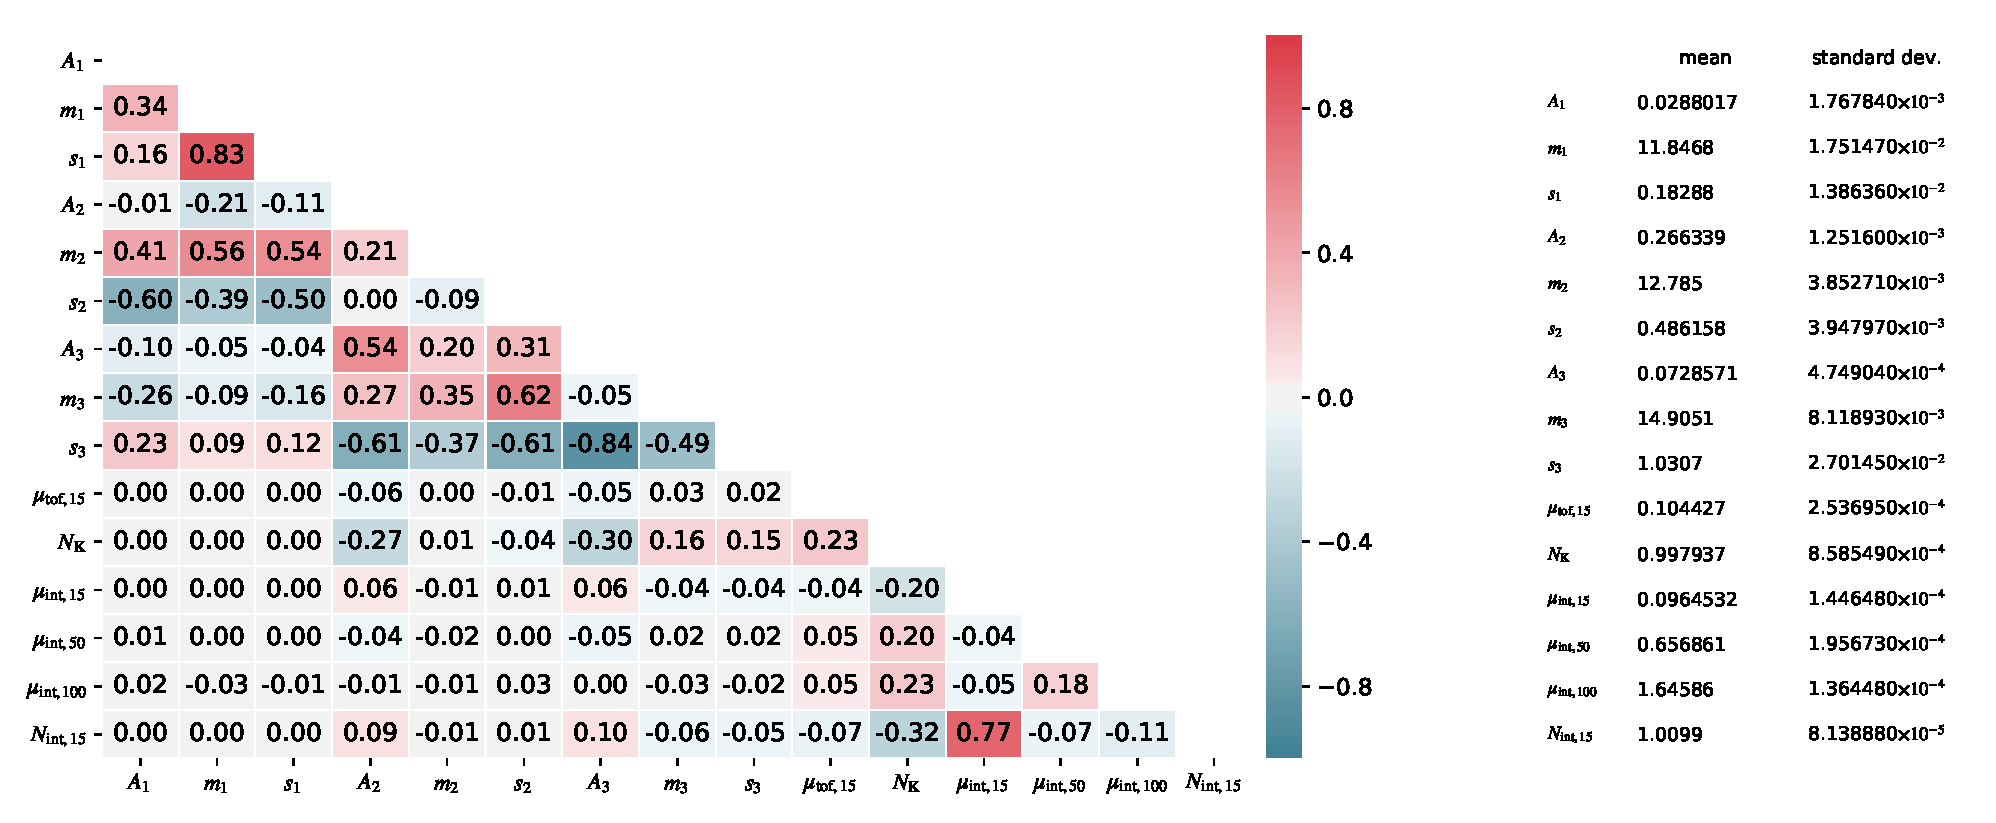
\includegraphics[width=\textwidth]{chapter/sensitivityStudyWithPreliminaryKatrinElossModel/appendix/fig/katrinElossParamValues.pdf}
    
    \glsaddall
    \printglossary[type=\acronymtype]
	
	\chapter*{Bibliography}
    \addcontentsline{toc}{chapter}{Bibliography}
    \addcontentsline{toc}{section}{References}
    \printbibliography[notkeyword={katrinEloss}, notkeyword={katrinSoftware}, title={References}, heading=subbibliography]
    
    \printbibliography[keyword={katrinEloss}, title={Preliminary},  heading=subbibliography]
    \addcontentsline{toc}{section}{Preliminary}
    
 	\printbibliography[keyword={katrinSoftware}, title={Software},  heading=subbibliography]
 	\addcontentsline{toc}{section}{Software}
 	
    %\chapter*{Acknowledgments}
I am convinced that there is always something new to learn. Nonetheless, handing in this work is the final act within my official education. It has been a long journey. 

I would like to express my gratitude to the people who helped me in completing this thesis:

First, I would like to thank Prof.~Dr.~Guido Drexlin for being the reviewer of this thesis and giving me the opportunity to work at the KATRIN experiment.

Special thanks goes to Dr.~Kathrin Valerius as the leader of the Young Investigator Group that I enjoyed being part of over the course of my thesis. Thank you for the warm welcome, that you made it possible for me to visit the MIT, and that you always made time, when I needed to discuss something. And, of course, thank you, for being the second reviewer of this thesis. 

I would also like to thank my adviser Moritz Machatschek. Thank you for your enthusiasm when tackling my physics problems as if they were your own. Also, thank you for frequently cross-checking my ideas, hinting me towards errors and offering solutions. Especially, thank you for your easygoing and calm attitude. It was a good experience having you as an adviser.

I would also like to thank Dr.~Valérian Sibille. Thank you for advising me before, during and after my stay at the MIT. And thank you for enabling my stay in the first place. I also really appreciate the great deal of time you took for reviewing my program code and teaching me software engineering as well as physics - and (maybe unintentionally) food culture.

I would also like to thank Dr.~Won-Qook Choi. Thank you for being such a cheerful and kind person. And thank you for frequently giving me the opportunity to express my opinion in software matters and appreciating my ideas. Also, thank you for helping me with analysis problems and for the many discussions.


I would also like to thank Dr.~Hendrik Seitz-Moskaliuk. Thank you for having been a pleasant office mate and for always promptly addressing my questions. Also, thank you for being the first to proofread pages of my thesis. Your feedback doubtlessly influenced my further writing style.

I would also like to thank Dr.~Jan Behrens. Thank you for proofreading a chapter of my thesis and for helping me many times with the computer infrastructure.


Also, I would like to thank the further proofreader Dr.~Volker Hannen, the rest of the Young Investigator Group and the people at KATRIN that helped me on a daily basis - be it practically or motivational: Thomas Csabo, Klaus Mehret, Joachim Wolf, Lutz Schimpf, Dr.~Stephanie Hickford, Dr.~Carsten Röttele, Dr.~Florian Heizmann, Rudolf Sack, Fabian Block, Leonard Köllenberger, Ferenc Glück and the ones I forgot. 


In a broader scope, I would like to thank my friends and family for always supporting me during my education. Especially, I want to mention my parents and my sisters. Thank you.
\end{document}
